%yright 2007, 2008, 2009 Elsevier Ltd
%% 
%% This file is part of the 'Elsarticle Bundle'.
%% ---------------------------------------------
%% 
%% It may be distributed under the conditions of the LaTeX Project Public
%% License, either version 1.2 of this license or (at your option) any
%% later version.  The latest version of this license is in
%%    http://www.latex-project.org/lppl.txt
%% and version 1.2 or later is part of all distributions of LaTeX
%% version 1999/12/01 or later.
%% 
%% The list of all files belonging to the 'Elsarticle Bundle' is
%% given in the file `manifest.txt'.
%% 

%% Template article for Elsevier's document class `elsarticle'
%% with numbered style bibliographic references
%% SP 2008/03/01

% \documentclass[preprint,11pt]{elsarticle}
\section{Soft drop method in future collider performance}
In this section, we use the specific method about the soft-drop to study the performance of the detector in the different cell sizes.  In the Figure , , , , are the distribution of the signal and background. 
\subsection{Analysis method}
In this analysis, We fix the central at the median in signal distribution, and we use the different width to open the window to draw ROC curves.
\subsection{The conclusion of the results}

 
%50bins
\begin{figure}
\begin{center}
   \subfigure[5TeV at 20$\times$20(cm$\times$cm) in cluster] {
   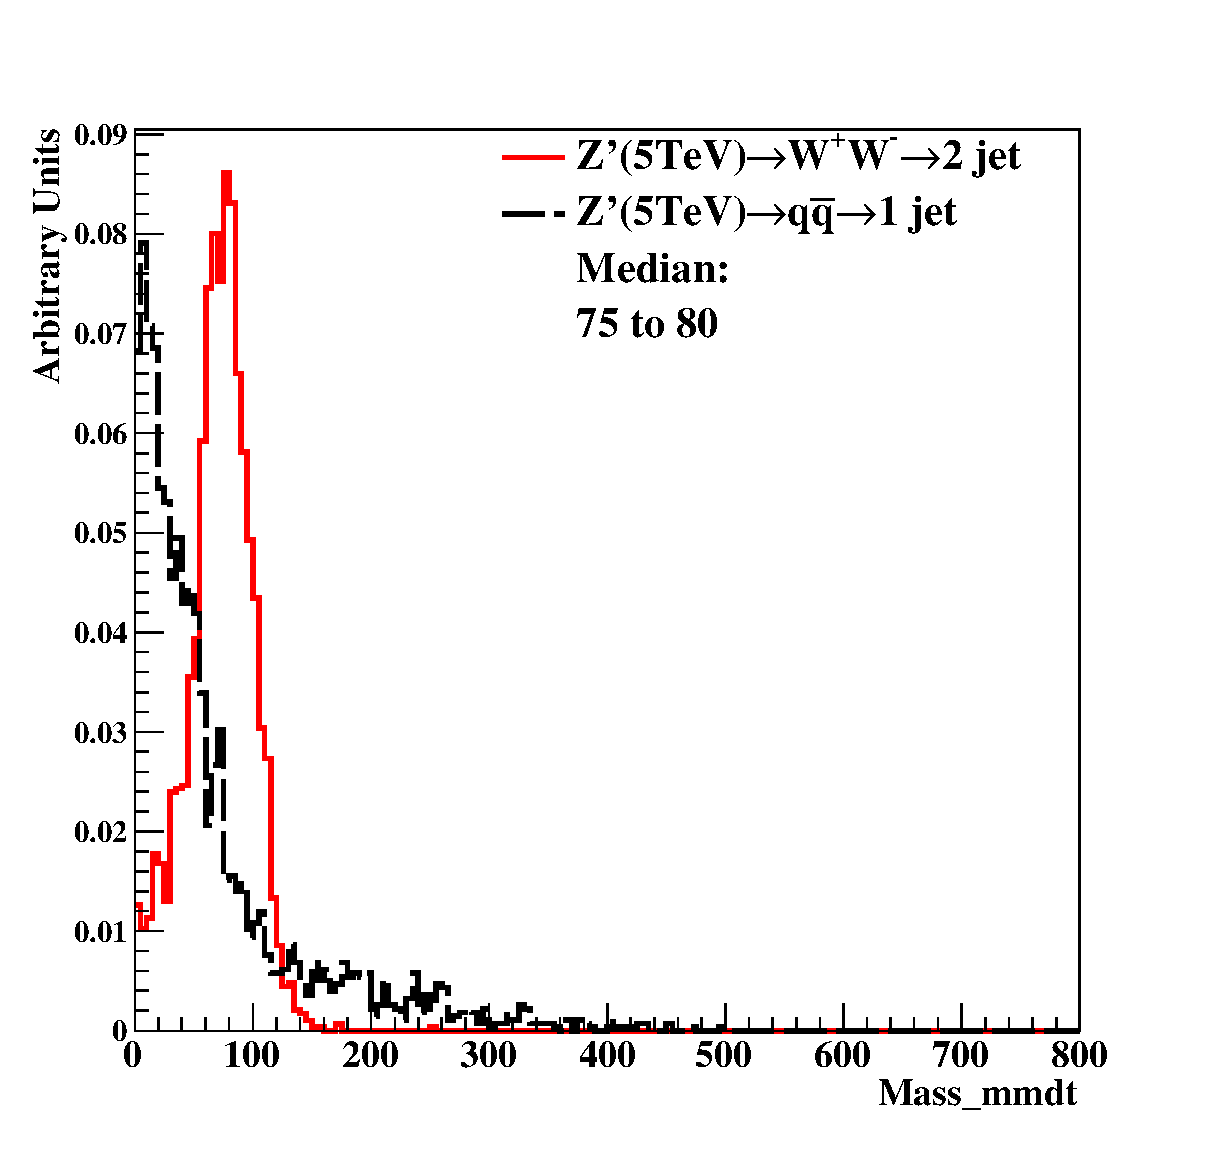
\includegraphics[width=0.22\textwidth]{figs/Dis_cluster_010_mass_mmdt_5tev_04.eps}
   }
      \subfigure[10TeV at 20$\times$20(cm$\times$cm) in cluster] {
   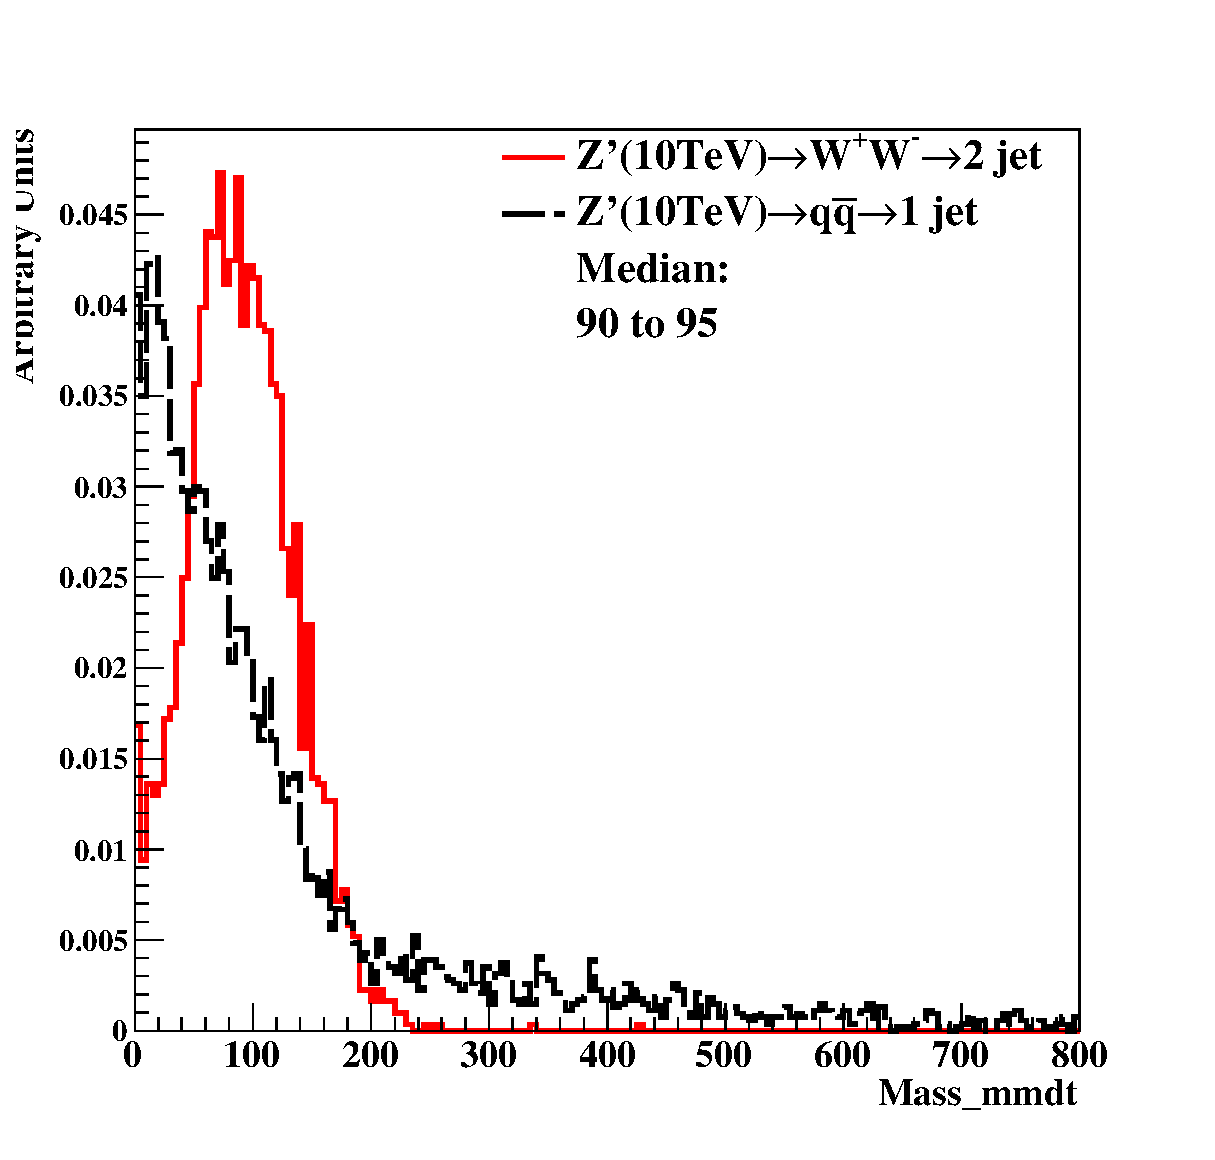
\includegraphics[width=0.22\textwidth]{figs/Dis_cluster_010_mass_mmdt_10tev_04.eps}
   }
   \subfigure[20TeV at 20$\times$20(cm$\times$cm) in cluster] {
   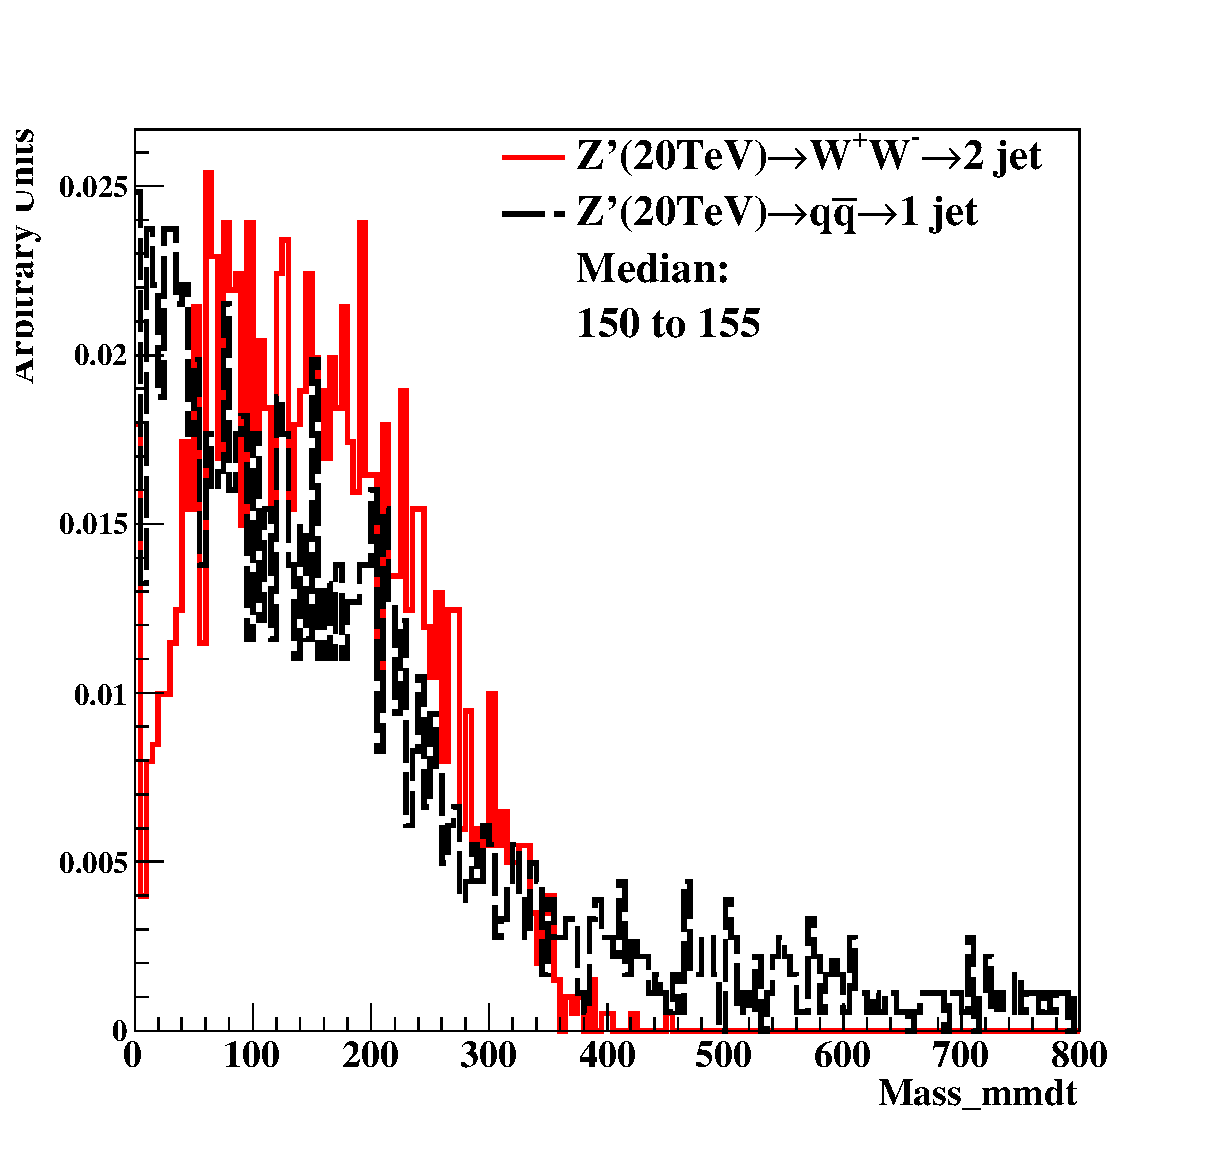
\includegraphics[width=0.22\textwidth]{figs/Dis_cluster_010_mass_mmdt_20tev_04.eps}
   }
    \subfigure[40TeV at 20$\times$20(cm$\times$cm) in cluster] {
   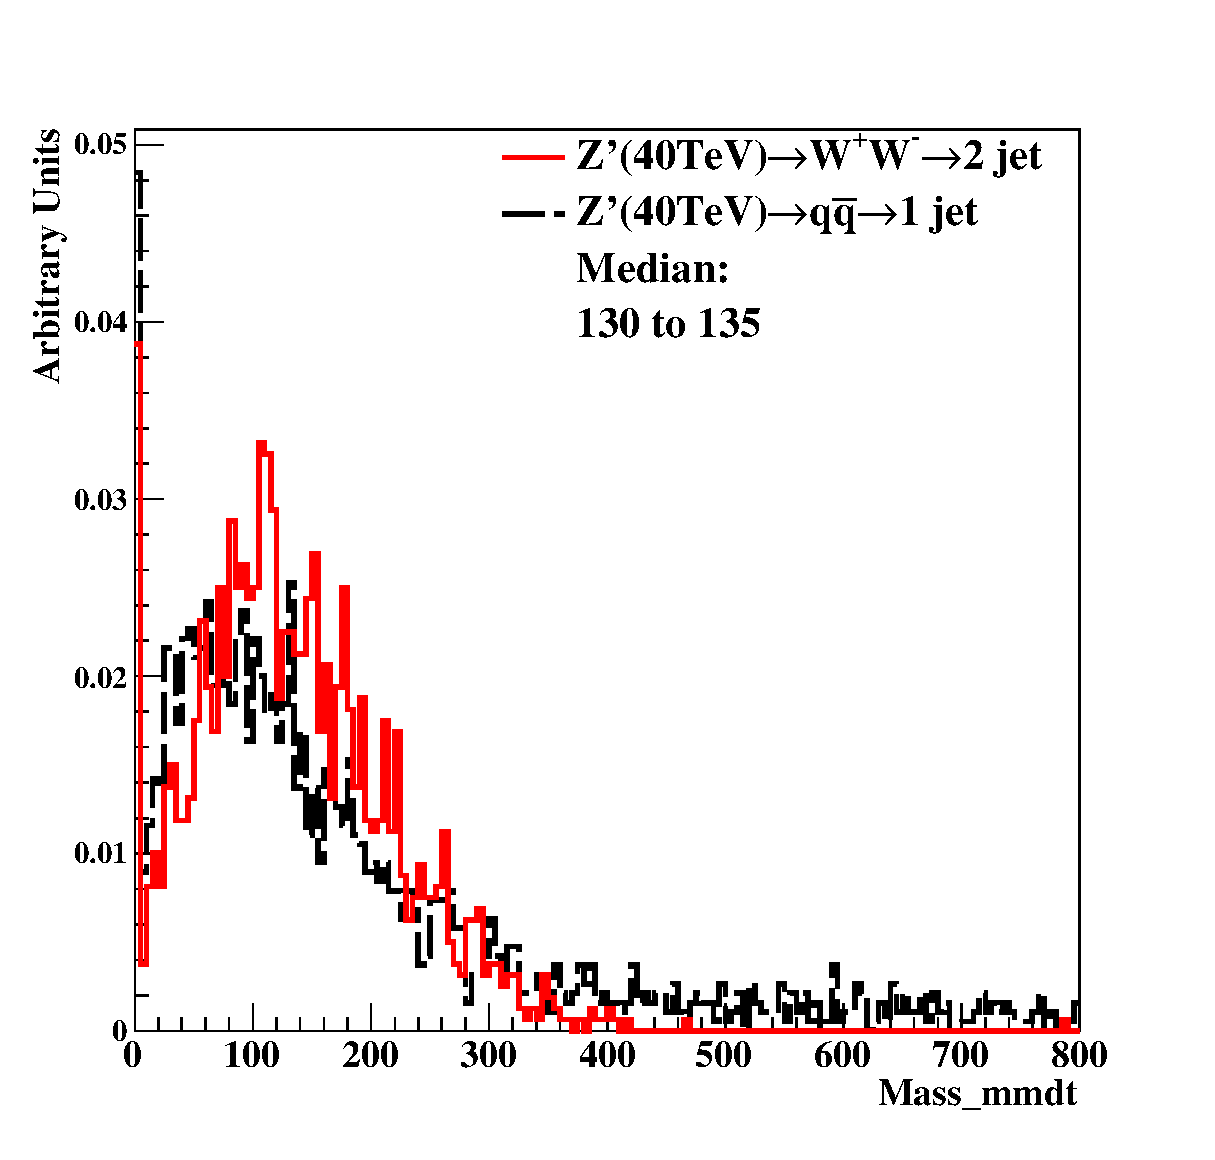
\includegraphics[width=0.22\textwidth]{figs/Dis_cluster_010_mass_mmdt_40tev_04.eps}
   }
   \subfigure[5TeV at 5$\times$5(cm$\times$cm) in cluster] {
   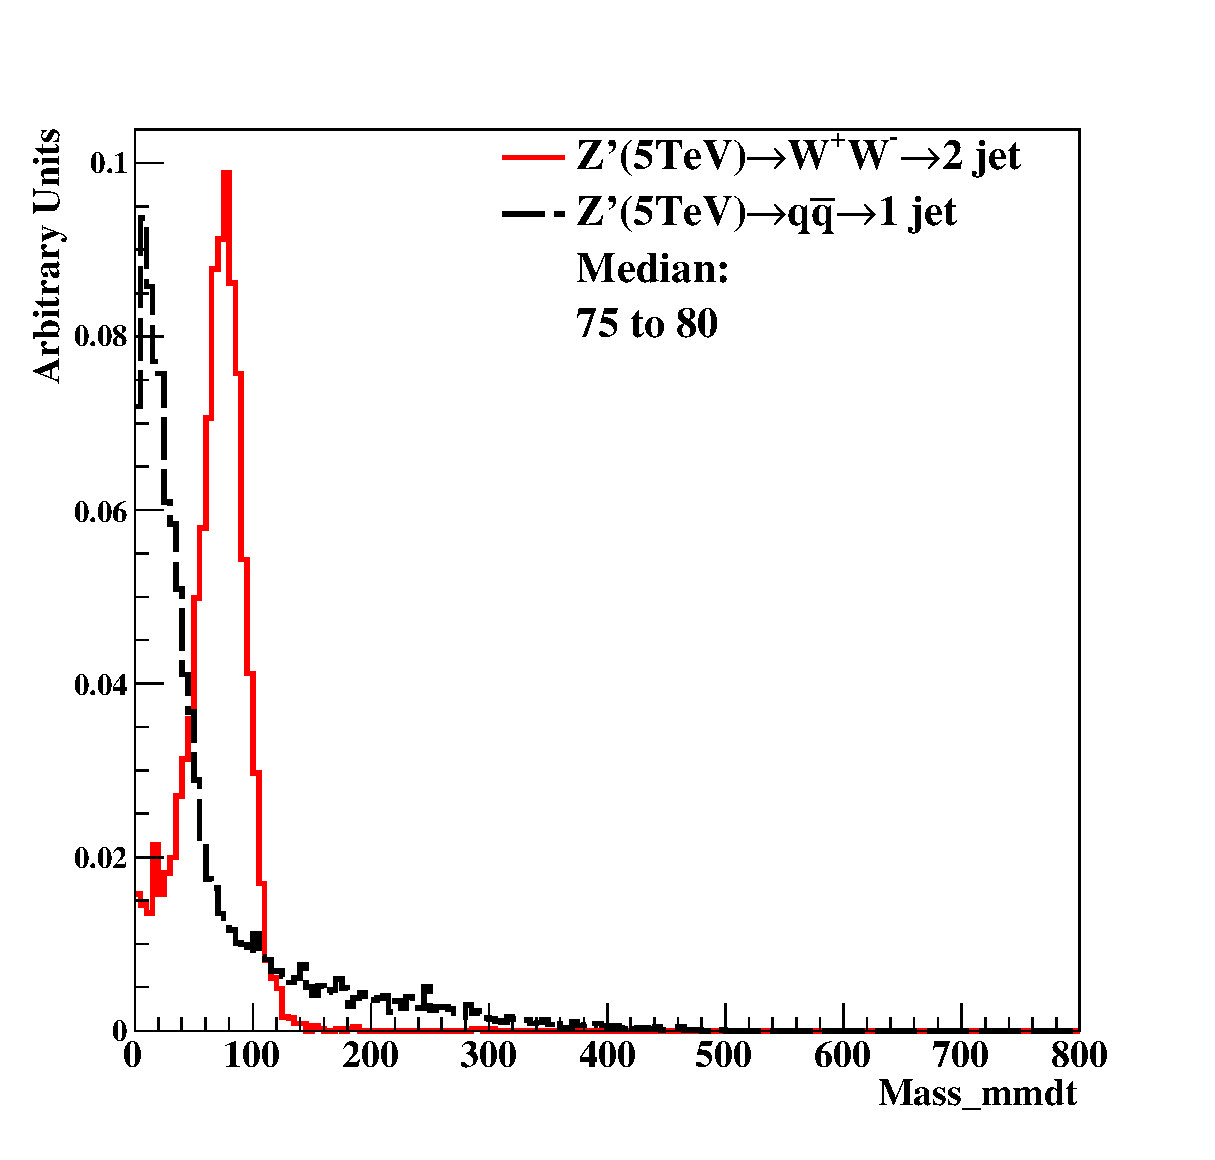
\includegraphics[width=0.22\textwidth]{figs/Dis_cluster_009_mass_mmdt_5tev_04.eps}
   }
   \subfigure[10TeV at 5$\times$5(cm$\times$cm) in cluster] {
   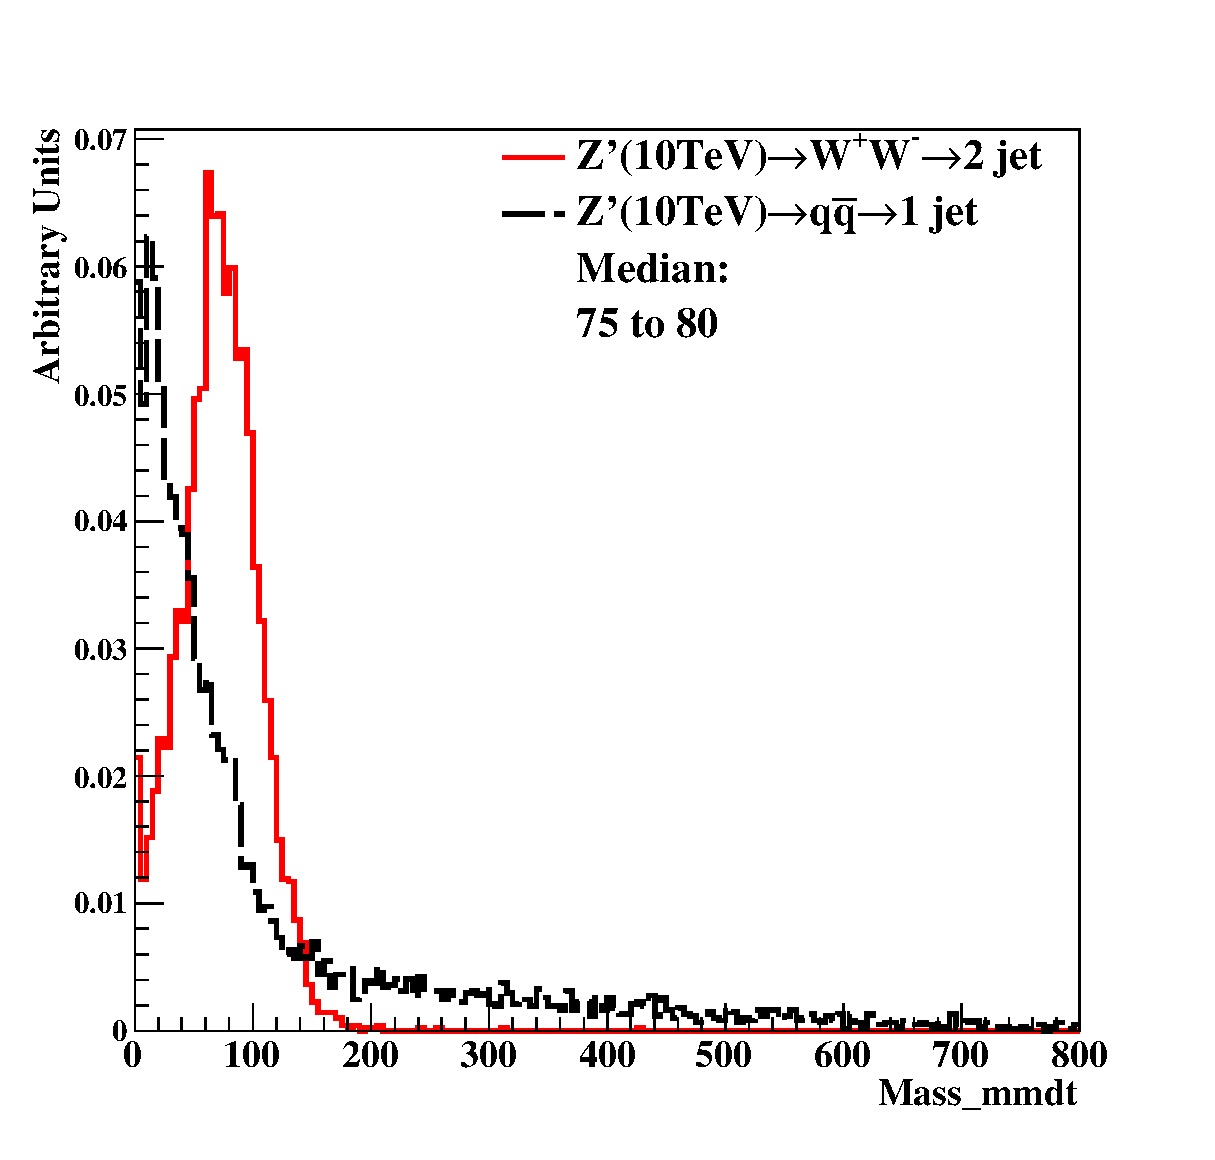
\includegraphics[width=0.22\textwidth]{figs/Dis_cluster_009_mass_mmdt_10tev_04.eps}
   }
      \subfigure[20TeV at 5$\times$5(cm$\times$cm) in cluster] {
   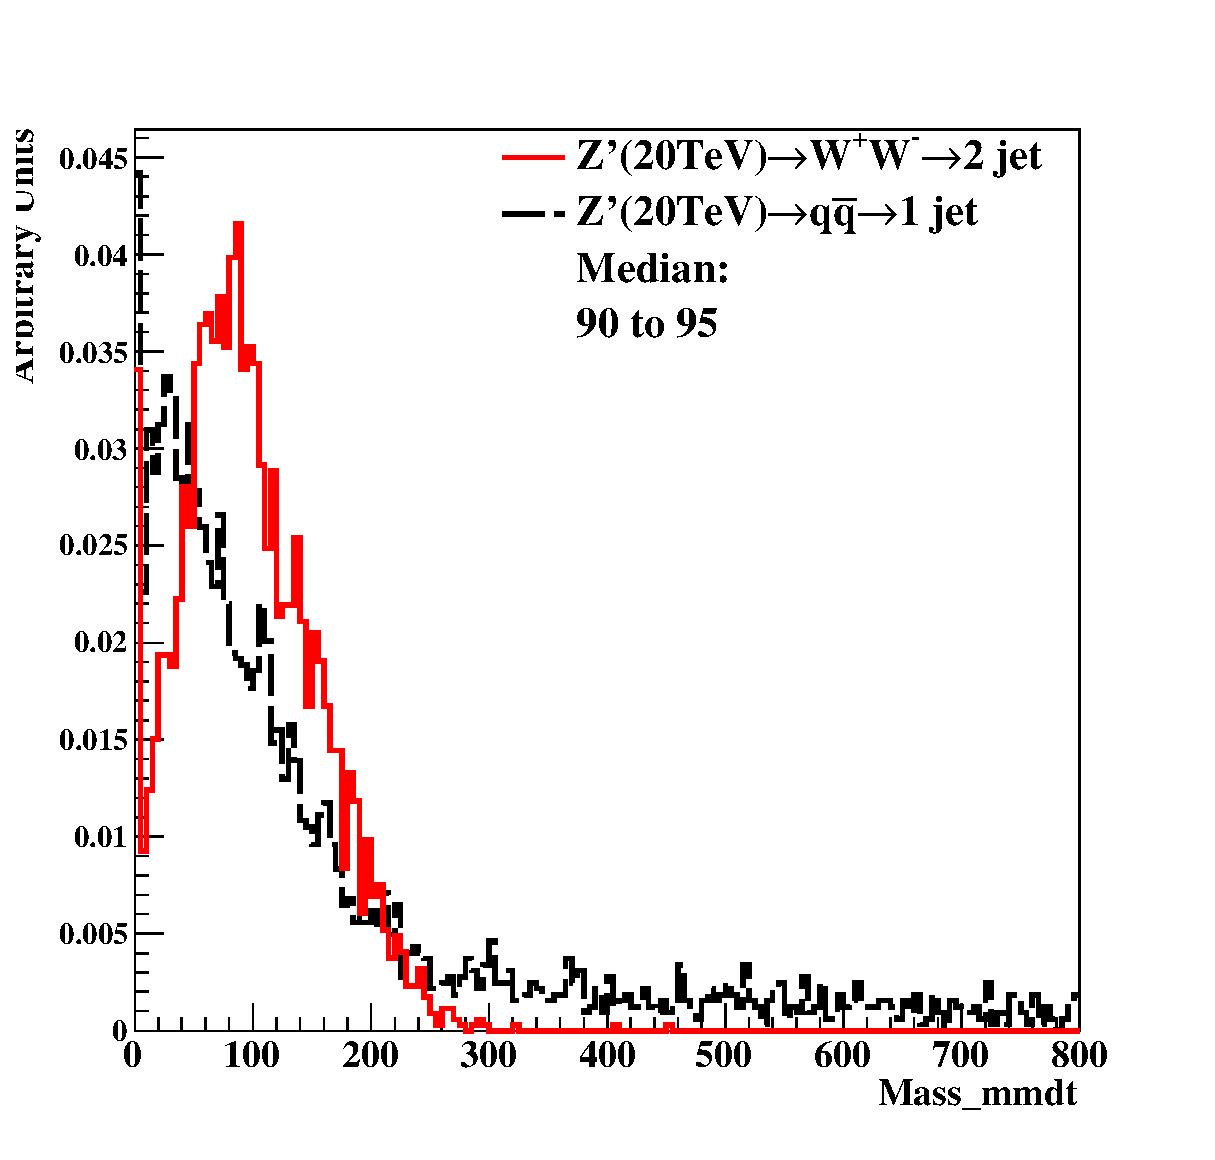
\includegraphics[width=0.22\textwidth]{figs/Dis_cluster_009_mass_mmdt_20tev_04.eps}\hfill
   }
      \subfigure[40TeV at 5$\times$5(cm$\times$cm) in cluster] {
   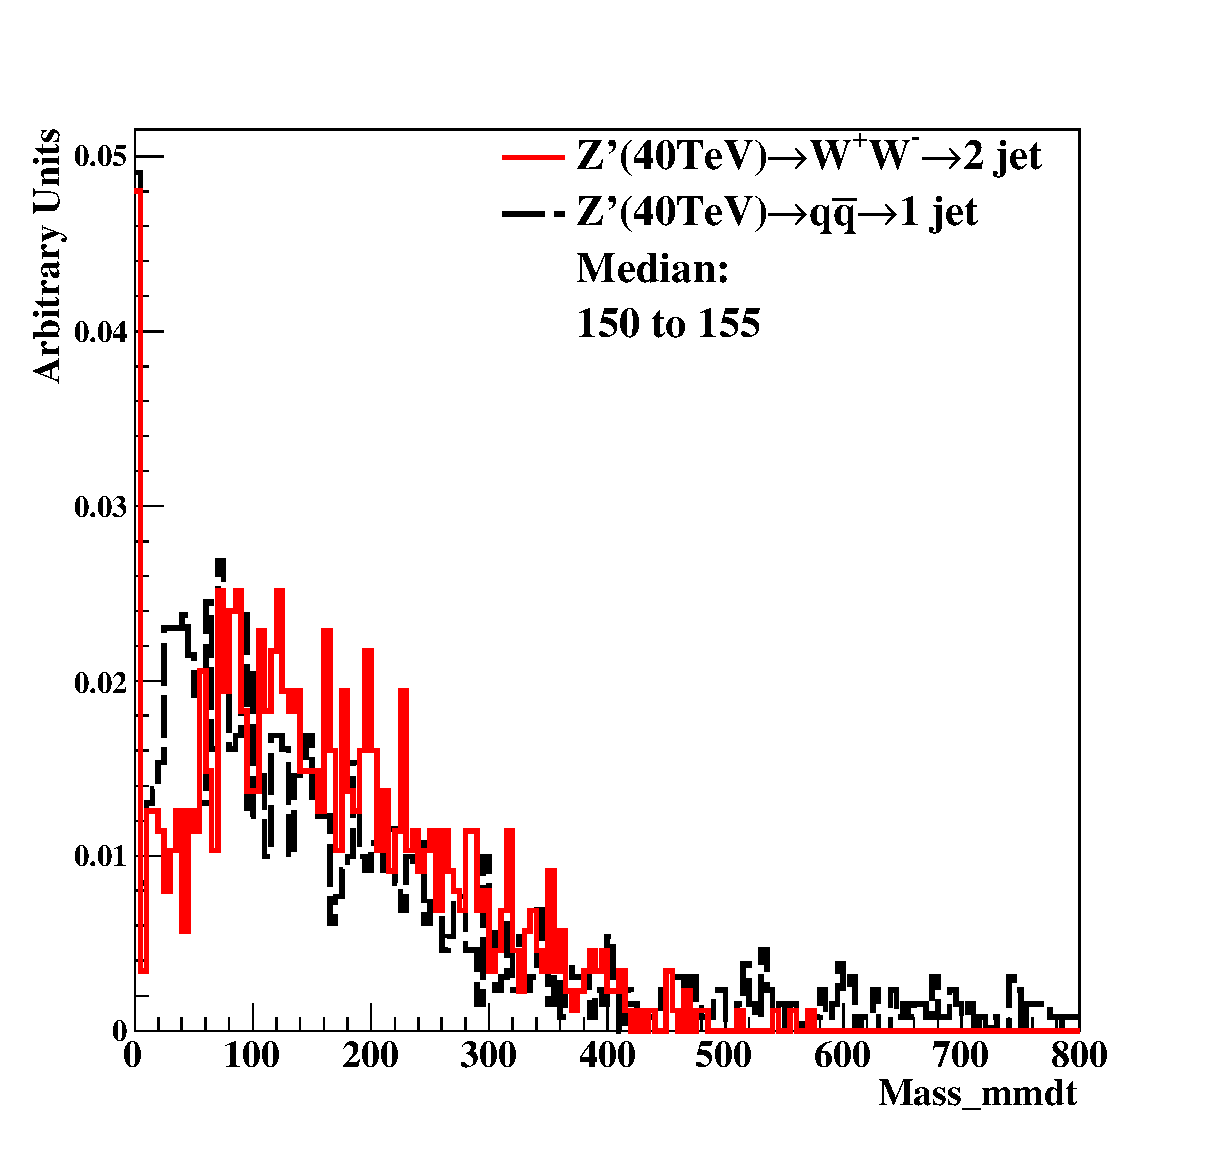
\includegraphics[width=0.22\textwidth]{figs/Dis_cluster_009_mass_mmdt_40tev_04.eps}\hfill
   }
   \subfigure[5TeV at 1$\times$1(cm$\times$cm) in cluster] {
   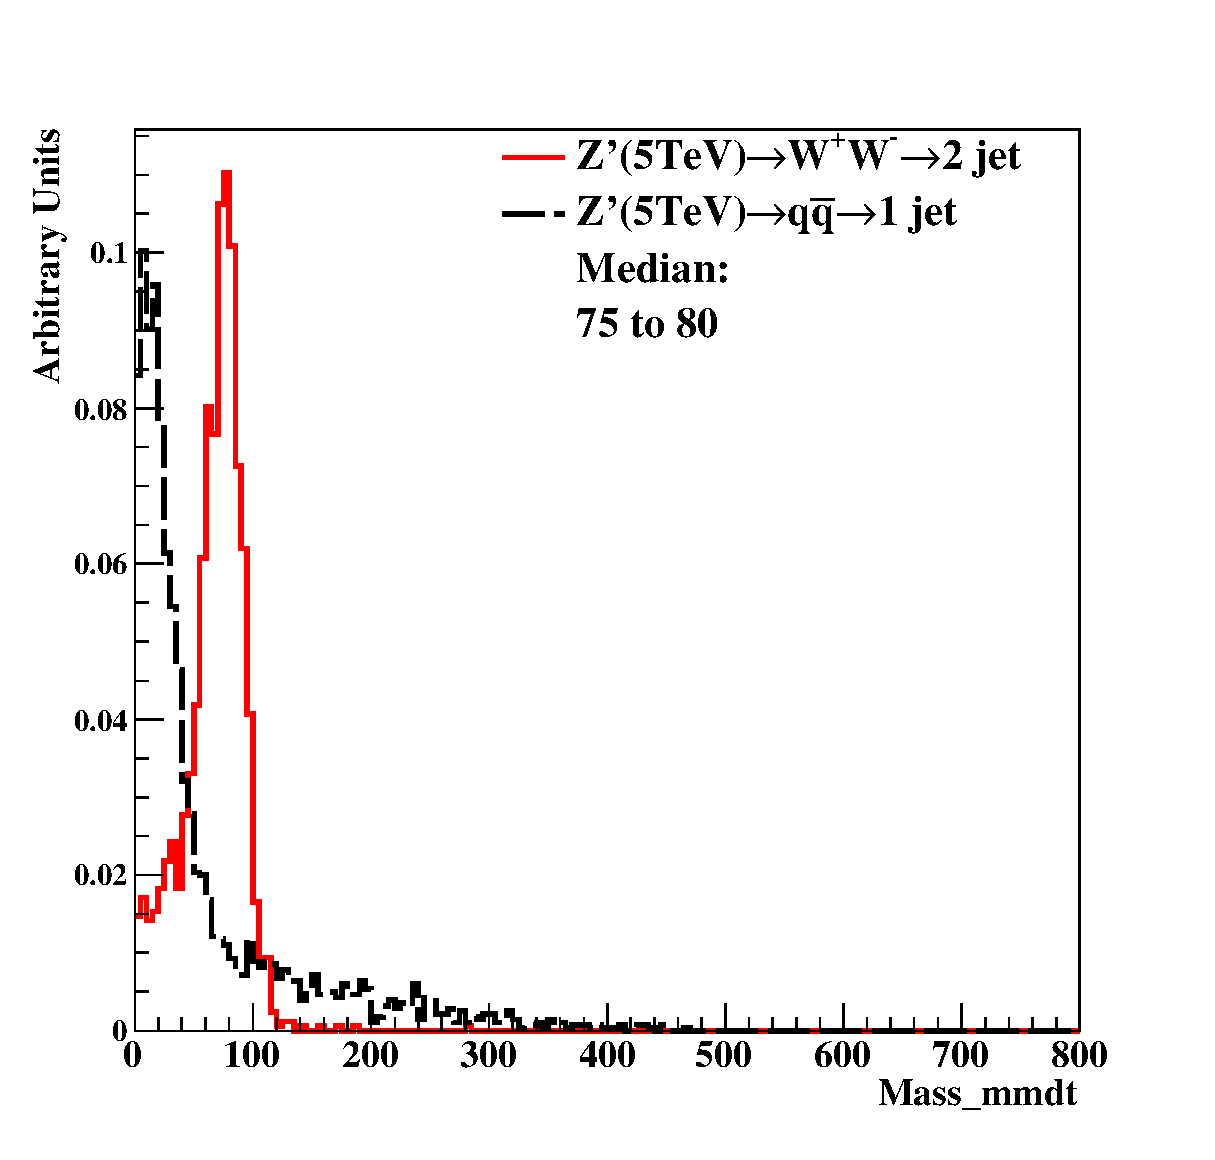
\includegraphics[width=0.22\textwidth]{figs/Dis_cluster_012_mass_mmdt_5tev_04.eps}\hfill
   }
    \subfigure[10TeV at 1$\times$1(cm$\times$cm) in cluster] {
   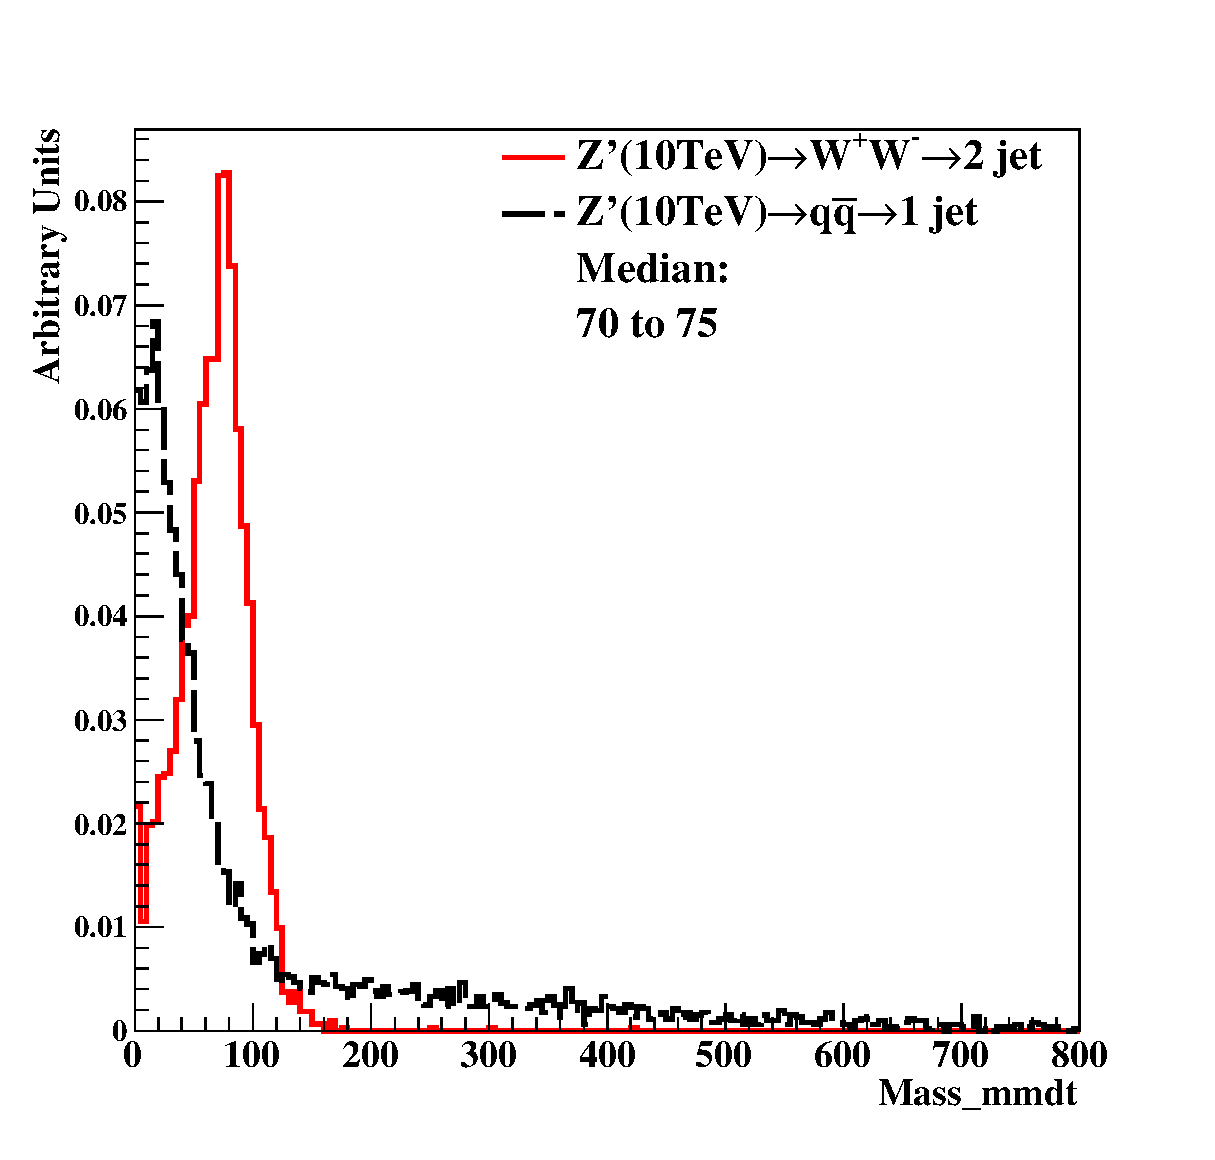
\includegraphics[width=0.22\textwidth]{figs/Dis_cluster_012_mass_mmdt_10tev_04.eps}
   }
   \subfigure[20TeV at 1$\times$1(cm$\times$cm) in cluster] {
   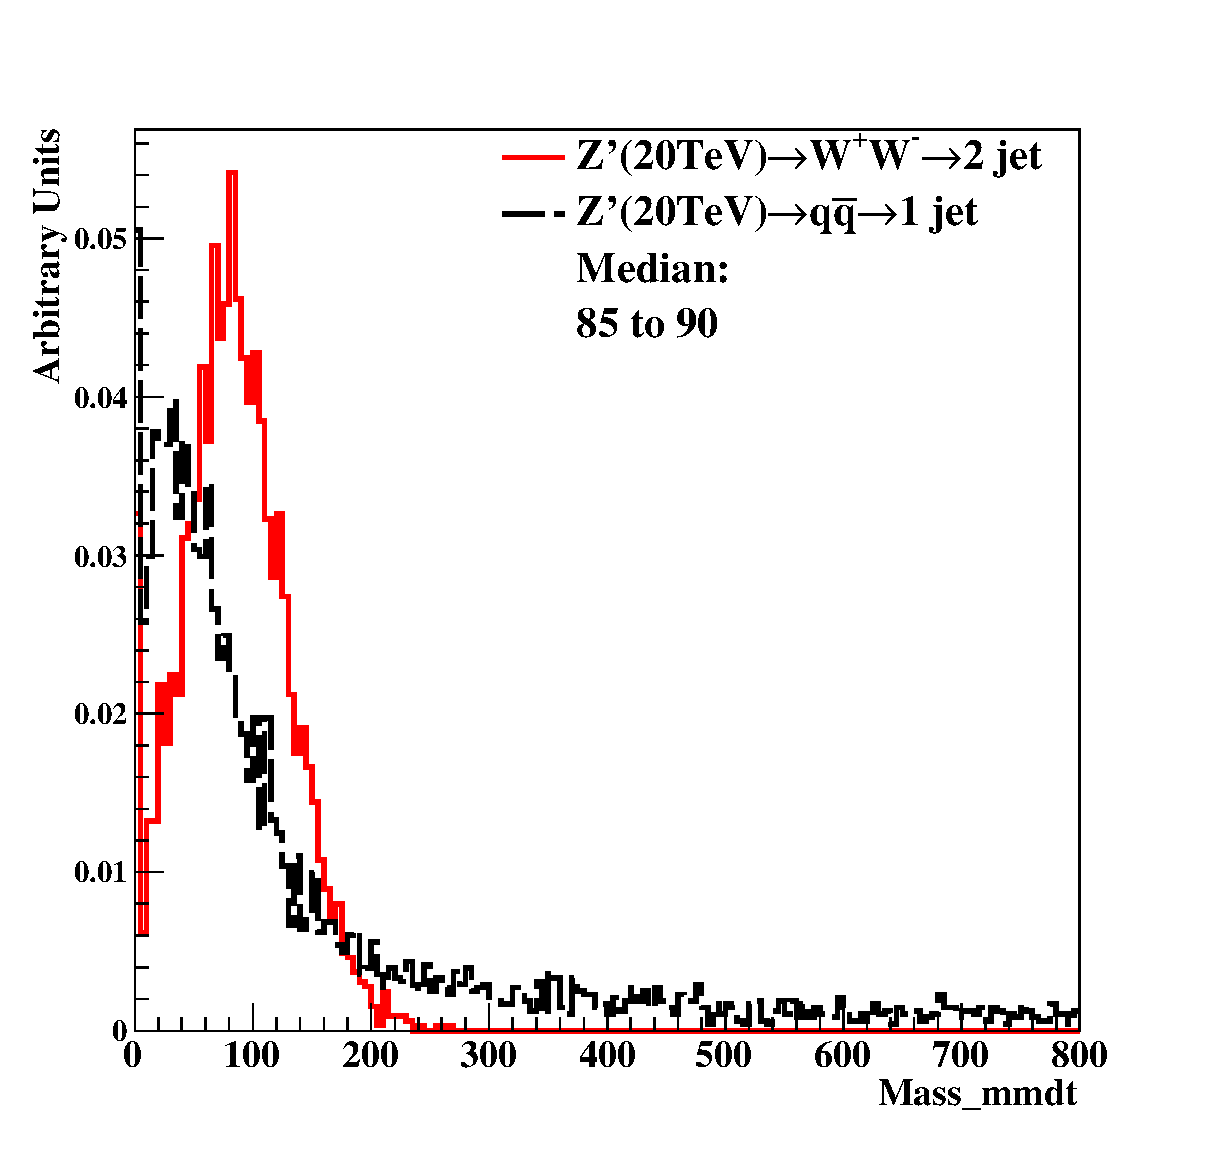
\includegraphics[width=0.22\textwidth]{figs/Dis_cluster_012_mass_mmdt_20tev_04.eps}\hfill
   }
      \subfigure[40TeV at 1$\times$1(cm$\times$cm) in cluster] {
   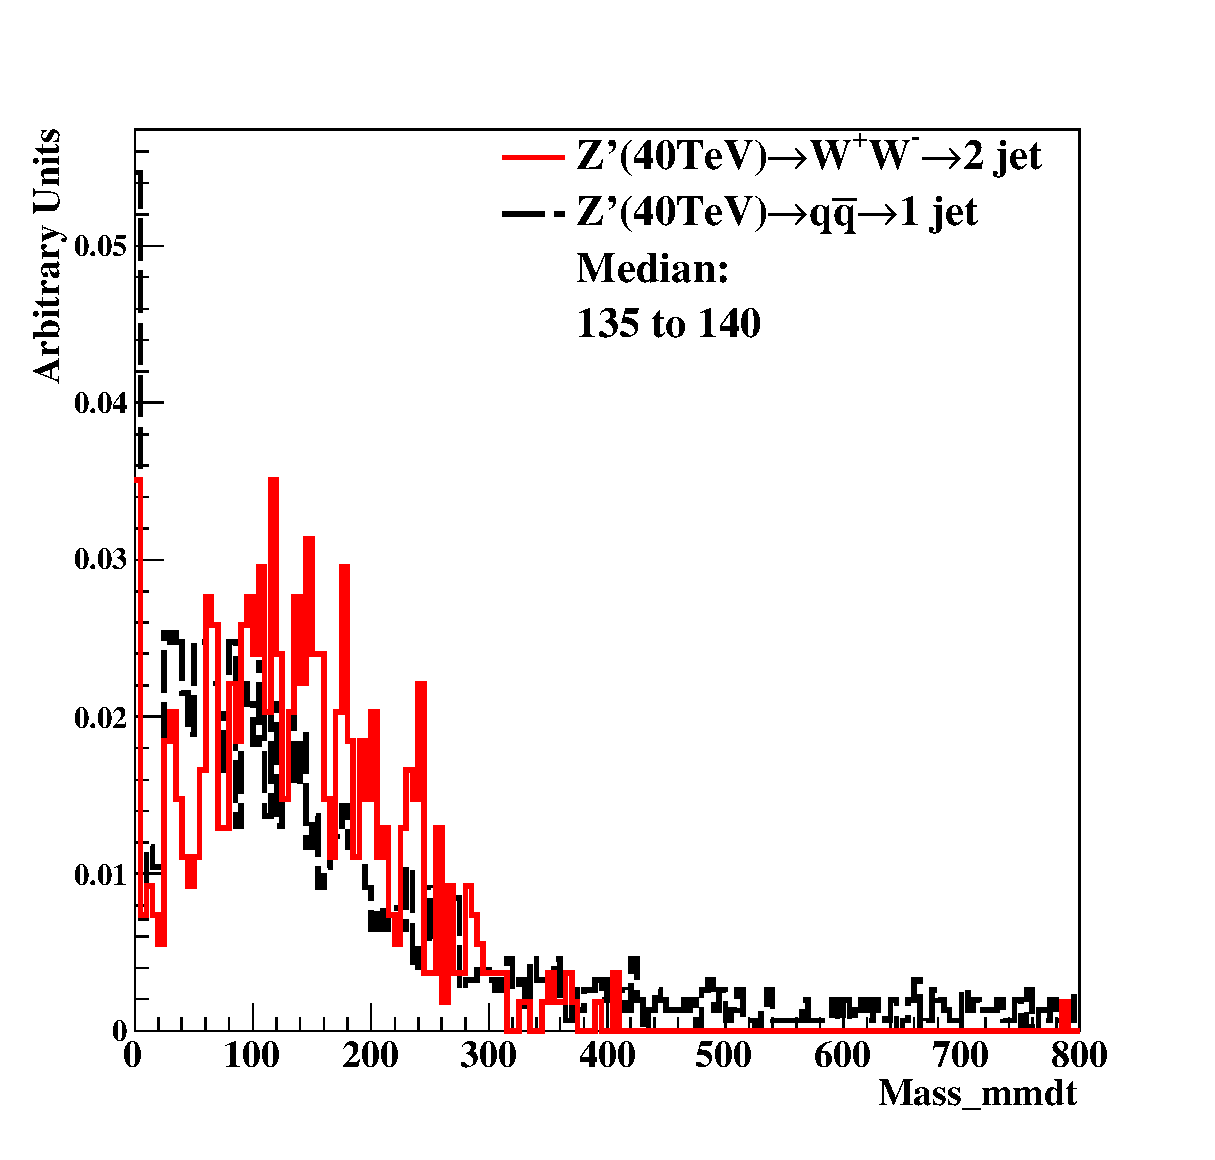
\includegraphics[width=0.22\textwidth]{figs/Dis_cluster_012_mass_mmdt_40tev_04.eps}
   }

\end{center}
\caption{Distributions of mass soft drop at $\beta$=0, signal=ww, in 5,10TeV energy of collision  in different detector sizes. Cell Size in 20$\times$20, 5$\times$5, and 1$\times$1(cm$\times$cm) are shown here.}
\label{fig:cluster_tau21_tau32}
\end{figure}

\begin{figure}
\begin{center}
  \subfigure[Central at Median($20\times20$=80,$5\times5$=80,$1\times1$=80) change width in cluster at 5TeV] {
  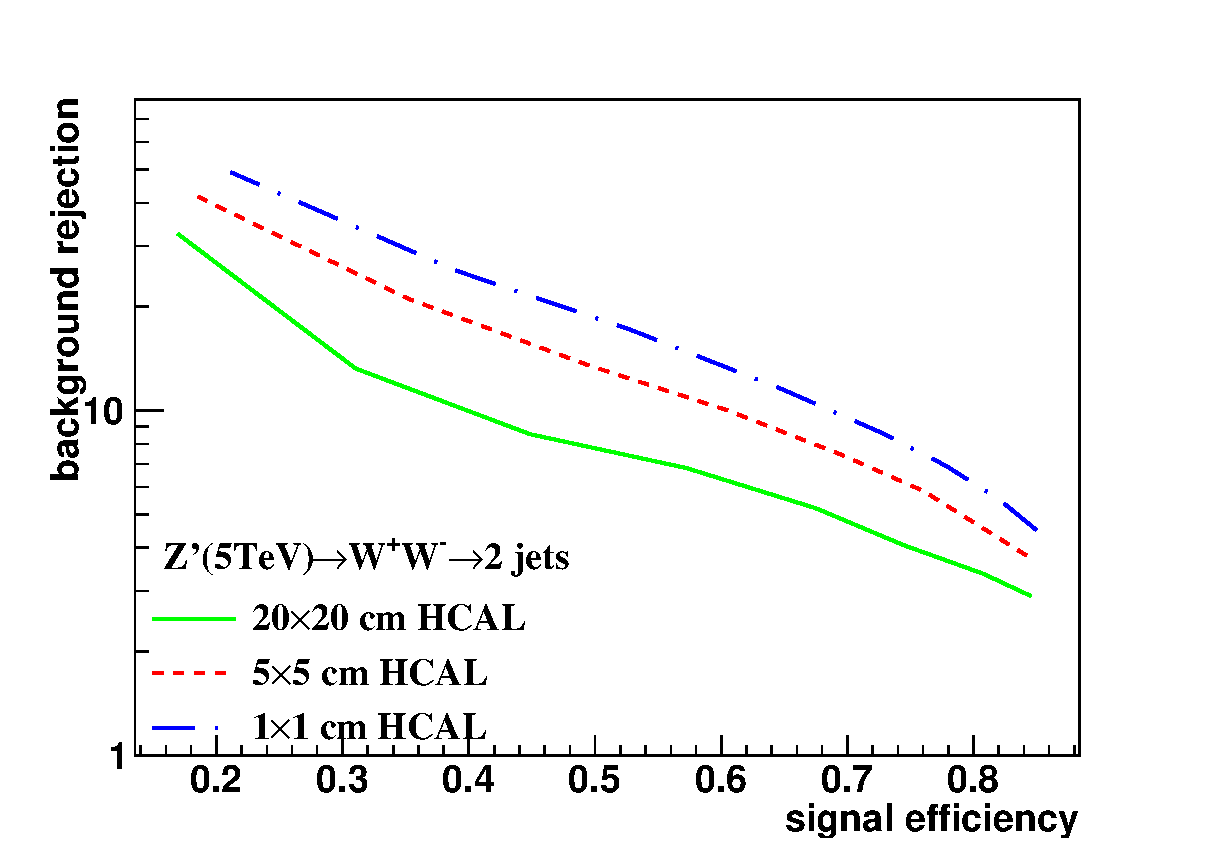
\includegraphics[width=0.43\textwidth]{figs/A_Cluster_mass_mmdt_5tev_eff_1_central_fix_ww_qq_log.eps}
  }
  \subfigure[Central at Median($20\times20$=95,$5\times5$=80,$1\times1$=75) change width in cluster at 10TeV] {
  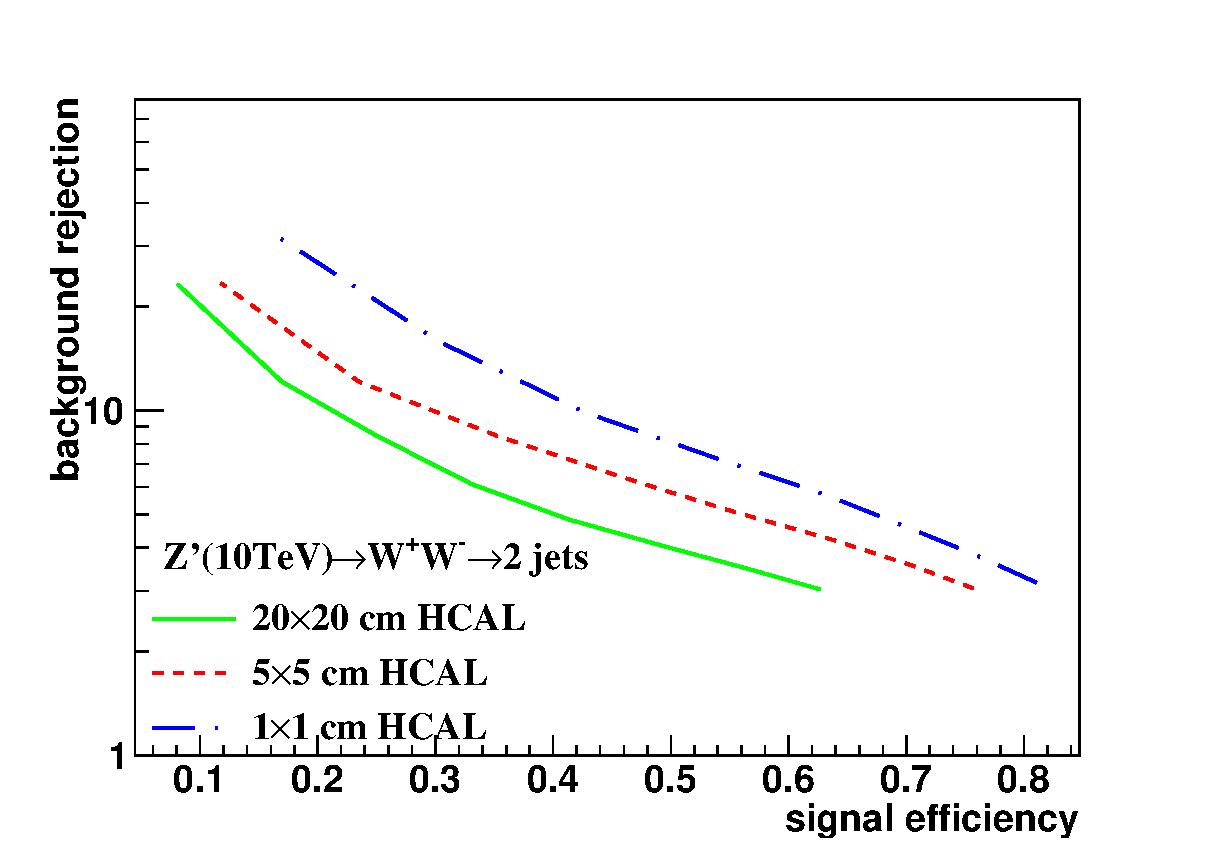
\includegraphics[width=0.43\textwidth]{figs/A_Cluster_mass_mmdt_10tev_eff_1_central_fix_ww_qq_log.eps}
  }
 \subfigure[Central at Median($20\times20$=155,$5\times5$=95,$1\times1$=90) change width in cluster at 20TeV] {
 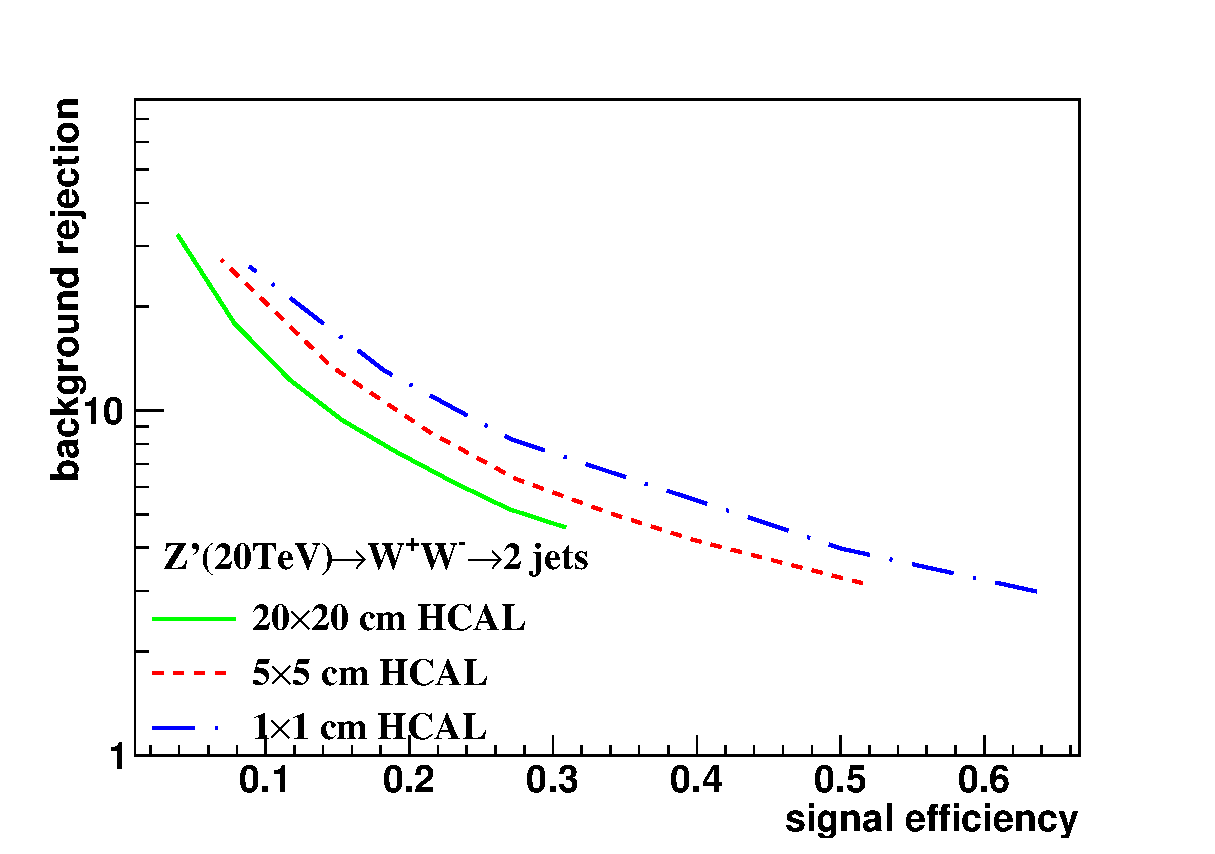
\includegraphics[width=0.43\textwidth]{figs/A_Cluster_mass_mmdt_20tev_eff_1_central_fix_ww_qq_log.eps}
 }
 \subfigure[Central at Median($20\times20$=130,$5\times5$=150,$1\times1$=135) change width in cluster at 40TeV] {
 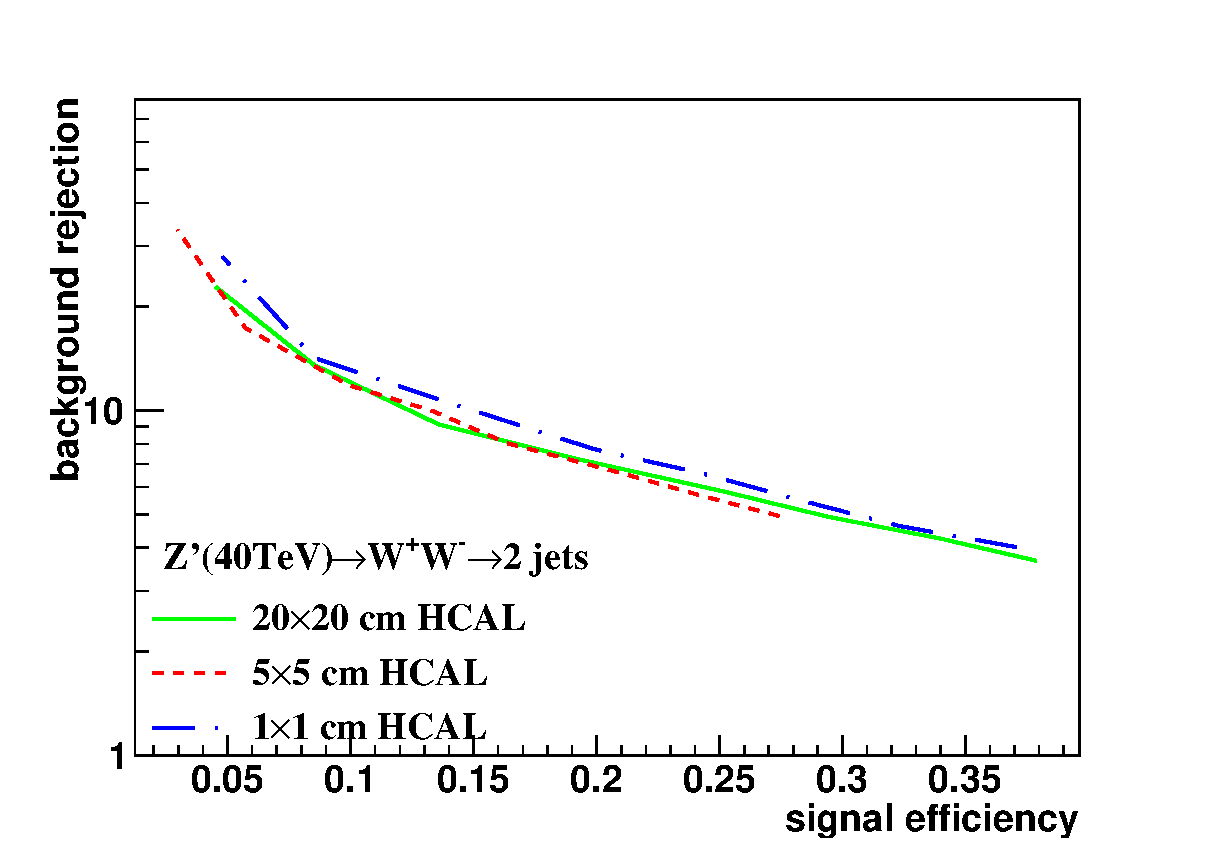
\includegraphics[width=0.43\textwidth]{figs/A_Cluster_mass_mmdt_40tev_eff_1_central_fix_ww_qq_log.eps}
 }
\end{center}
\caption{study of "fix central and change width" in mass soft drop at $\beta$=0, signal=ww, in 5, 10, 20, 40TeV energy of collision  in different detector sizes. Cell Size in 20$\times$20, 5$\times$5, and 1$\times$1(cm$\times$cm) are shown in each picture.}
\label{fig:cluster_tau21_tau32}
\end{figure}

\begin{figure}
\begin{center}
   \subfigure[5TeV at 20$\times$20(cm$\times$cm) in cluster] {
   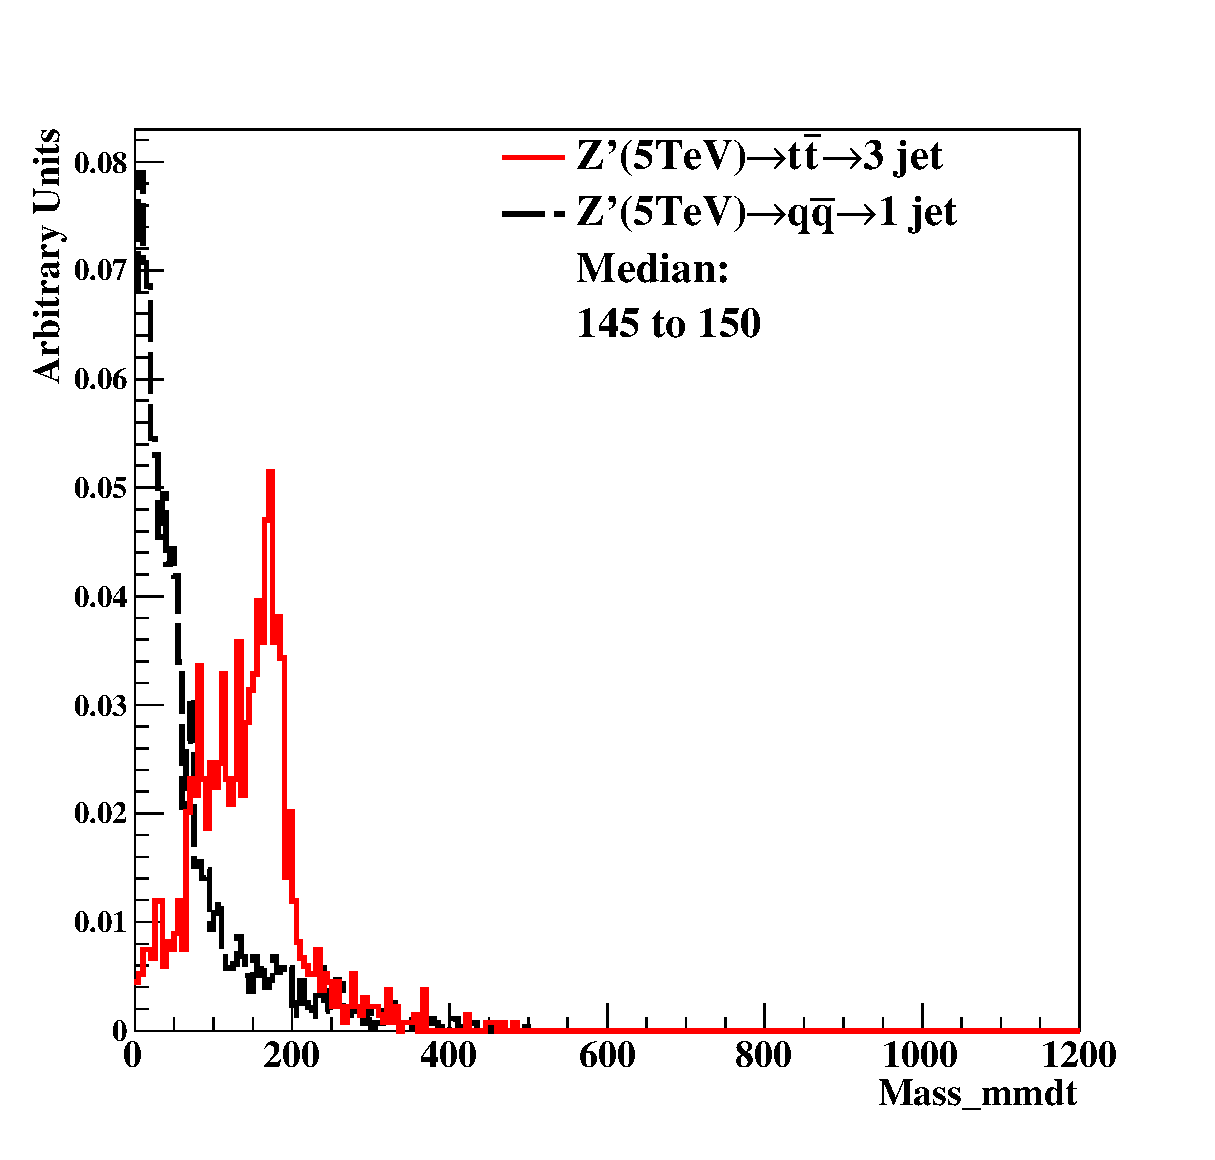
\includegraphics[width=0.22\textwidth]{figs/Dis_cluster_010_mass_mmdt_tt_5tev_04_tt.eps}
   }
      \subfigure[10TeV at 20$\times$20(cm$\times$cm) in cluster] {
   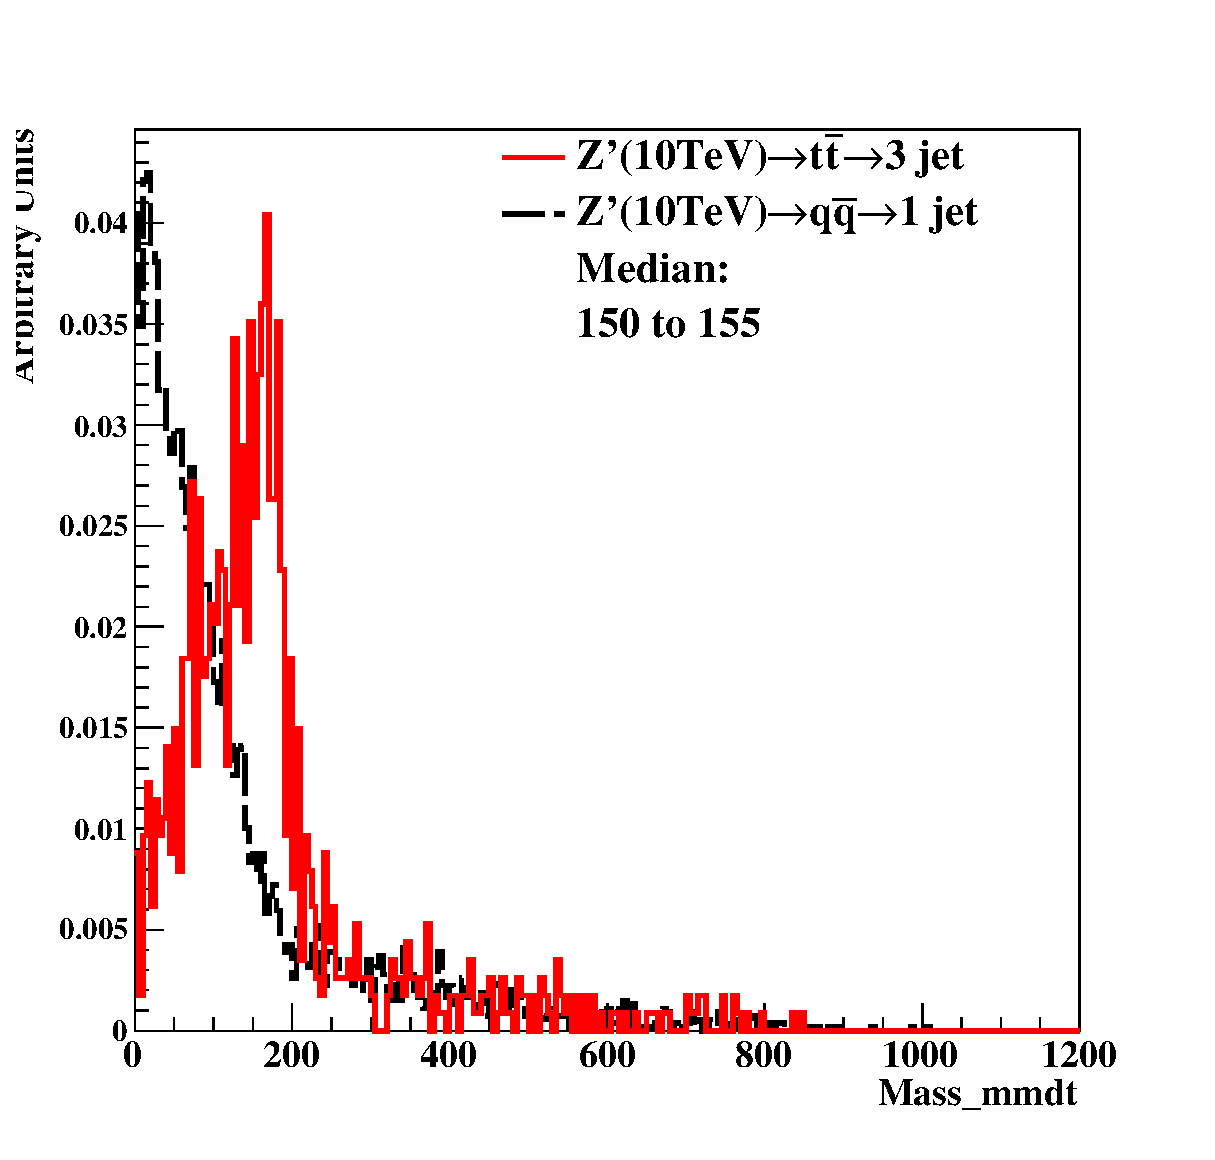
\includegraphics[width=0.22\textwidth]{figs/Dis_cluster_010_mass_mmdt_tt_10tev_04_tt.eps}
   }
   \subfigure[20TeV at 5$\times$5(cm$\times$cm) in cluster] {
   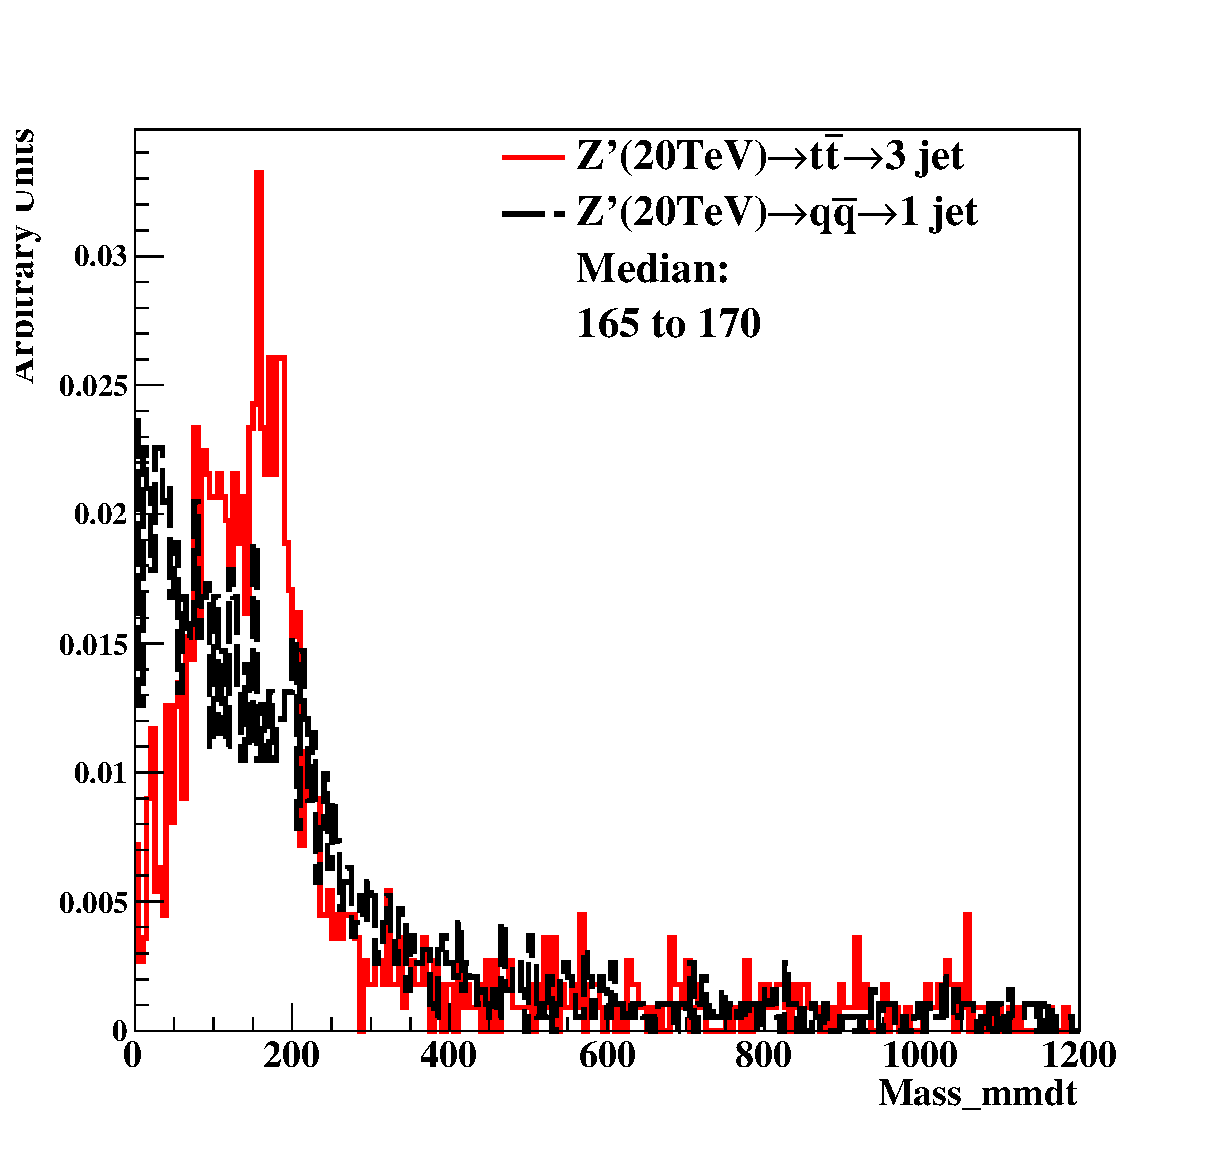
\includegraphics[width=0.22\textwidth]{figs/Dis_cluster_010_mass_mmdt_tt_20tev_04_tt.eps}
   }
    \subfigure[40TeV at 5$\times$5(cm$\times$cm) in cluster] {
   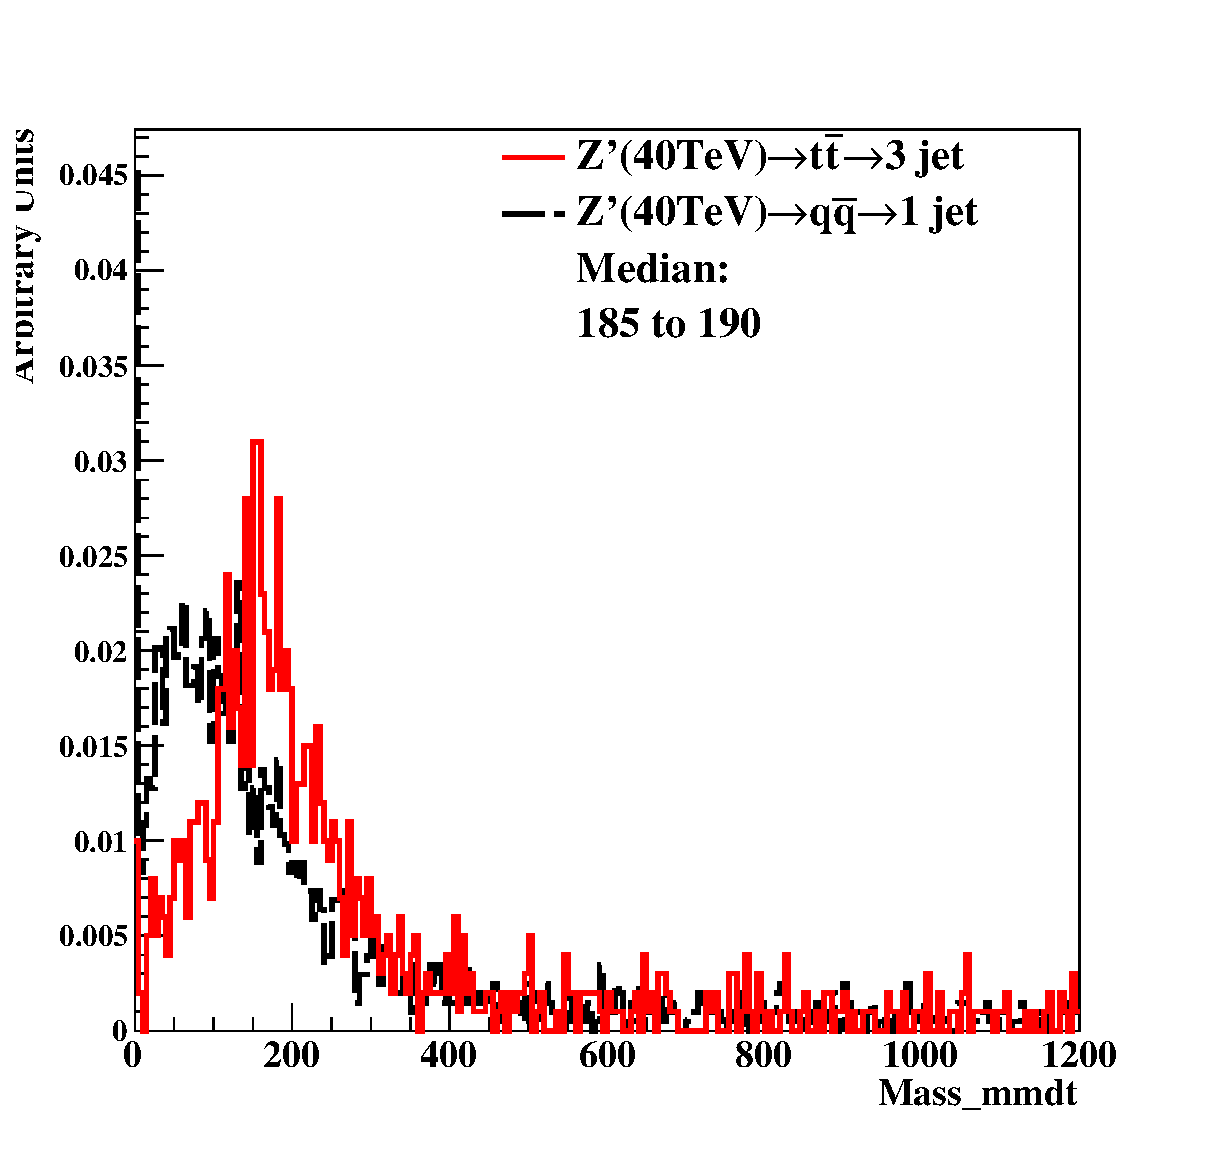
\includegraphics[width=0.22\textwidth]{figs/Dis_cluster_010_mass_mmdt_tt_40tev_04_tt.eps}
   }
   \subfigure[5TeV at 1$\times$1(cm$\times$cm) in cluster] {
   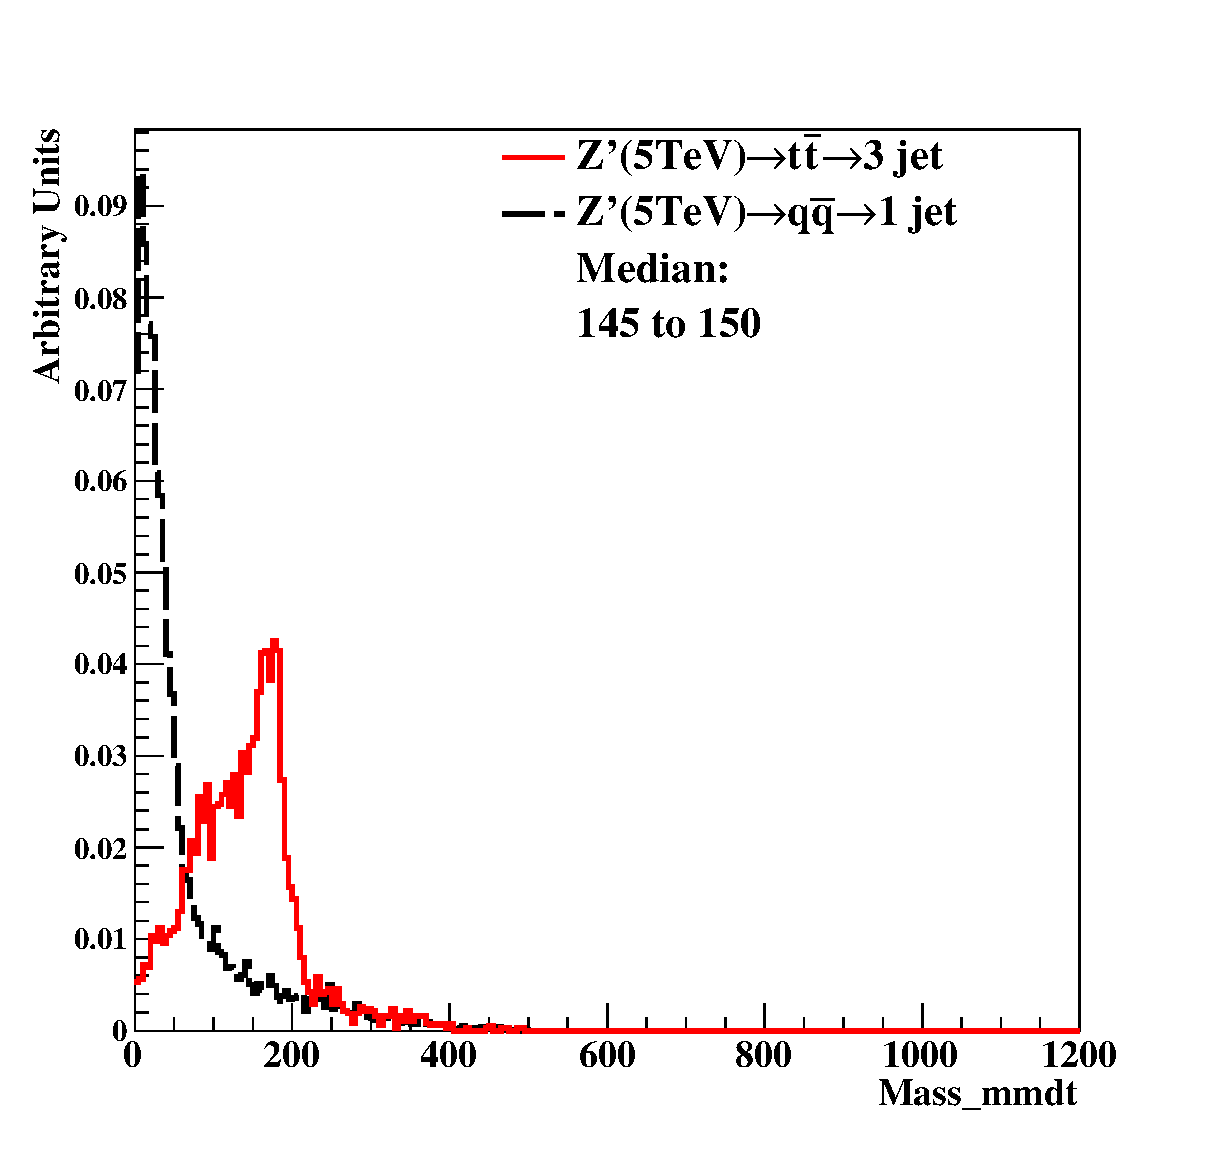
\includegraphics[width=0.22\textwidth]{figs/Dis_cluster_009_mass_mmdt_tt_5tev_04_tt.eps}
   }
   \subfigure[10TeV at 1$\times$1(cm$\times$cm) in cluster] {
   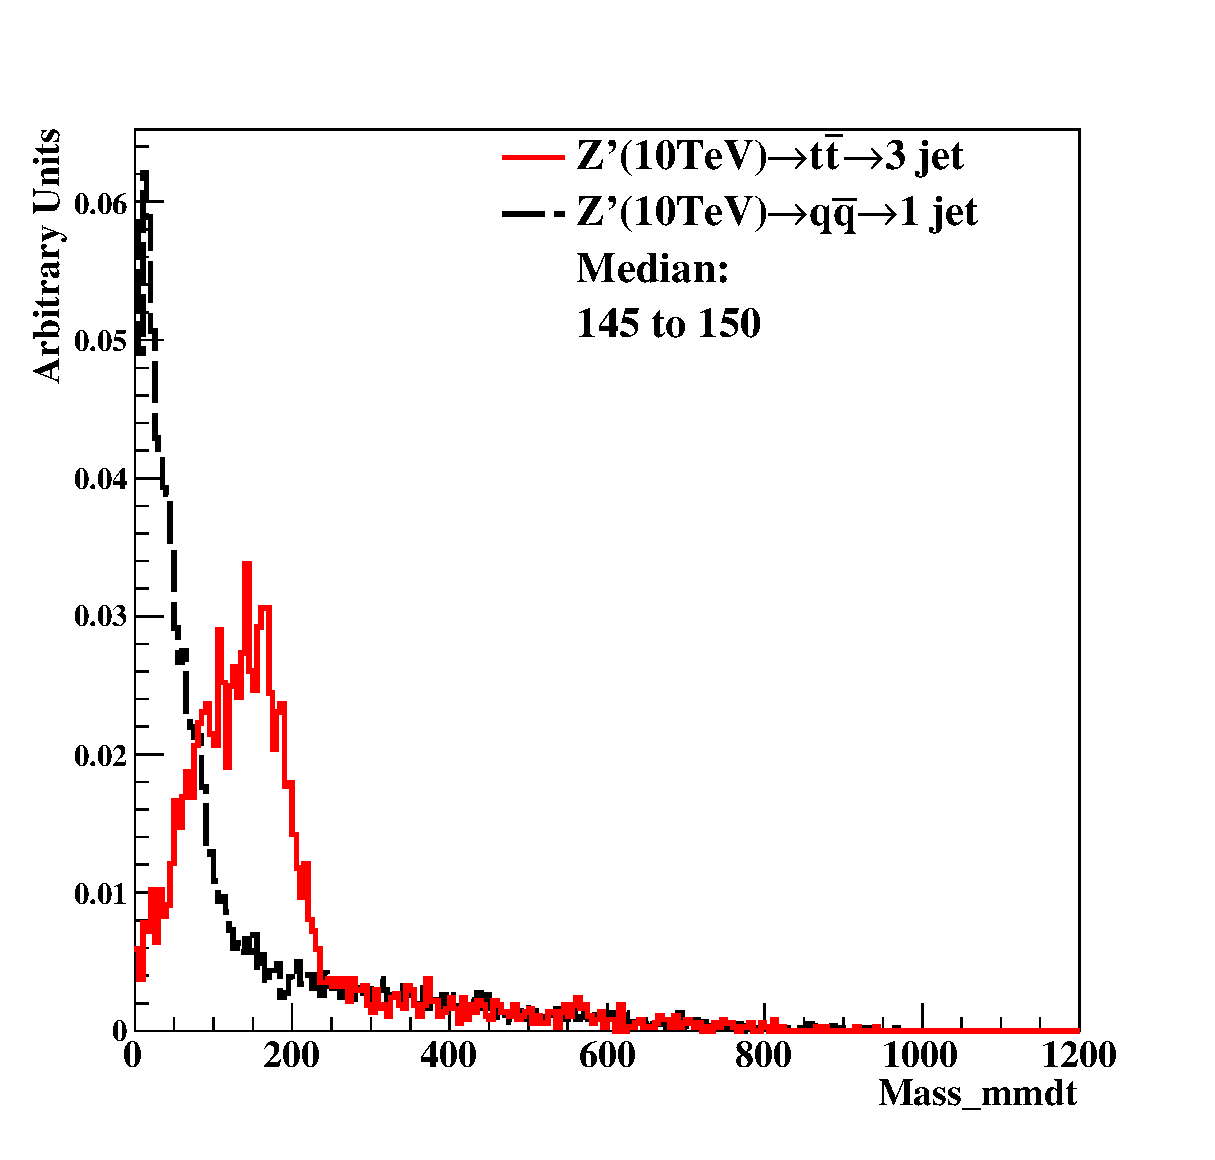
\includegraphics[width=0.22\textwidth]{figs/Dis_cluster_009_mass_mmdt_tt_10tev_04_tt.eps}
   }
   \subfigure[20TeV at 20$\times$20(cm$\times$cm) in cluster] {
   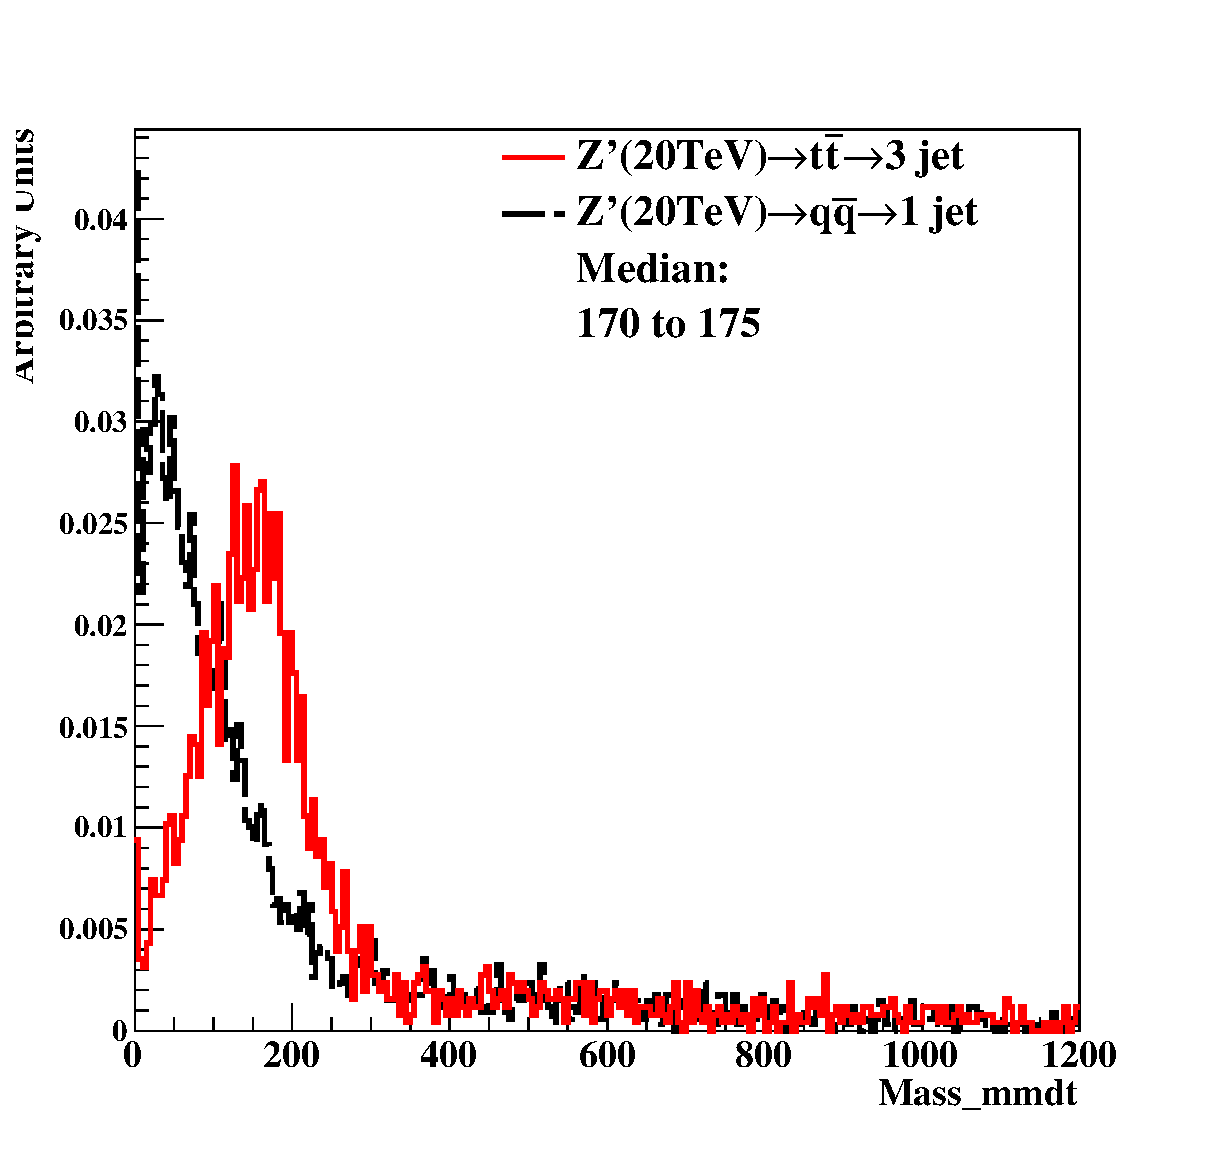
\includegraphics[width=0.22\textwidth]{figs/Dis_cluster_009_mass_mmdt_tt_20tev_04_tt.eps}\hfill
   }
      \subfigure[40TeV at 20$\times$20(cm$\times$cm) in cluster] {
   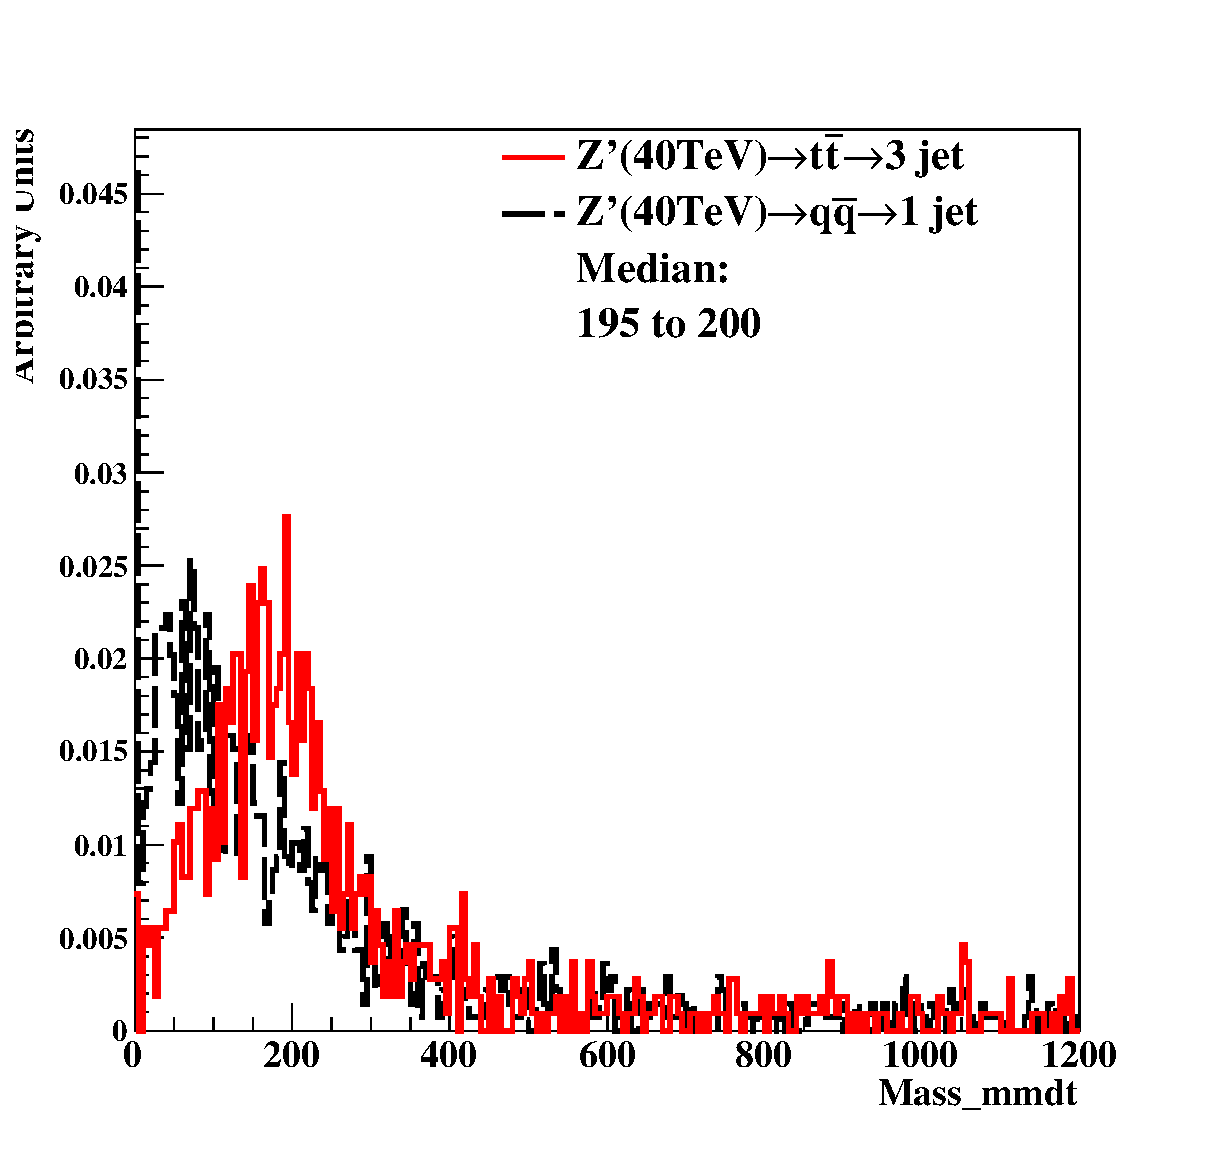
\includegraphics[width=0.22\textwidth]{figs/Dis_cluster_009_mass_mmdt_tt_40tev_04_tt.eps}\hfill
   }
   \subfigure[5TeV at 5$\times$5(cm$\times$cm) in cluster] {
   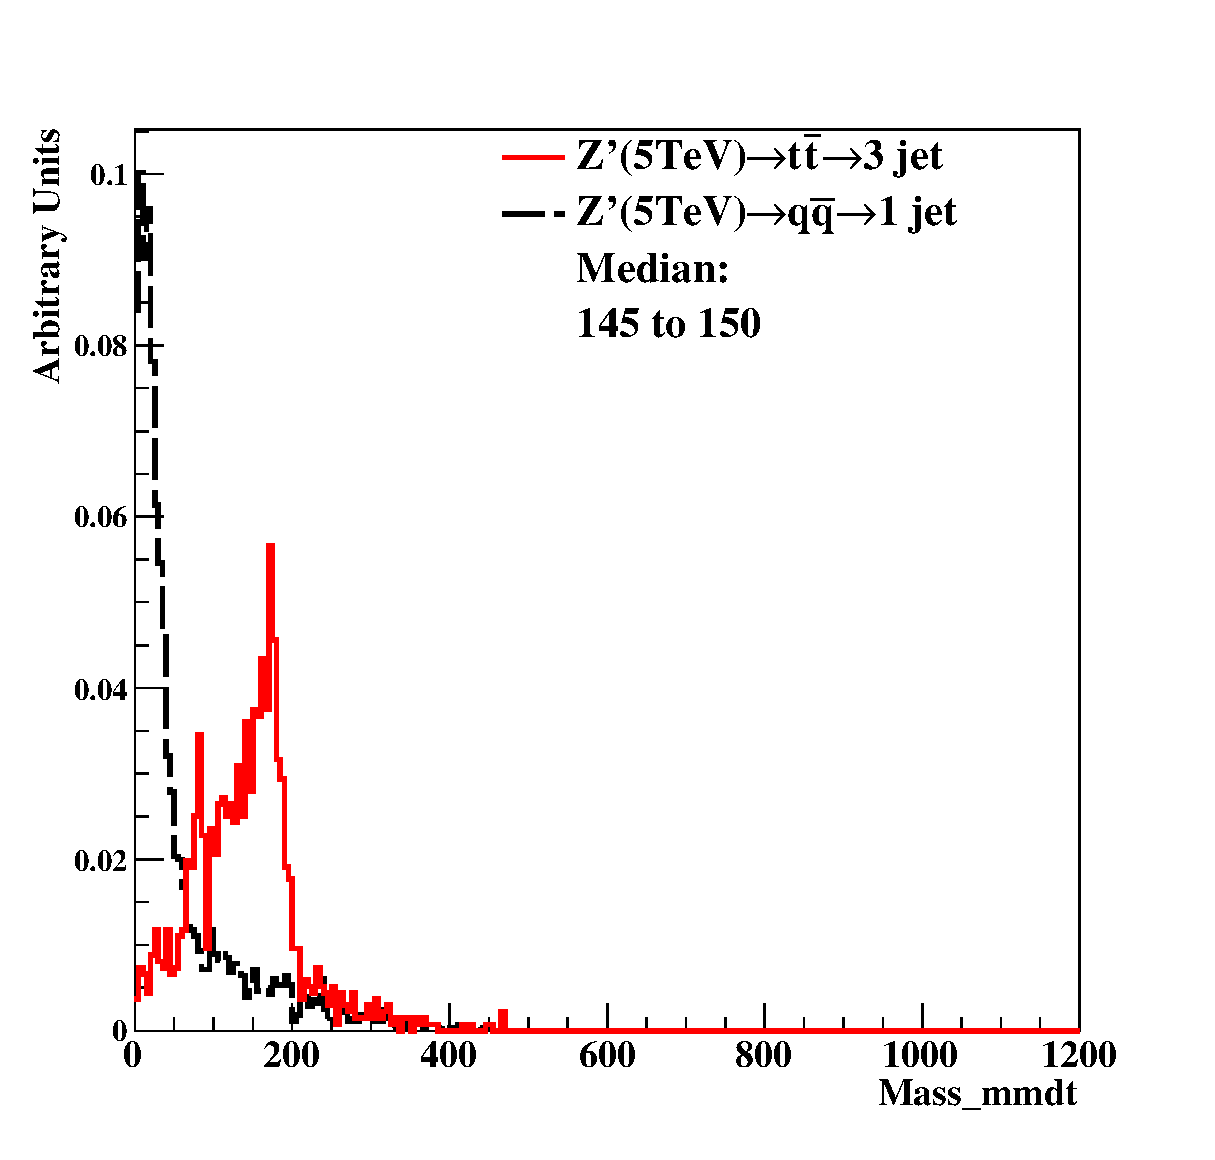
\includegraphics[width=0.22\textwidth]{figs/Dis_cluster_012_mass_mmdt_tt_5tev_04_tt.eps}\hfill
   }
    \subfigure[10TeV at 5$\times$5(cm$\times$cm) in cluster] {
   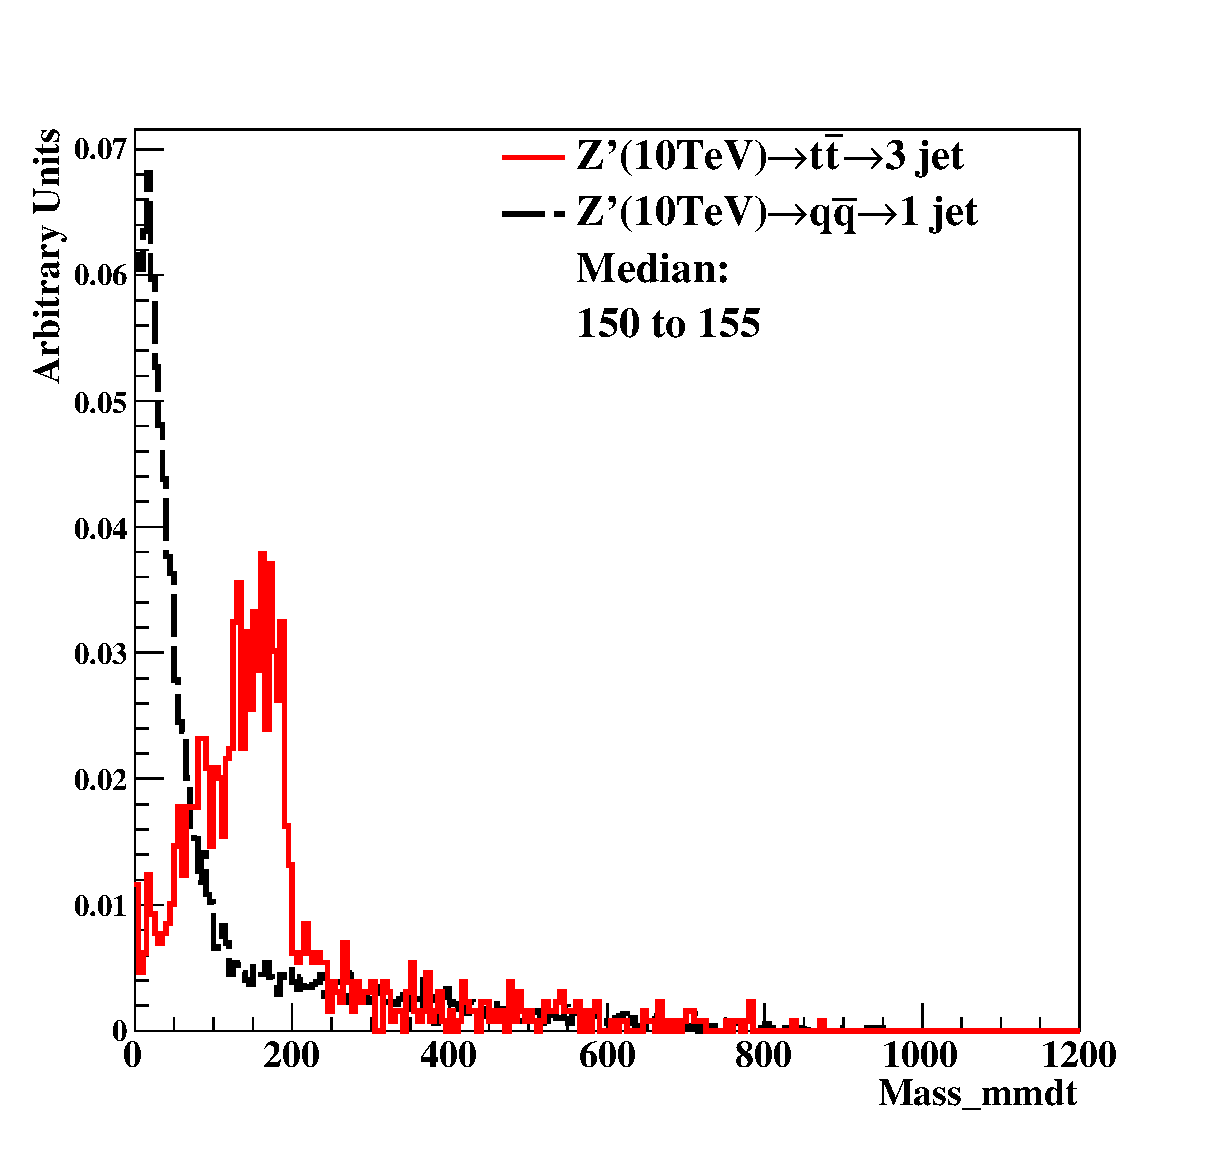
\includegraphics[width=0.22\textwidth]{figs/Dis_cluster_012_mass_mmdt_tt_10tev_04_tt.eps}
   }
   \subfigure[20TeV at 1$\times$1(cm$\times$cm) in cluster] {
   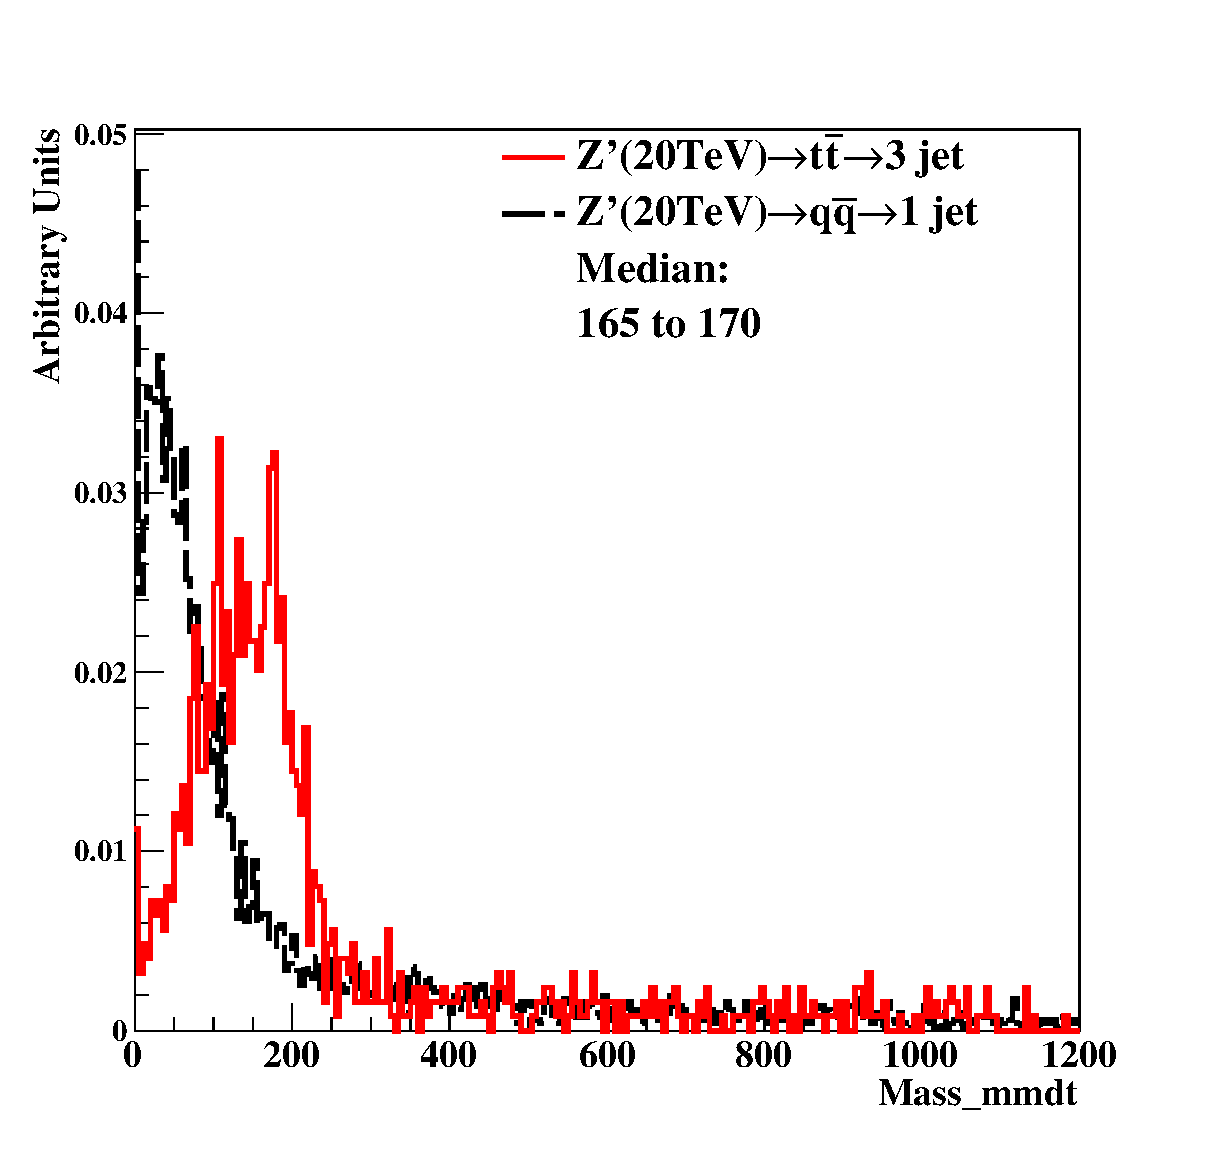
\includegraphics[width=0.22\textwidth]{figs/Dis_cluster_012_mass_mmdt_tt_20tev_04_tt.eps}\hfill
   }
      \subfigure[40TeV at 1$\times$1(cm$\times$cm) in cluster] {
   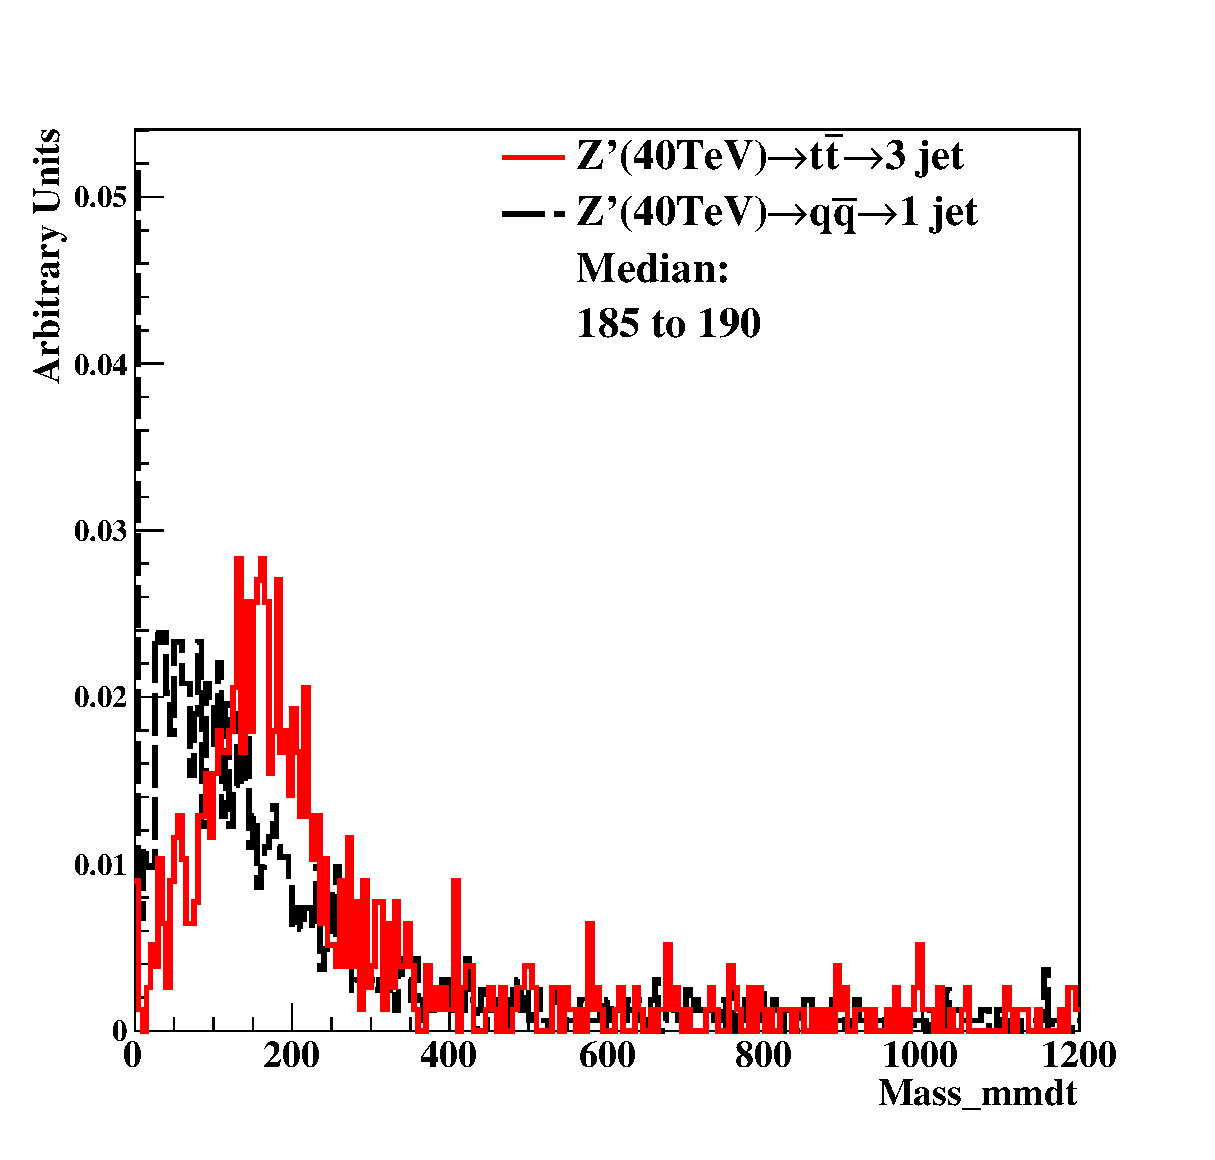
\includegraphics[width=0.22\textwidth]{figs/Dis_cluster_012_mass_mmdt_tt_40tev_04_tt.eps}
   }
\end{center}
\caption{Distributions of mass soft drop at $\beta$=0, signal=tt, in 5,10TeV energy of collision  in different detector sizes. Cell Size in 20$\times$20, 5$\times$5, and 1$\times$1(cm$\times$cm) are shown here.}
\label{fig:cluster_tau21_tau32}
\end{figure}

\begin{figure}
\begin{center}
  \subfigure[Central at Median($20\times20$=150,$5\times5$=150,$1\times1$=150) change width in cluster at 5TeV] {
  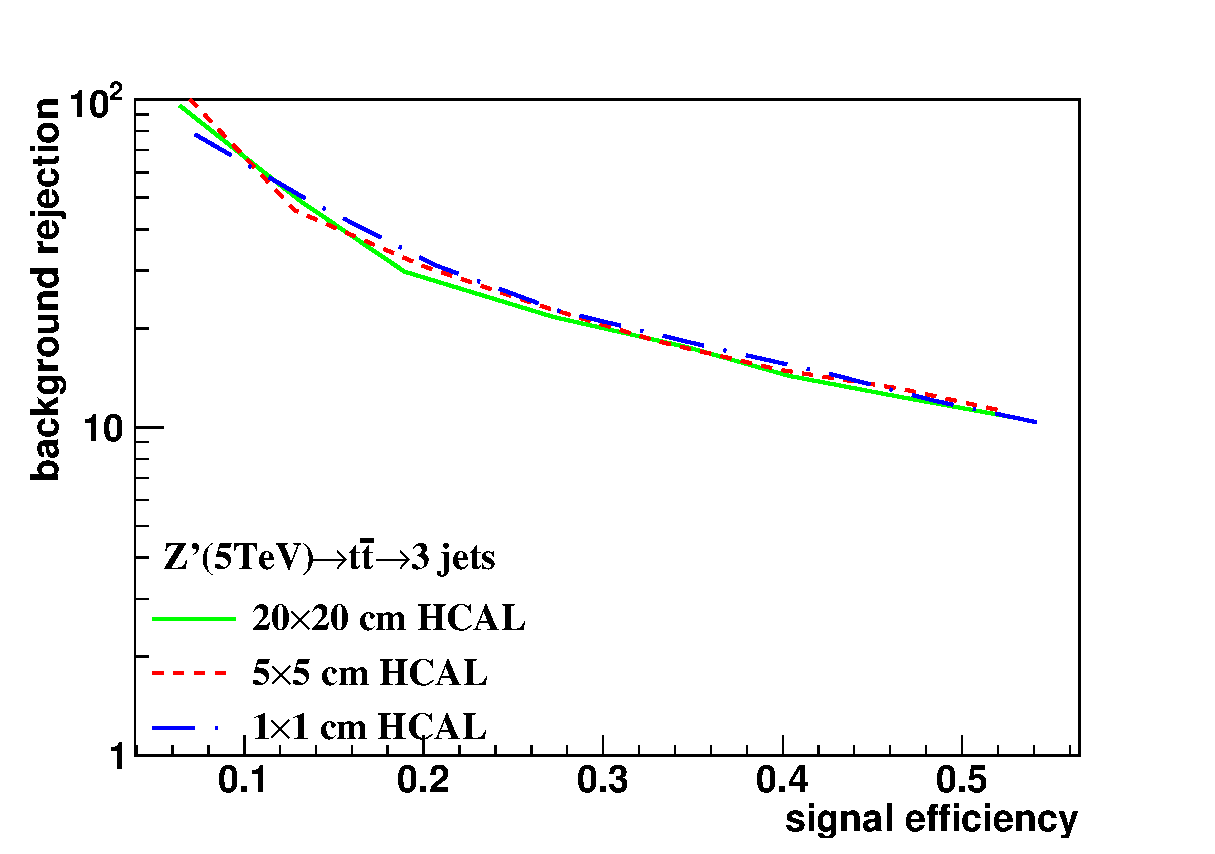
\includegraphics[width=0.43\textwidth]{figs/A_Cluster_mass_mmdt_5tev_eff_1_central_fix_tt_qq_log.eps}
  }
  \subfigure[Central at Median($20\times20$=155,$5\times5$=150,$1\times1$=155) change width in cluster at 10TeV] {
  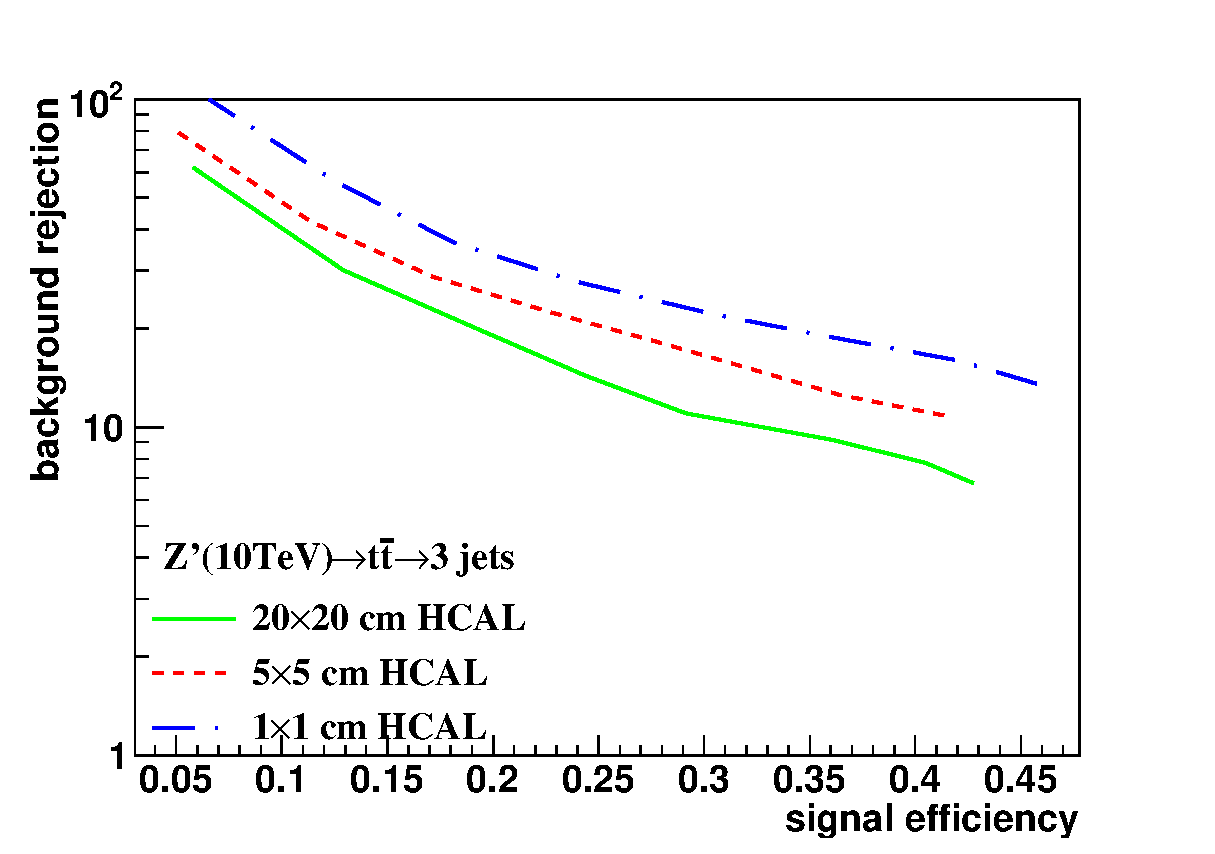
\includegraphics[width=0.43\textwidth]{figs/A_Cluster_mass_mmdt_10tev_eff_1_central_fix_tt_qq_log.eps}
  }
 \subfigure[Central at Median($20\times20$=165,$5\times5$=175,$1\times1$=170) change width in cluster at 20TeV] {
 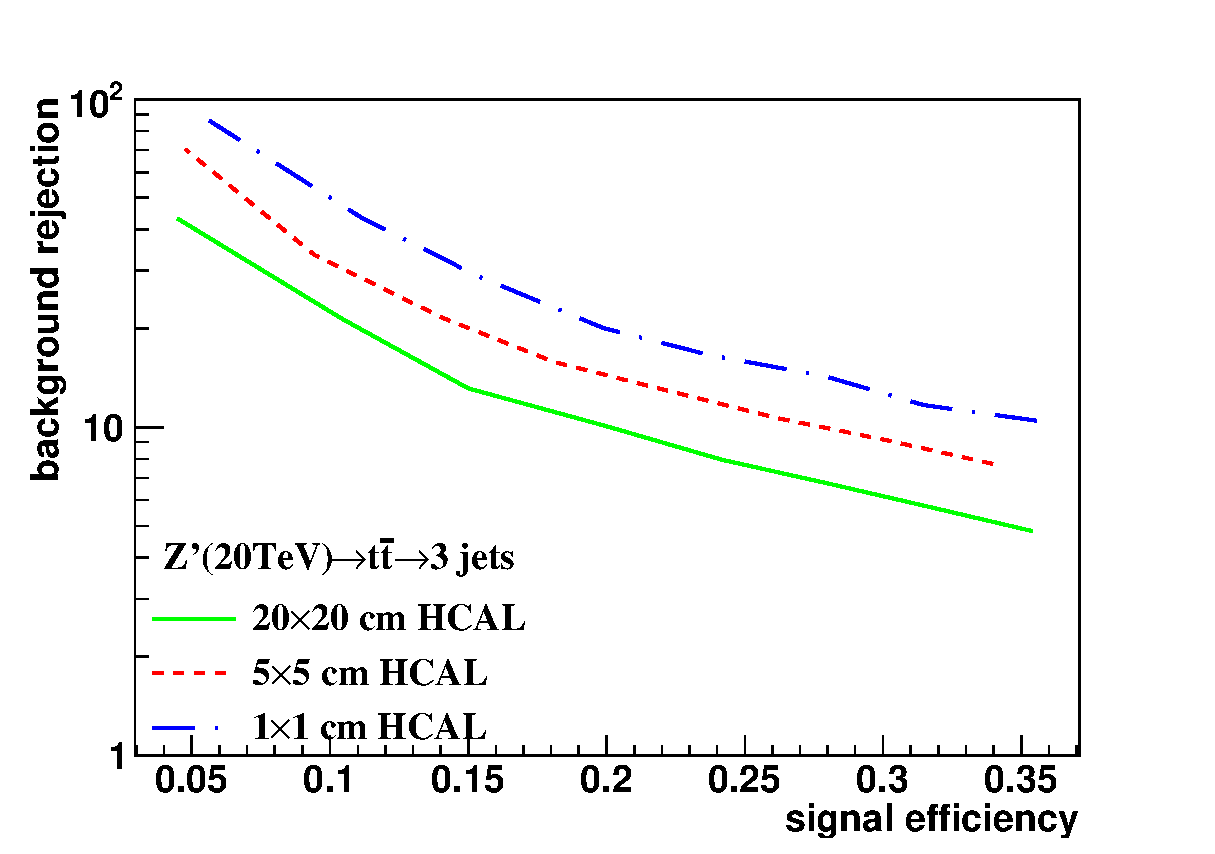
\includegraphics[width=0.43\textwidth]{figs/A_Cluster_mass_mmdt_20tev_eff_1_central_fix_tt_qq_log.eps}
 }
 \subfigure[Central at Median($20\times20$=190,$5\times5$=200,$1\times1$=190) change width in cluster at 40TeV] {
 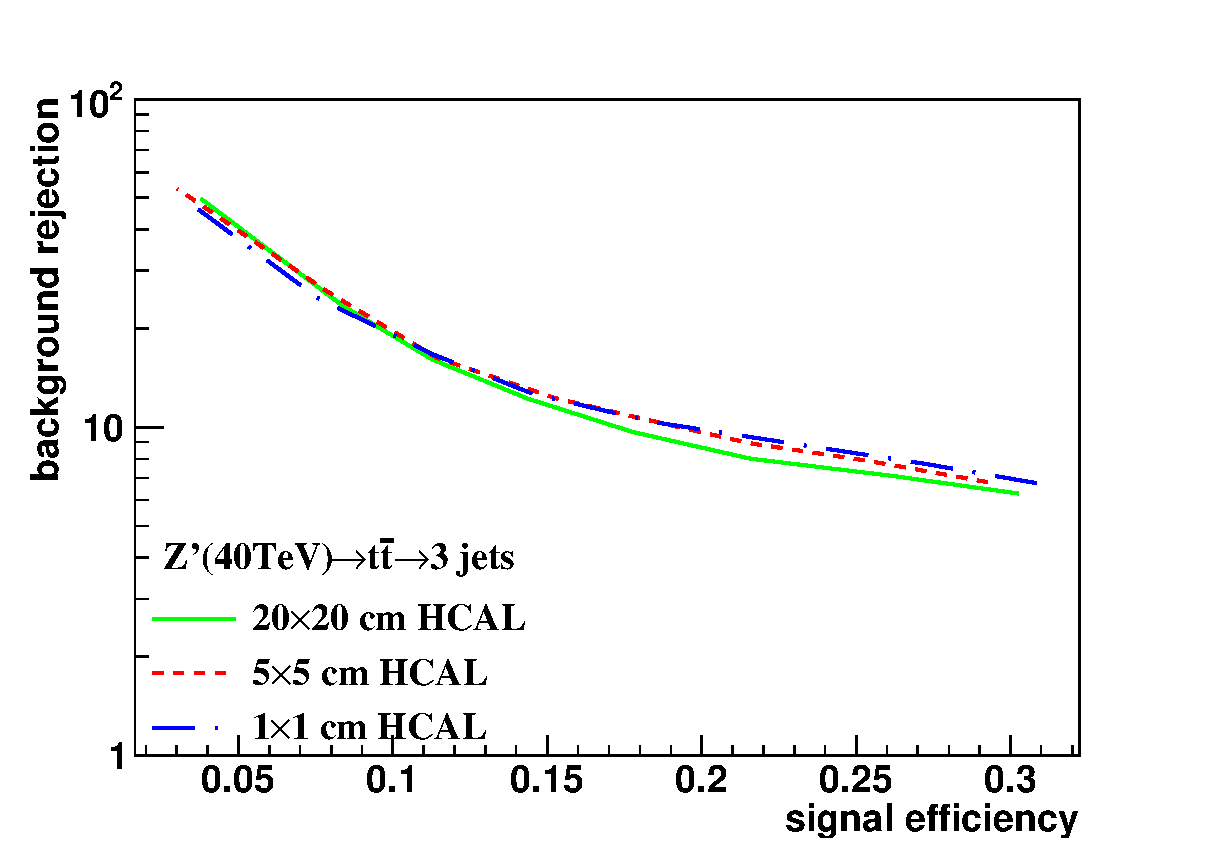
\includegraphics[width=0.43\textwidth]{figs/A_Cluster_mass_mmdt_40tev_eff_1_central_fix_tt_qq_log.eps}
 }
\end{center}
\caption{study of "fix central and change width" in mass soft drop at $\beta$=0, signal=tt, in 5, 10, 20, 40TeV energy of collision  in different detector sizes. Cell Size in 20$\times$20, 5$\times$5, and 1$\times$1(cm$\times$cm) are shown in each picture.}
\label{fig:cluster_tau21_tau32}
\end{figure}


\begin{figure}
\begin{center}
   \subfigure[5TeV at 20$\times$20(cm$\times$cm) in cluster] {
   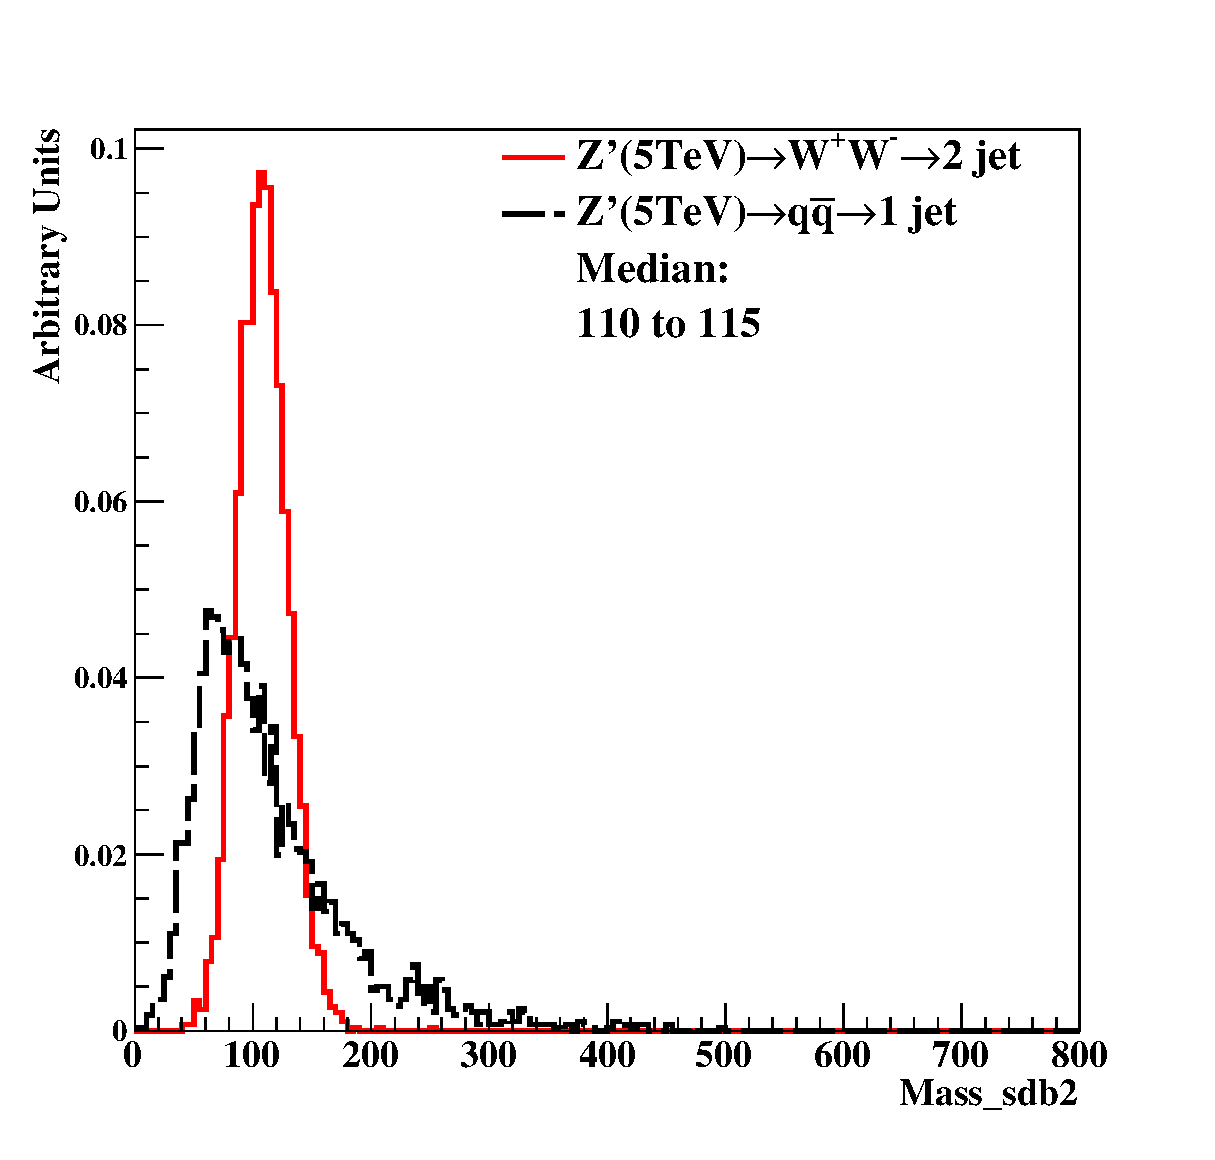
\includegraphics[width=0.22\textwidth]{figs/Dis_cluster_010_mass_sdb2_ww_5tev_04_800.eps}
   }
      \subfigure[10TeV at 20$\times$20(cm$\times$cm) in cluster] {
   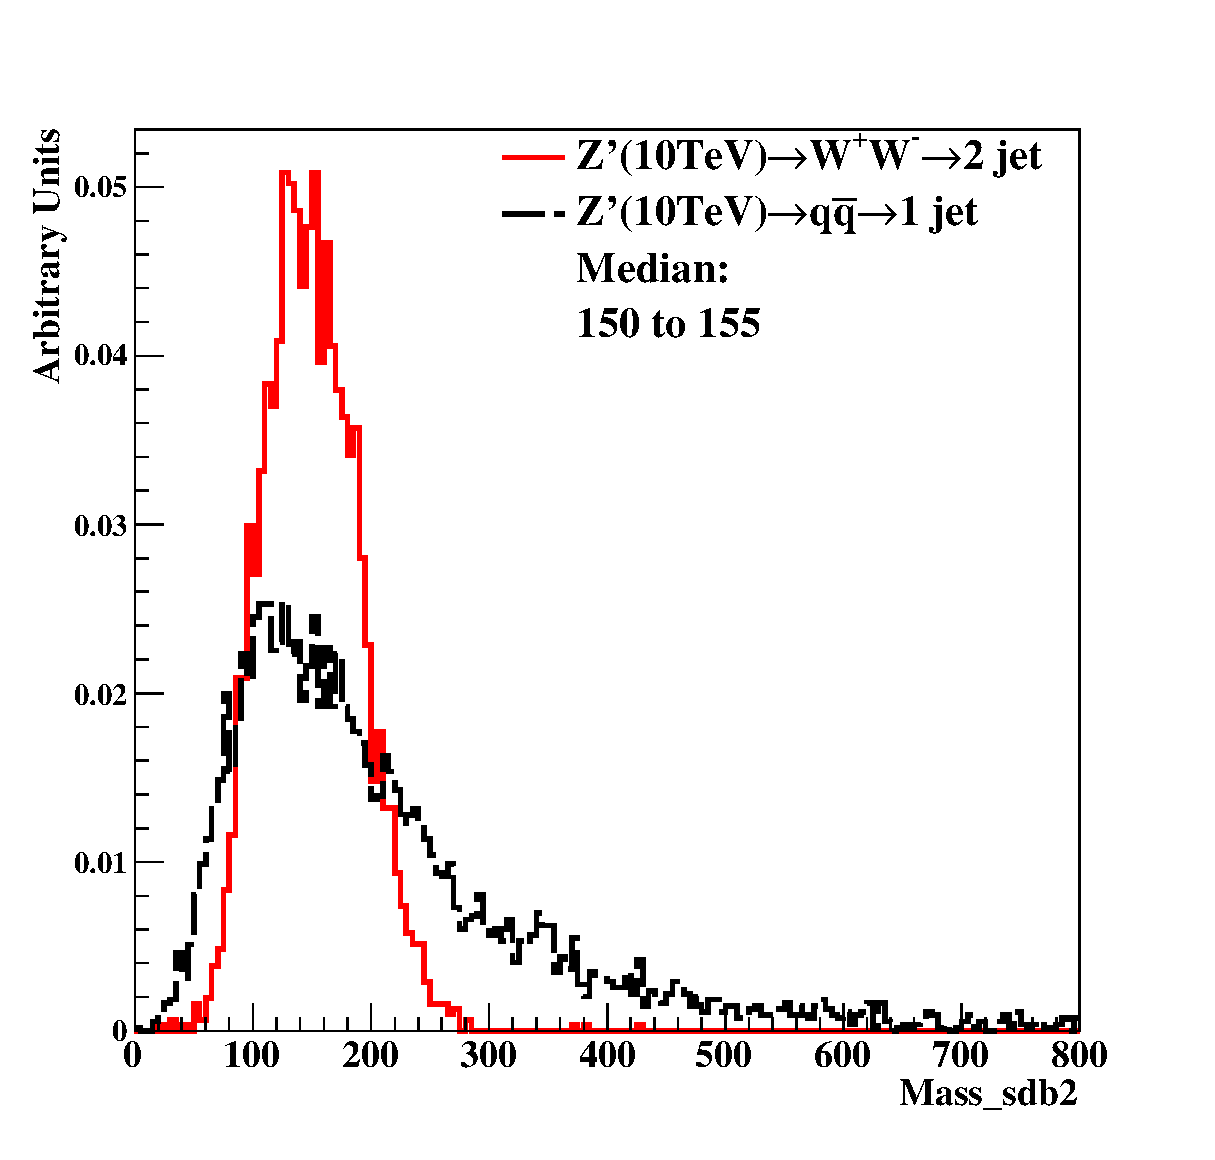
\includegraphics[width=0.22\textwidth]{figs/Dis_cluster_010_mass_sdb2_ww_10tev_04_800.eps}
   }
   \subfigure[20TeV at 20$\times$20(cm$\times$cm) in cluster] {
   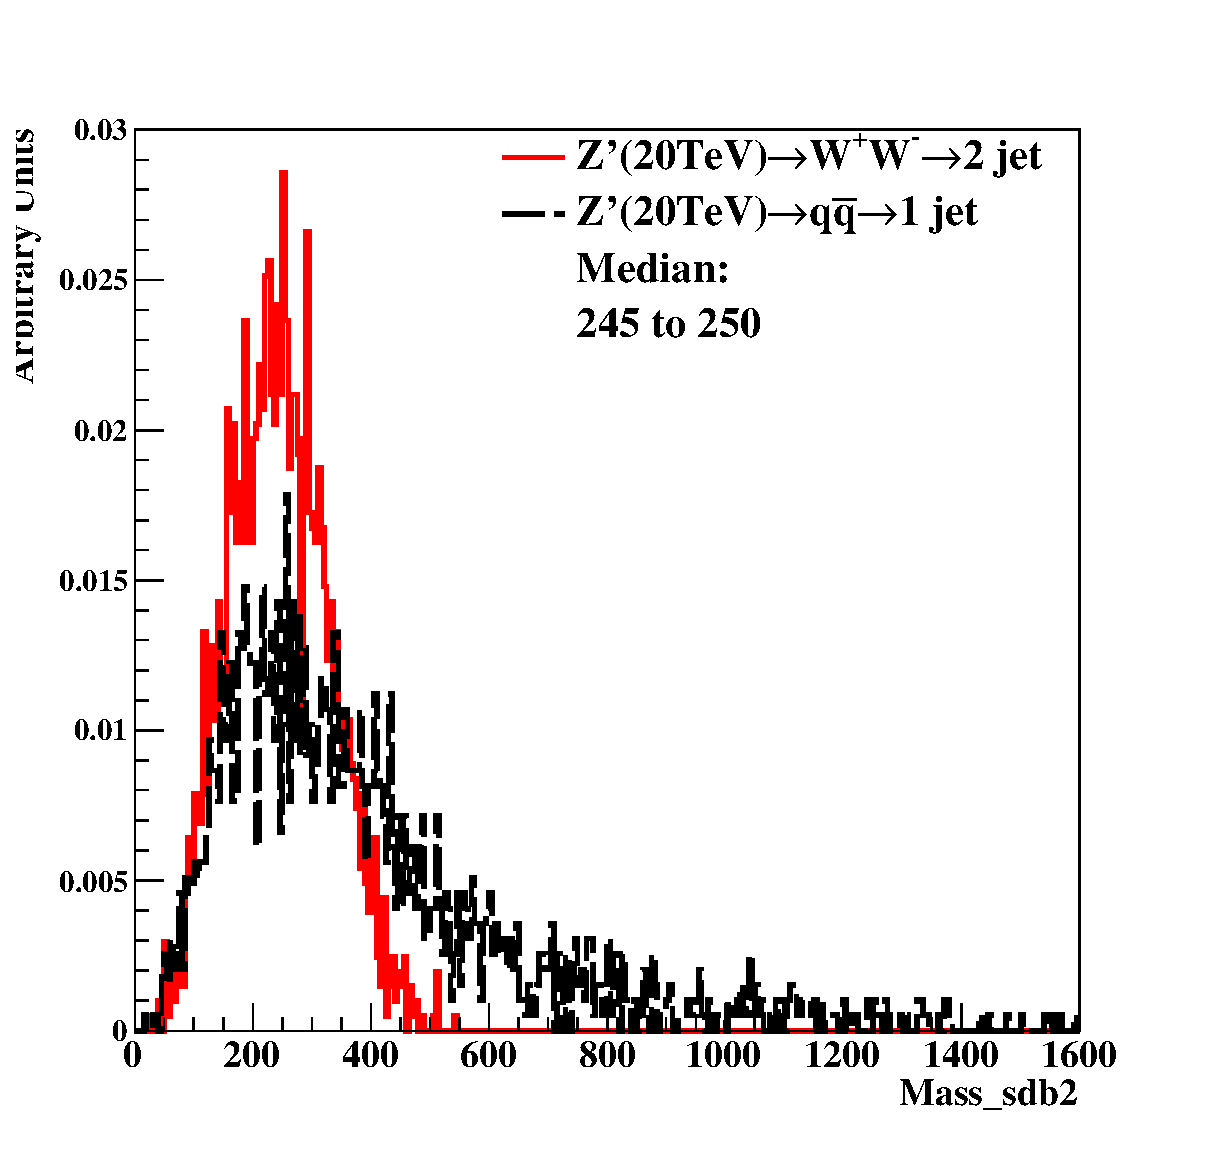
\includegraphics[width=0.22\textwidth]{figs/Dis_cluster_010_mass_sdb2_ww_20tev_04_1600.eps}
   }
    \subfigure[40TeV at 20$\times$20(cm$\times$cm) in cluster] {
   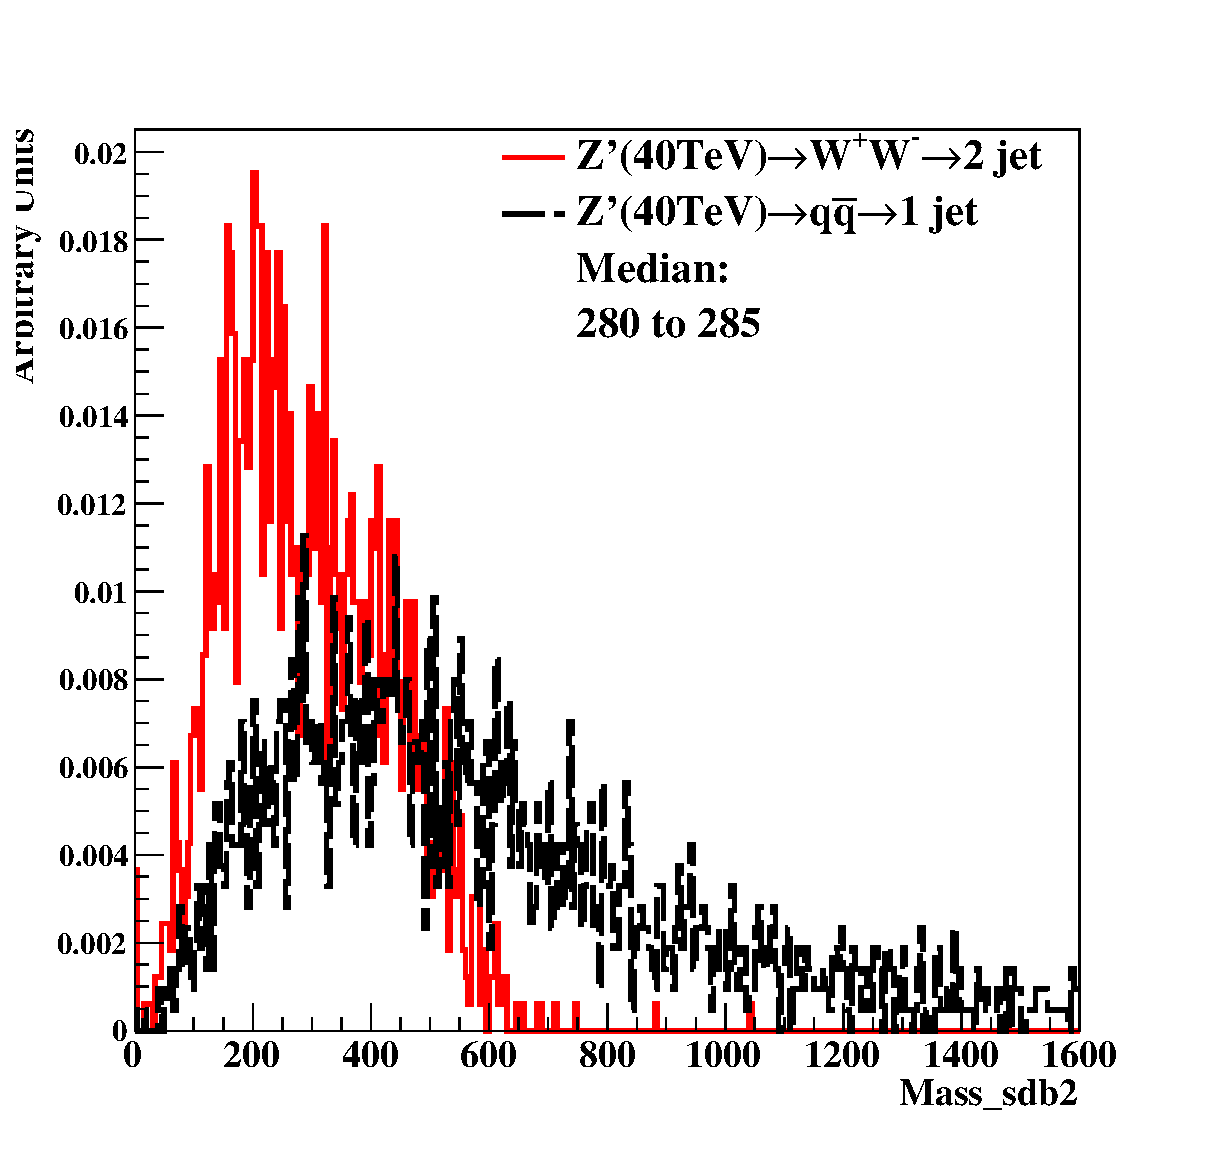
\includegraphics[width=0.22\textwidth]{figs/Dis_cluster_010_mass_sdb2_ww_40tev_04_1600.eps}
   }
   \subfigure[5TeV at 5$\times$5(cm$\times$cm) in cluster] {
   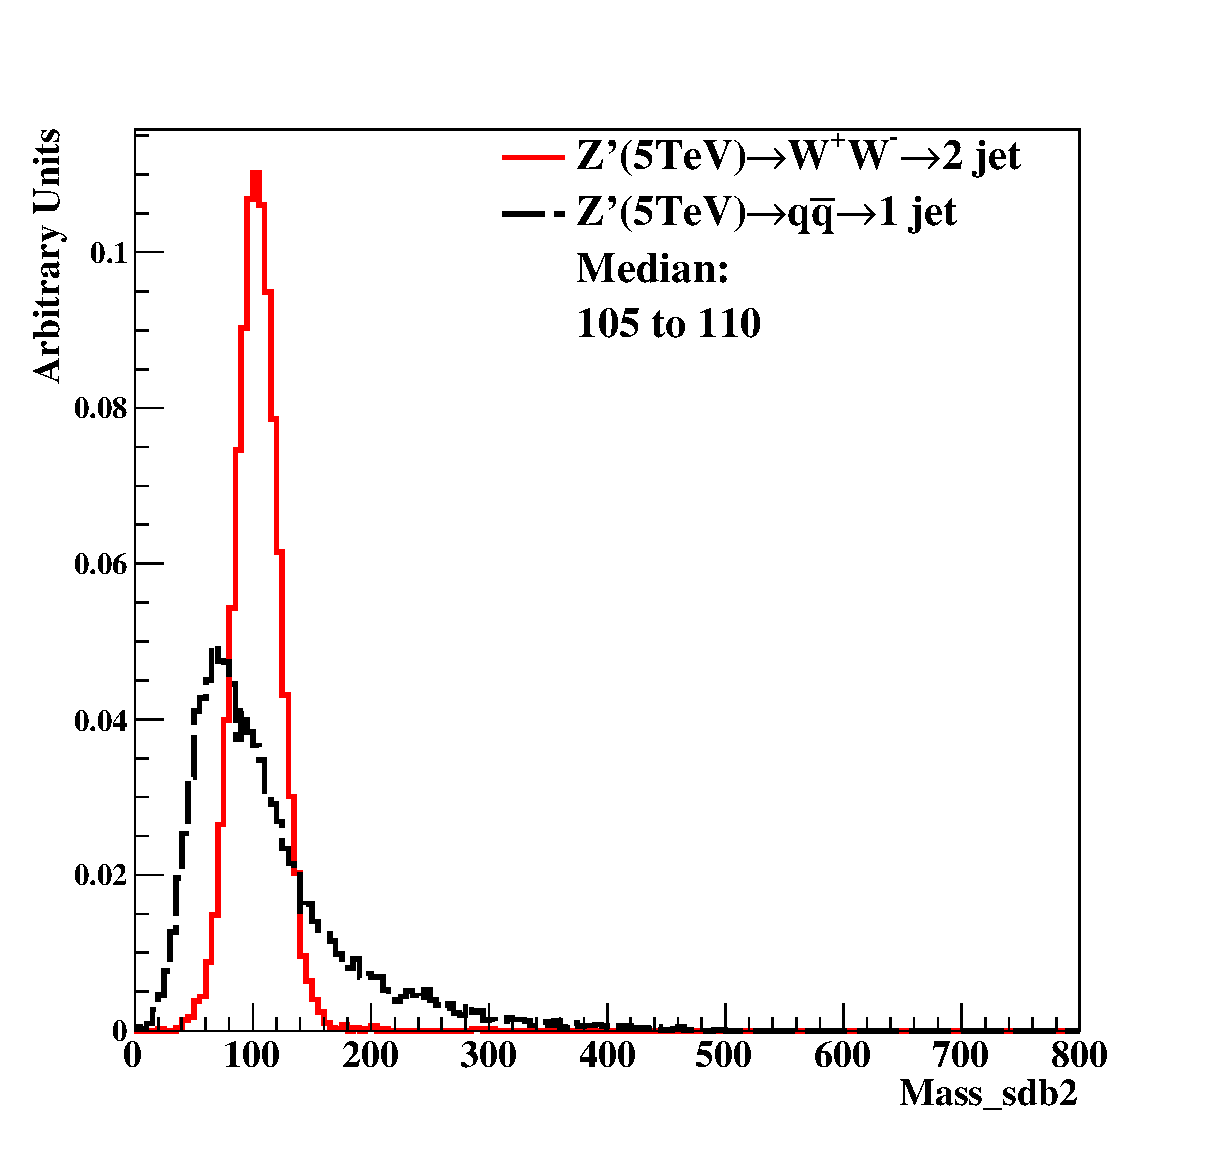
\includegraphics[width=0.22\textwidth]{figs/Dis_cluster_009_mass_sdb2_ww_5tev_04_800.eps}
   }
   \subfigure[10TeV at 5$\times$5(cm$\times$cm) in cluster] {
   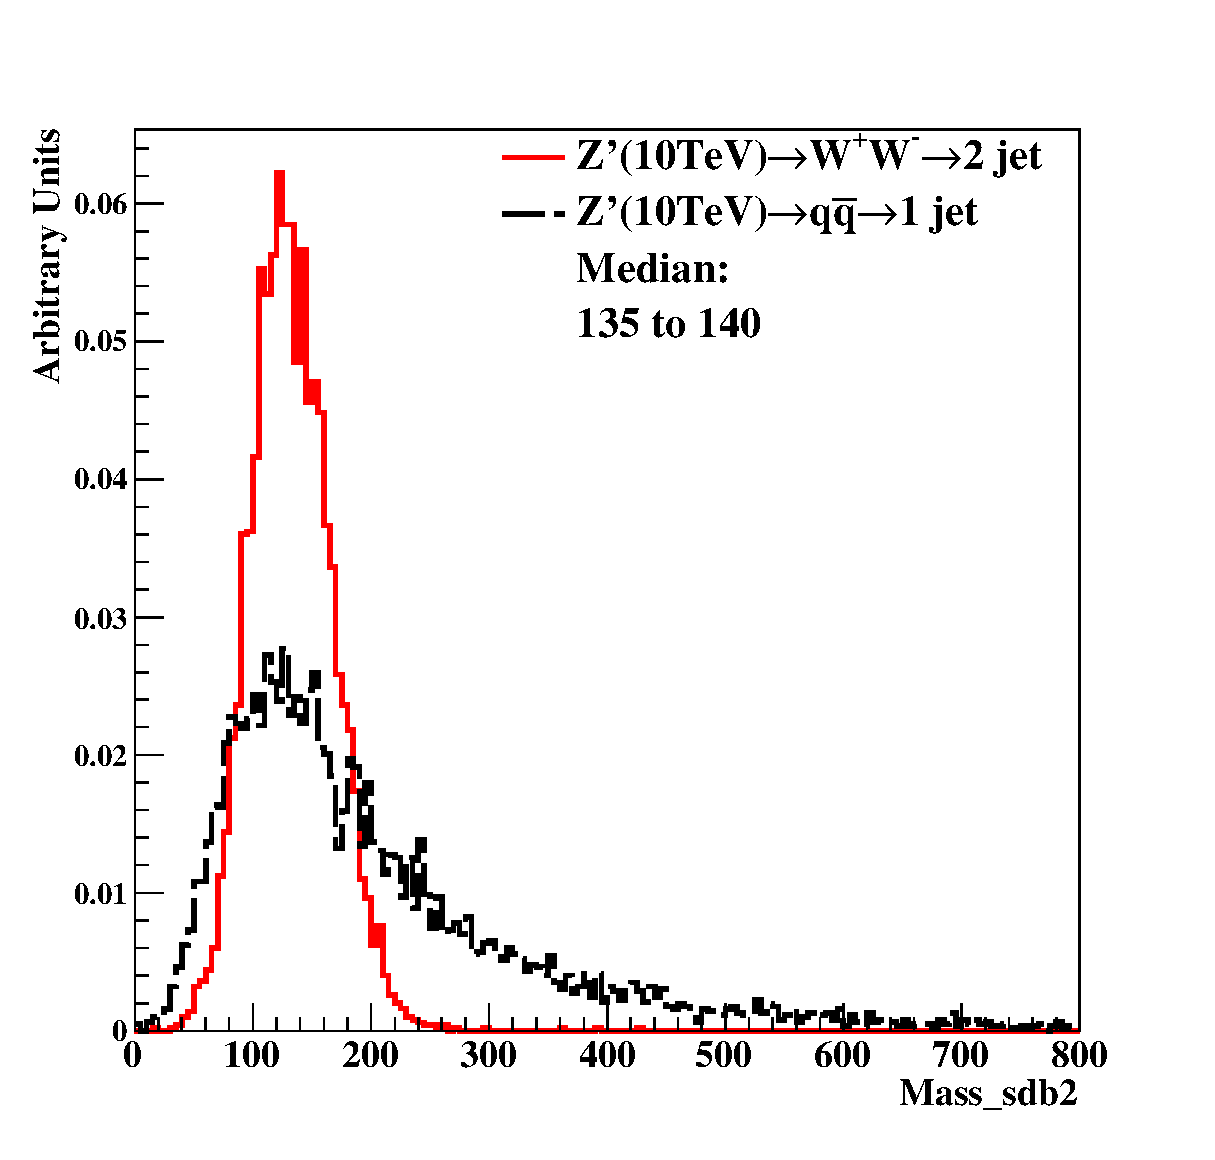
\includegraphics[width=0.22\textwidth]{figs/Dis_cluster_009_mass_sdb2_ww_10tev_04_800.eps}
   }
    \subfigure[20TeV at 5$\times$5(cm$\times$cm) in cluster] {
   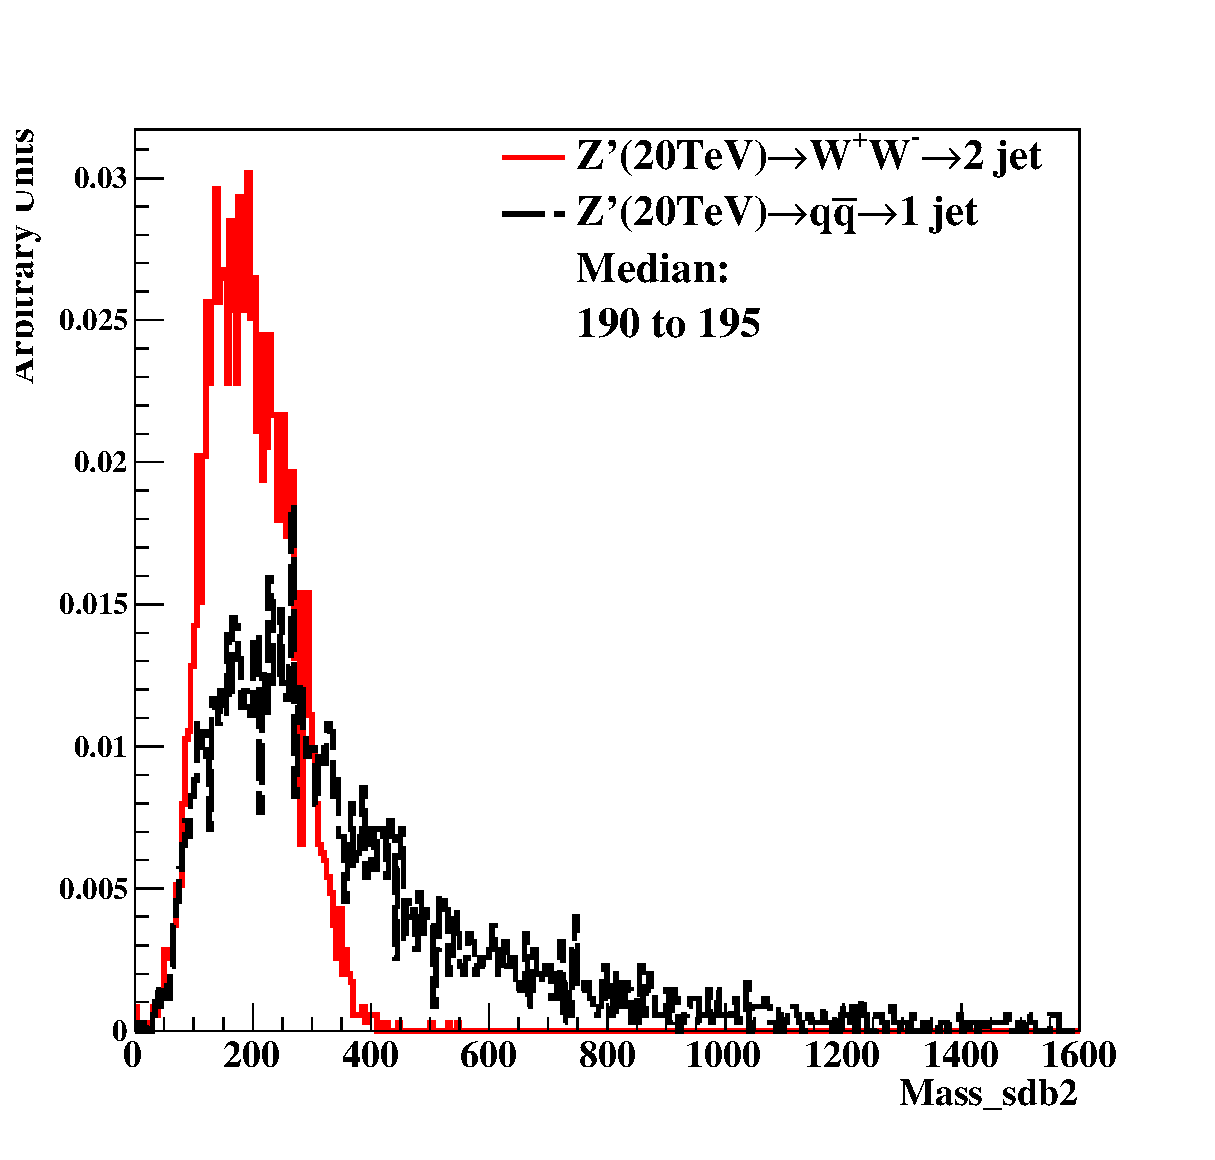
\includegraphics[width=0.22\textwidth]{figs/Dis_cluster_009_mass_sdb2_ww_20tev_04_1600.eps}\hfill
   }
      \subfigure[40TeV at 5$\times$5(cm$\times$cm) in cluster] {
   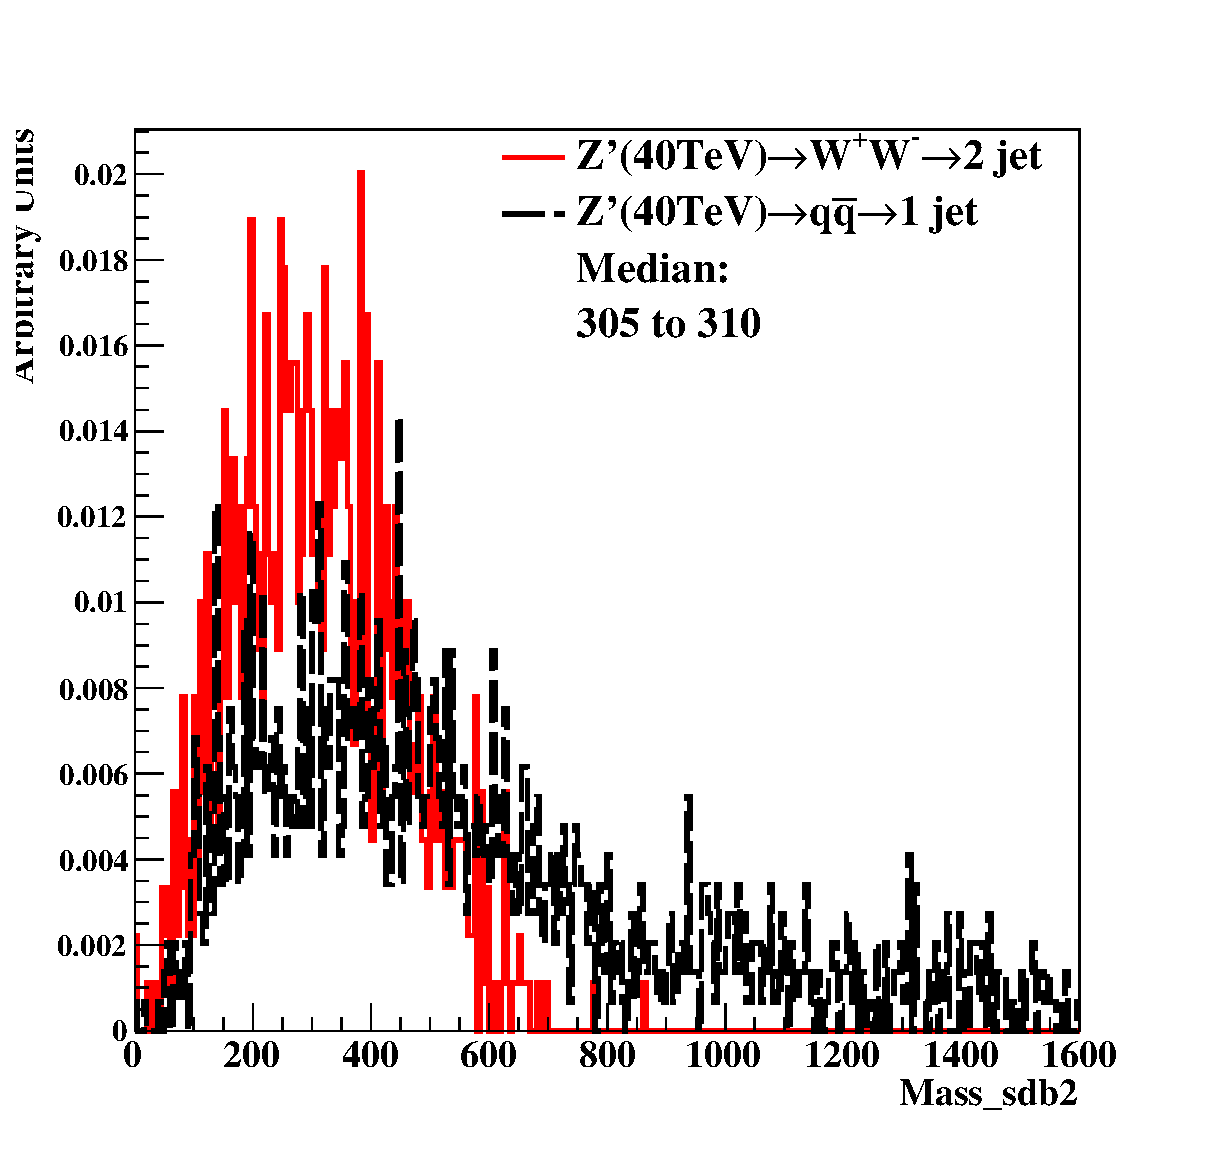
\includegraphics[width=0.22\textwidth]{figs/Dis_cluster_009_mass_sdb2_ww_40tev_04_1600.eps}\hfill
   }
   \subfigure[5TeV at 1$\times$1(cm$\times$cm) in cluster] {
   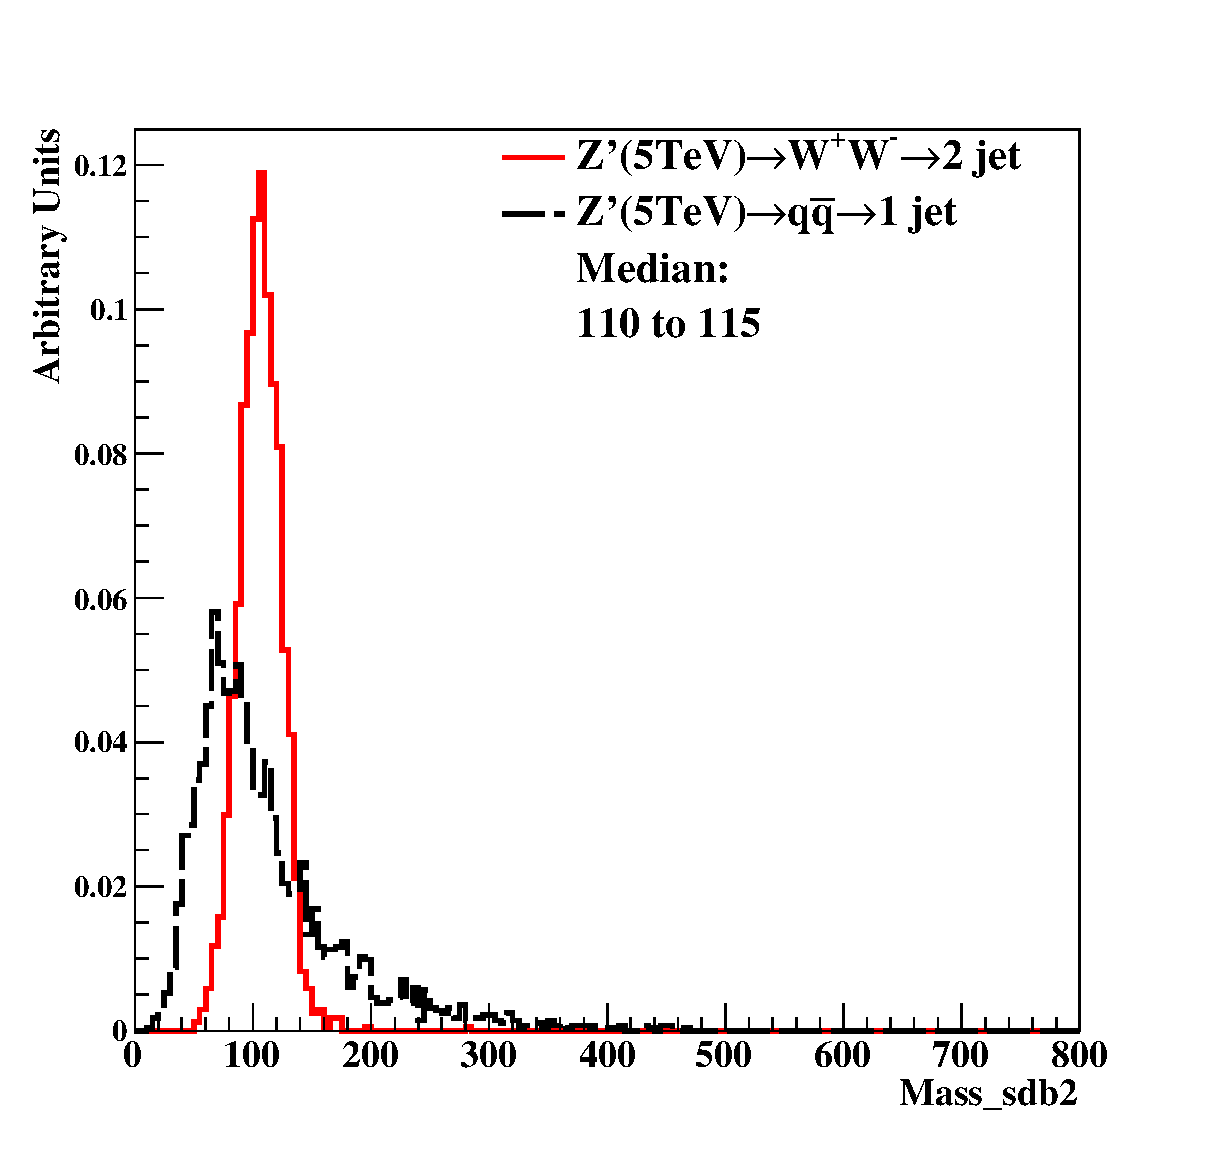
\includegraphics[width=0.22\textwidth]{figs/Dis_cluster_012_mass_sdb2_ww_5tev_04_800.eps}\hfill
   }
    \subfigure[10TeV at 1$\times$1(cm$\times$cm) in cluster] {
   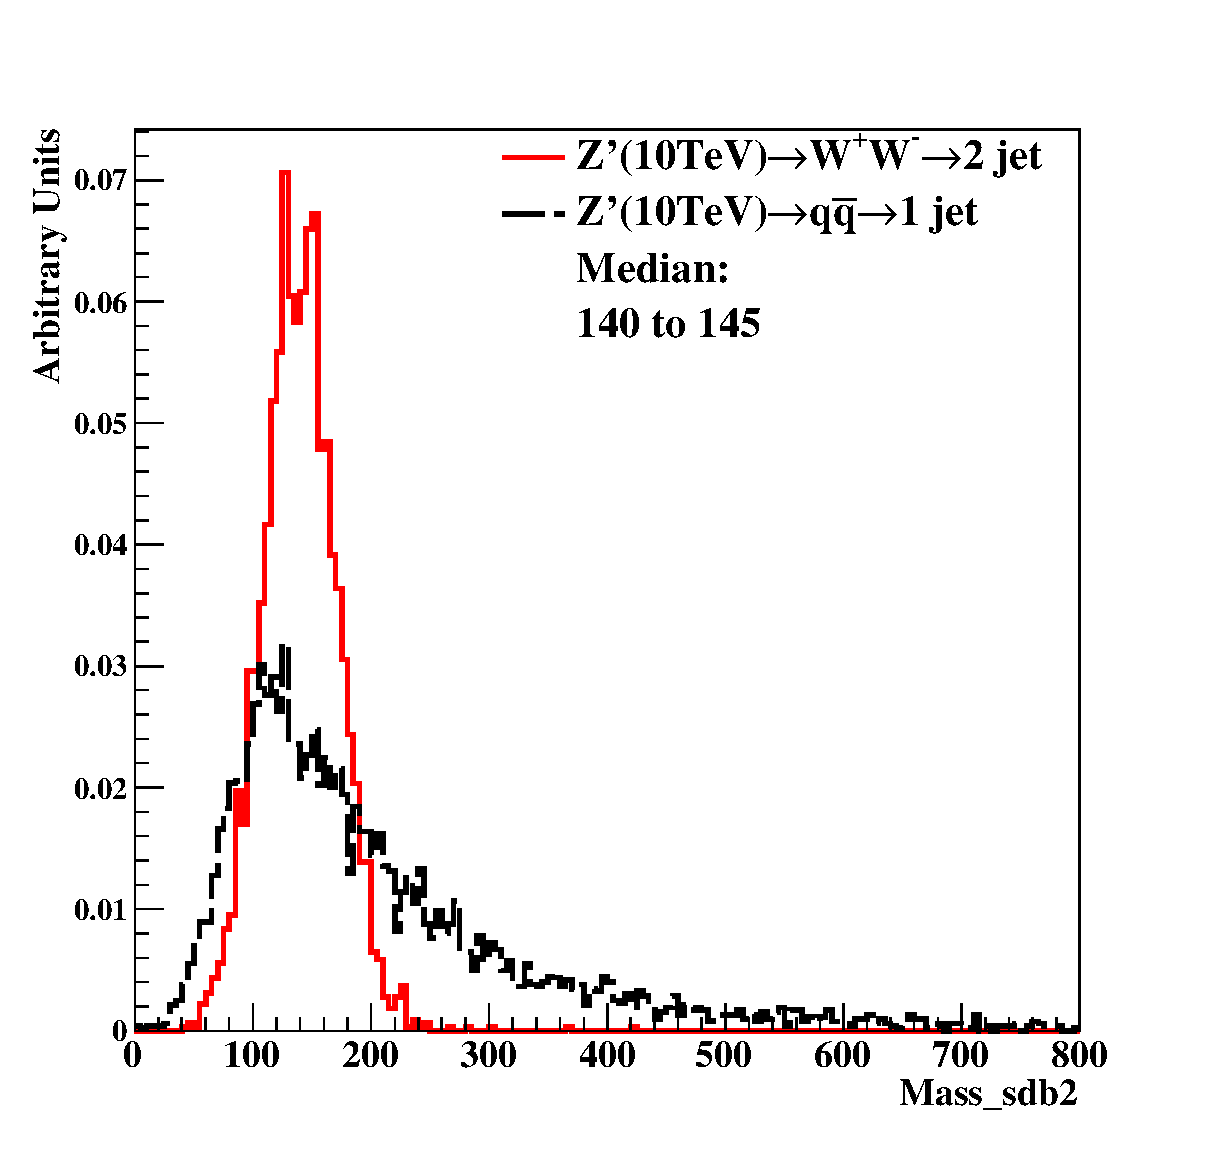
\includegraphics[width=0.22\textwidth]{figs/Dis_cluster_012_mass_sdb2_ww_10tev_04_800.eps}
   }
   \subfigure[20TeV at 1$\times$1(cm$\times$cm) in cluster] {
   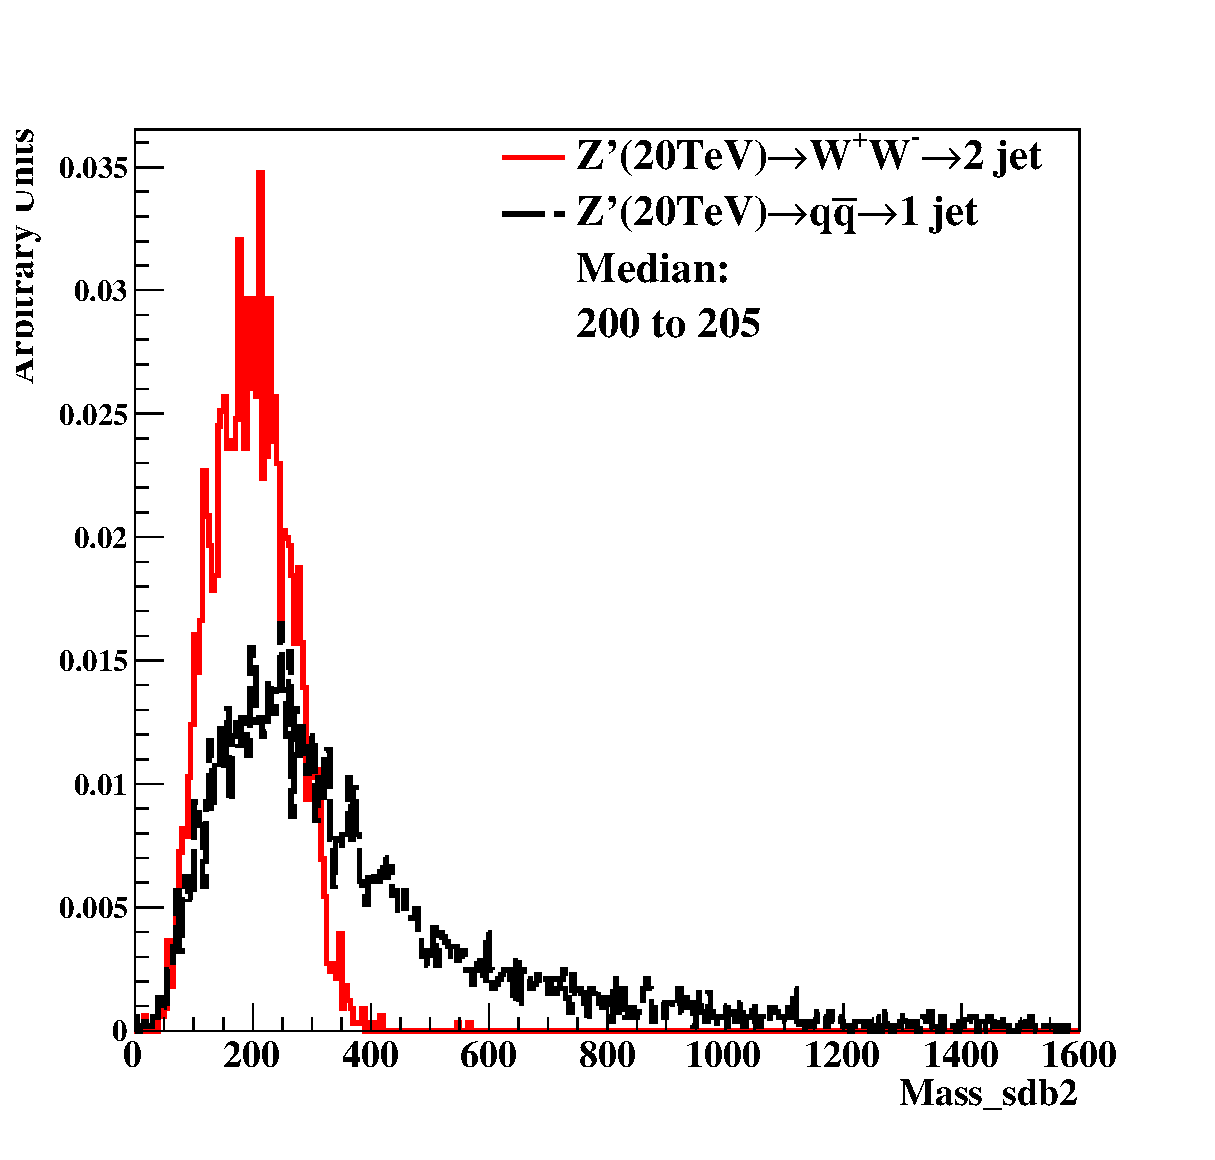
\includegraphics[width=0.22\textwidth]{figs/Dis_cluster_012_mass_sdb2_ww_20tev_04_1600.eps}\hfill
   }
      \subfigure[40TeV at 1$\times$1(cm$\times$cm) in cluster] {
   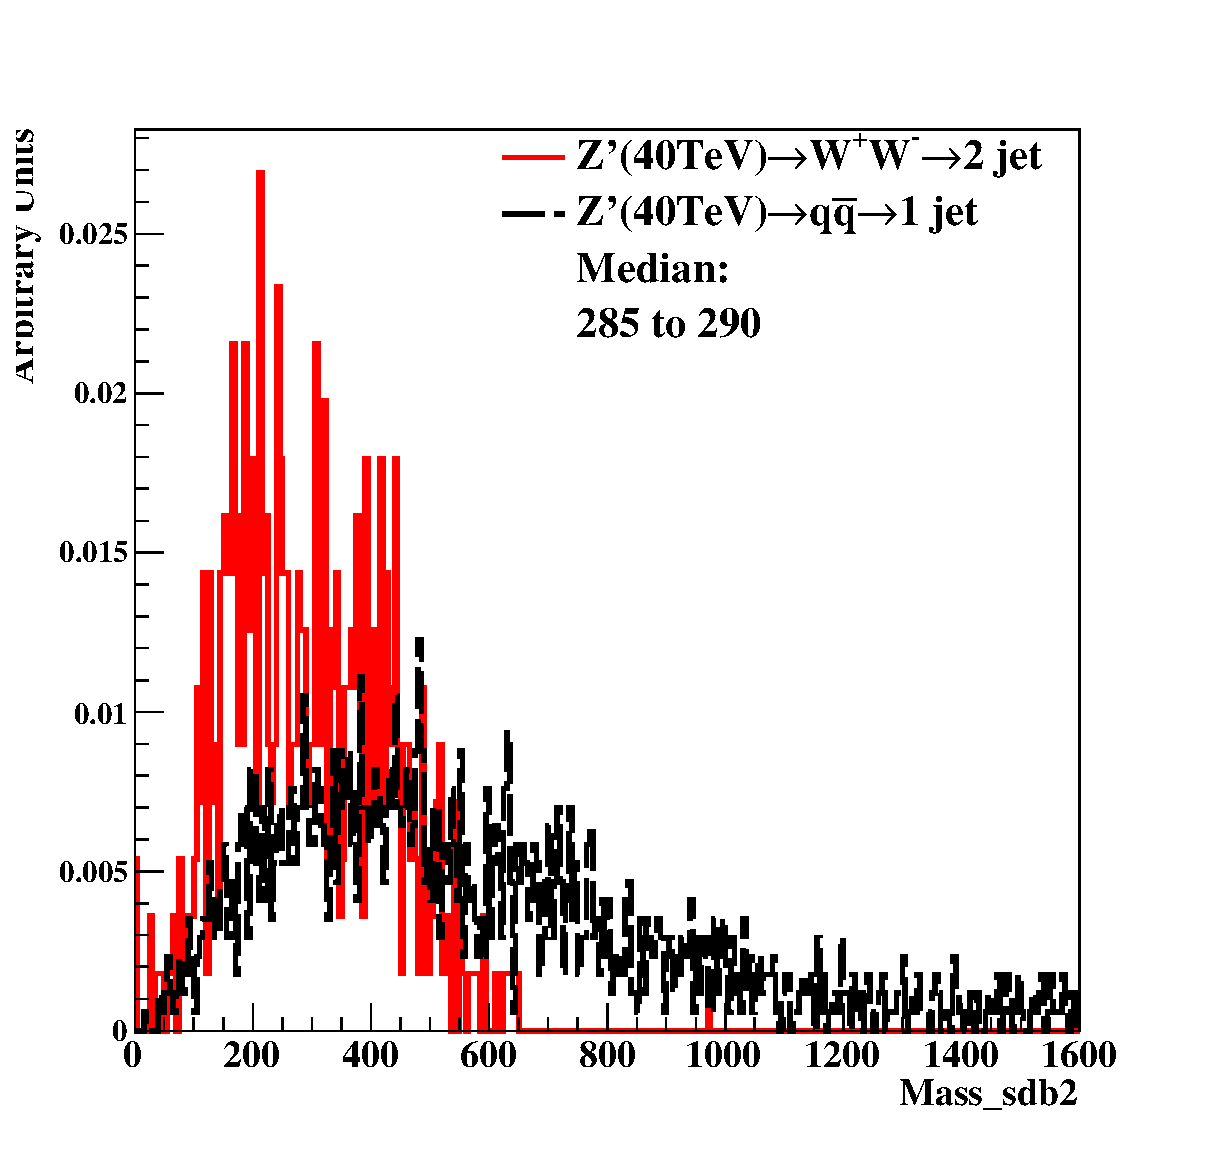
\includegraphics[width=0.22\textwidth]{figs/Dis_cluster_012_mass_sdb2_ww_40tev_04_1600.eps}
   }
\end{center}
\caption{Distributions of mass soft drop at $\beta$=2, signal=ww, in 5,10TeV energy of collision  in different detector sizes. Cell Size in 20$\times$20, 5$\times$5, and 1$\times$1(cm$\times$cm) are shown here.}
\label{fig:cluster_tau21_tau32}
\end{figure}


\begin{figure}
\begin{center}
  \subfigure[Central at Median($20\times20$=115,$5\times5$=110,$1\times1$=115) change width in cluster at 5TeV] {
  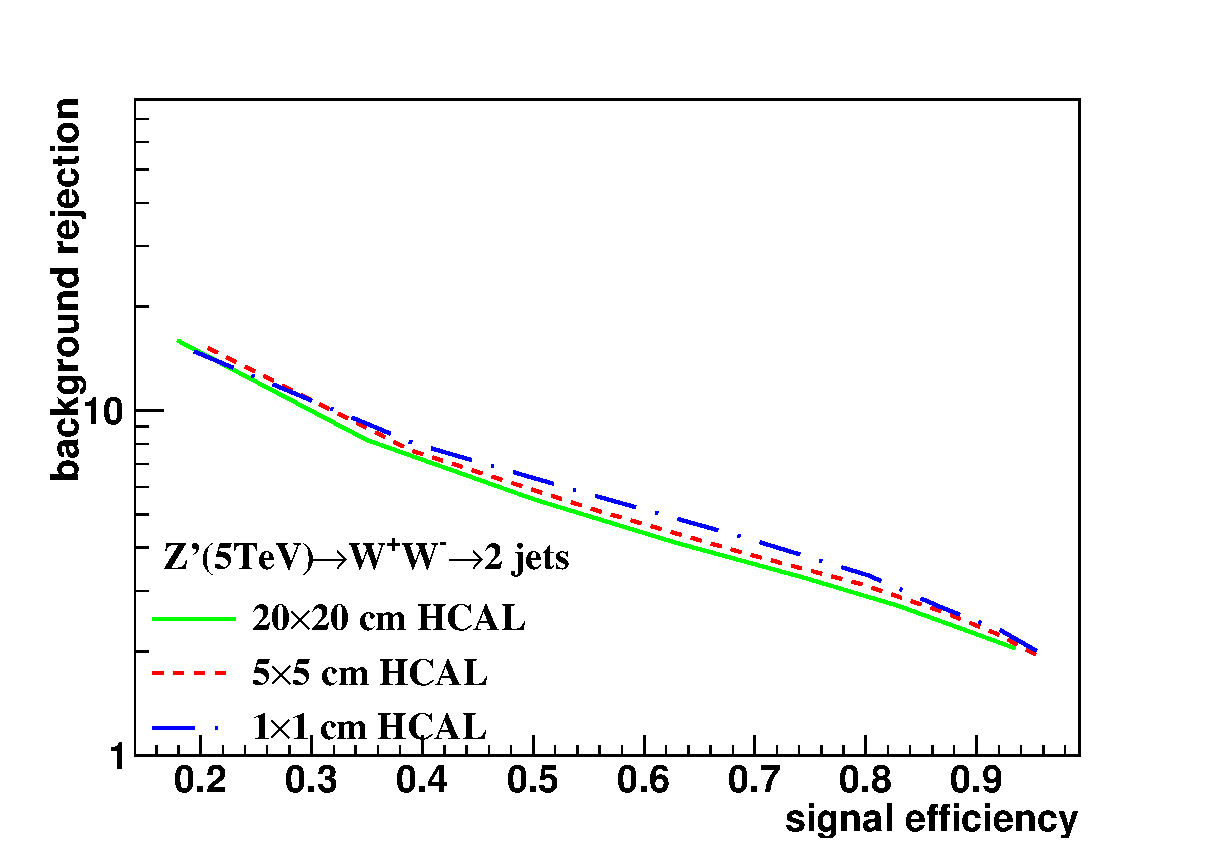
\includegraphics[width=0.43\textwidth]{figs/A_Cluster_mass_sdb2_5tev_eff_1_central_fix_ww_qq_log.eps}
  }
  \subfigure[Central at Median($20\times20$=155,$5\times5$=140,$1\times1$=145) change width in cluster at 10TeV] {
  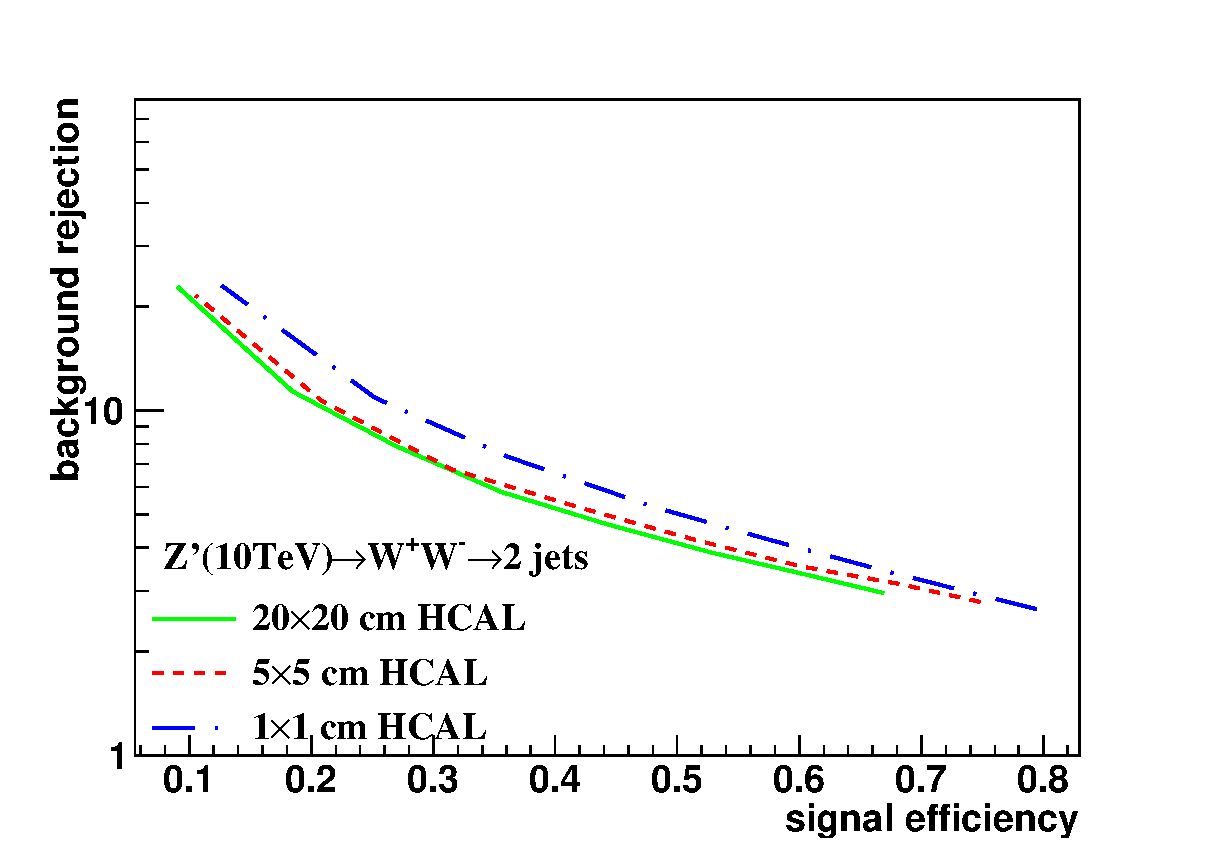
\includegraphics[width=0.43\textwidth]{figs/A_Cluster_mass_sdb2_10tev_eff_1_central_fix_ww_qq_log.eps}
  }
 \subfigure[Central at Median($20\times20$=250,$5\times5$=195,$1\times1$=205) change width in cluster at 20TeV] {
 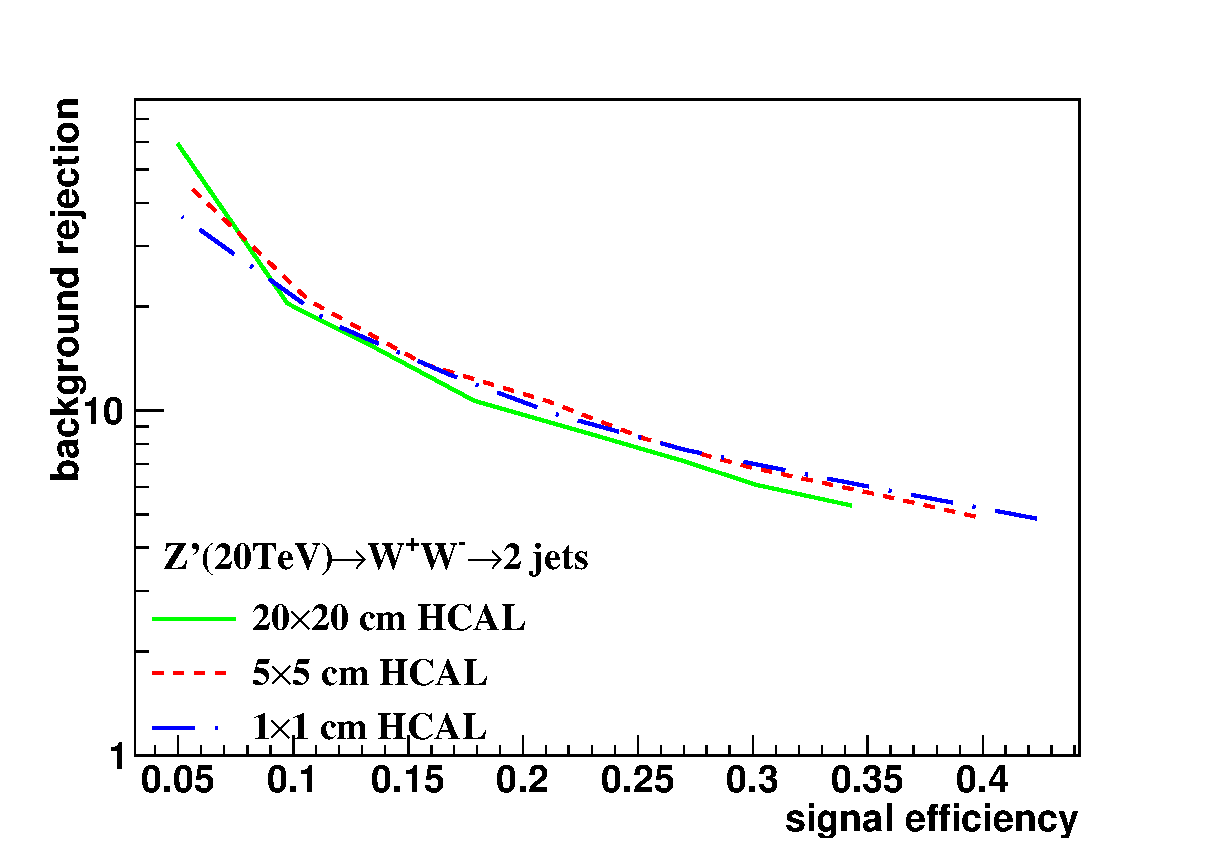
\includegraphics[width=0.43\textwidth]{figs/A_Cluster_mass_sdb2_20tev_eff_1_central_fix_ww_qq_log.eps}
 }
 \subfigure[Central at Median($20\times20$=285,$5\times5$=310,$1\times1$=290) change width in cluster at 40TeV] {
 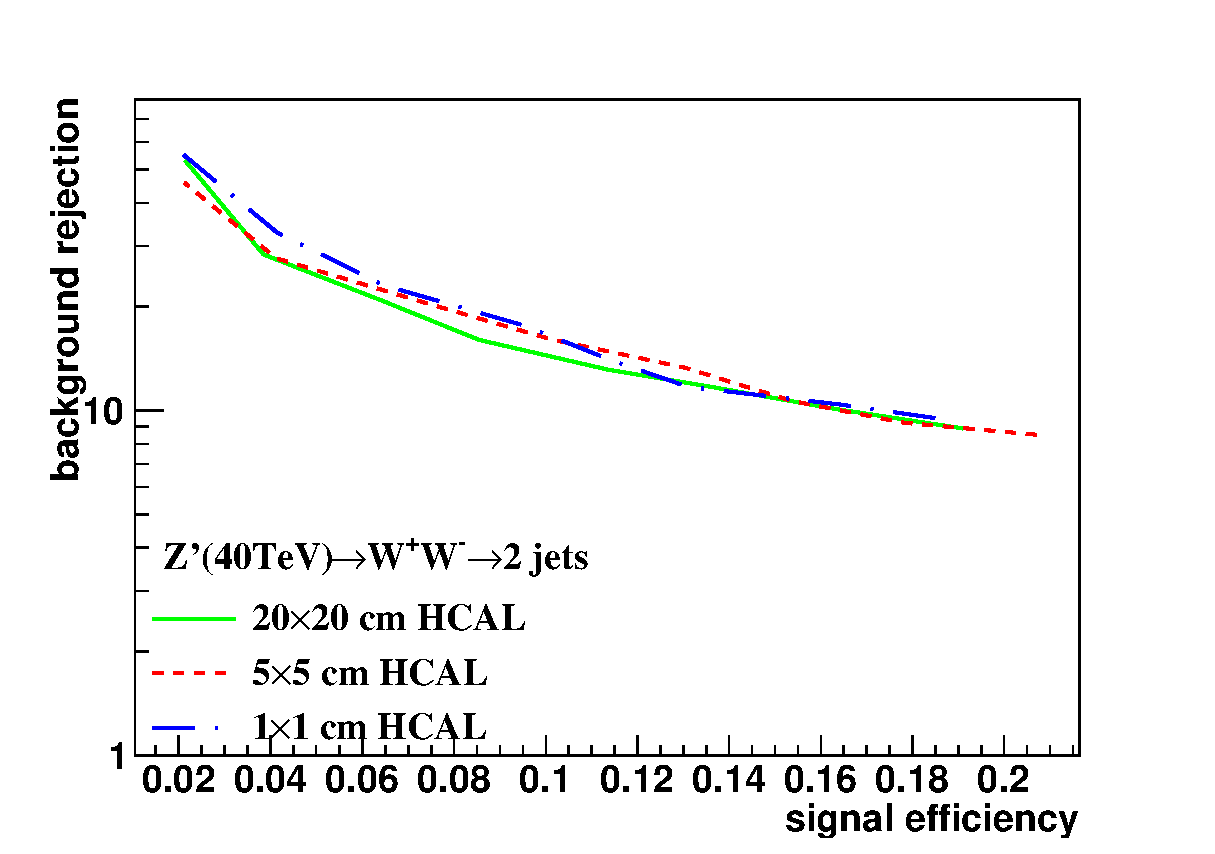
\includegraphics[width=0.43\textwidth]{figs/A_Cluster_mass_sdb2_40tev_eff_1_central_fix_ww_qq_log.eps}
 }
\end{center}
\caption{study of "fix central and change width" in mass soft drop at $\beta$=2, signal=ww, in 5, 10, 20, 40TeV energy of collision  in different detector sizes. Cell Size in 20$\times$20, 5$\times$5, and 1$\times$1(cm$\times$cm) are shown in each picture.}
\label{fig:cluster_tau21_tau32}
\end{figure}

\begin{figure}
\begin{center}
   \subfigure[5TeV at 20$\times$20(cm$\times$cm) in cluster] {
   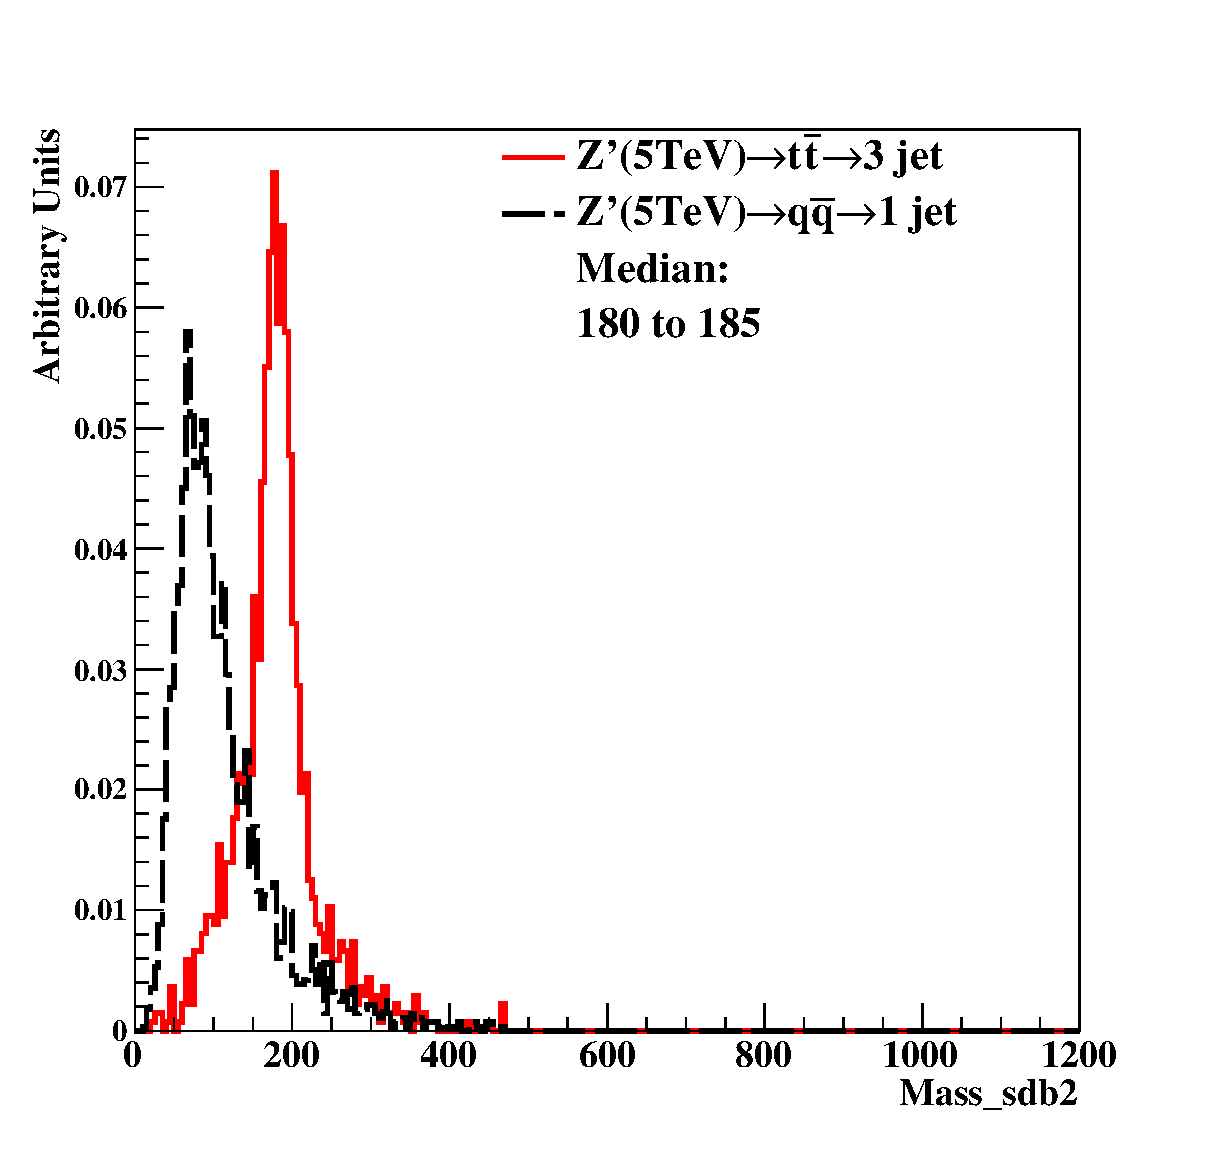
\includegraphics[width=0.22\textwidth]{figs/Dis_cluster_012_mass_sdb2_tt_5tev_04_tt_1200.eps}
   }
      \subfigure[10TeV at 20$\times$20(cm$\times$cm) in cluster] {
   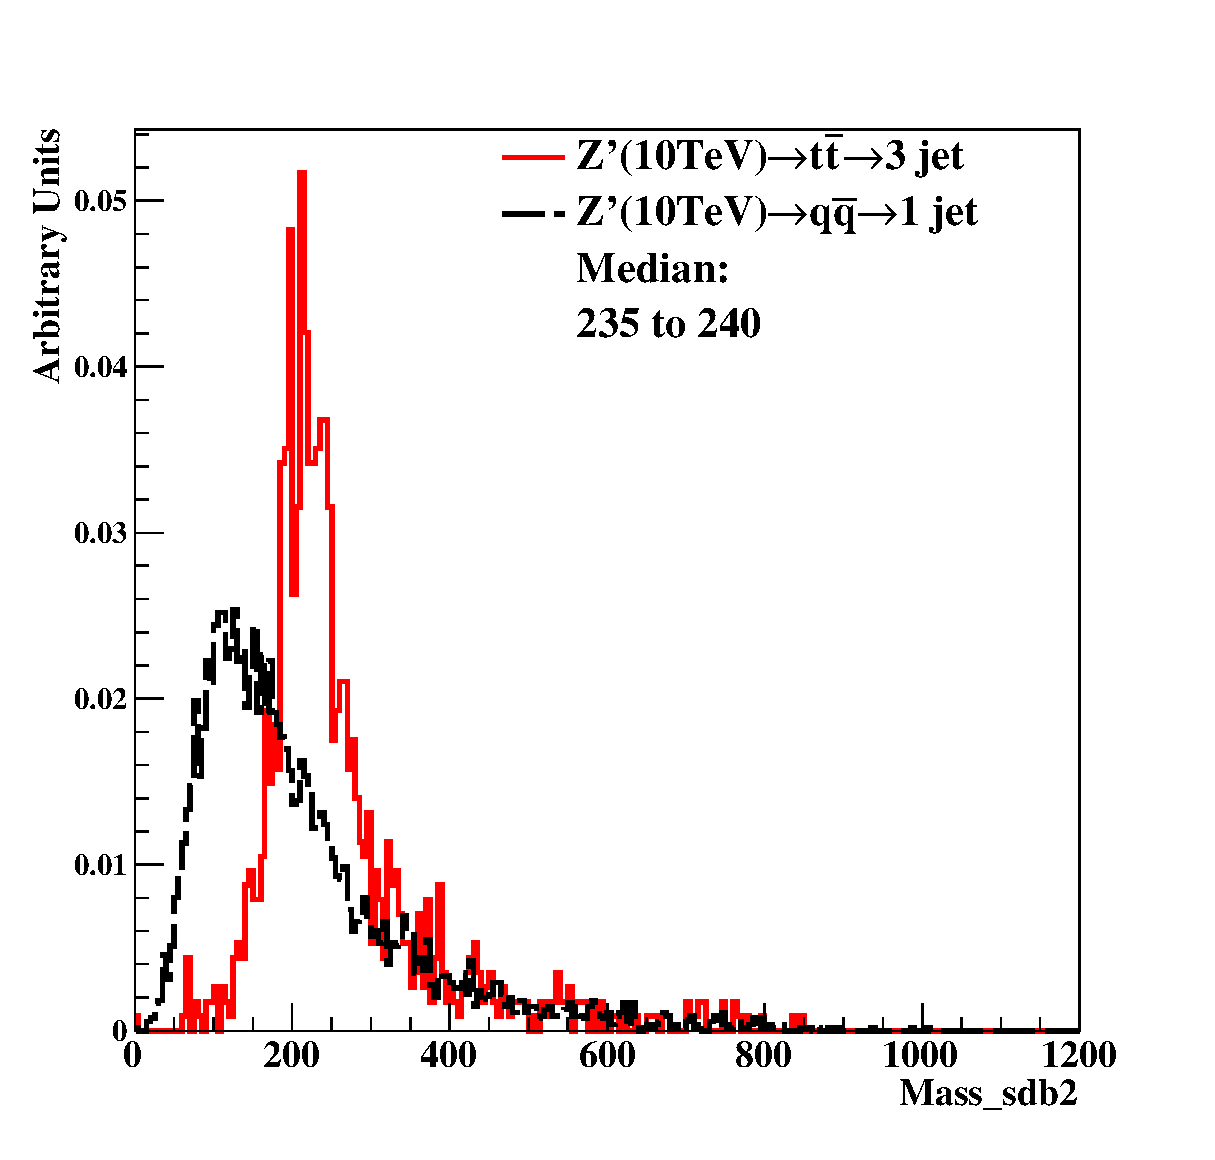
\includegraphics[width=0.22\textwidth]{figs/Dis_cluster_010_mass_sdb2_tt_10tev_04_tt_1200.eps}
   }
   \subfigure[20TeV at 20$\times$20(cm$\times$cm) in cluster] {
   \includegraphics[width=0.22\textwidth]{figs/Dis_cluster_010_mass_sdb2_tt_20tev_04_tt_2400.eps}
   }
    \subfigure[40TeV at 20$\times$20(cm$\times$cm) in cluster] {
   \includegraphics[width=0.22\textwidth]{figs/Dis_cluster_010_mass_sdb2_tt_40tev_04_tt_2400.eps}
   }
   \subfigure[5TeV at 5$\times$5(cm$\times$cm) in cluster] {
   \includegraphics[width=0.22\textwidth]{figs/Dis_cluster_009_mass_sdb2_tt_5tev_04_tt_1200.eps}
   }
   \subfigure[10TeV at 5$\times$5(cm$\times$cm) in cluster] {
   \includegraphics[width=0.22\textwidth]{figs/Dis_cluster_009_mass_sdb2_tt_10tev_04_tt_1200.eps}
   }
   \subfigure[20TeV at 5$\times$5(cm$\times$cm) in cluster] {
   \includegraphics[width=0.22\textwidth]{figs/Dis_cluster_009_mass_sdb2_tt_20tev_04_tt_2400.eps}\hfill
   }
      \subfigure[40TeV at 5$\times$5(cm$\times$cm) in cluster] {
   \includegraphics[width=0.22\textwidth]{figs/Dis_cluster_009_mass_sdb2_tt_40tev_04_tt_2400.eps}\hfill
   }
   \subfigure[5TeV at 1$\times$1(cm$\times$cm) in cluster] {
   \includegraphics[width=0.22\textwidth]{figs/Dis_cluster_012_mass_sdb2_tt_5tev_04_tt_1200.eps}\hfill
   }
    \subfigure[10TeV at 1$\times$1(cm$\times$cm) in cluster] {
   \includegraphics[width=0.22\textwidth]{figs/Dis_cluster_012_mass_sdb2_tt_10tev_04_tt_1200.eps}
   }
   \subfigure[20TeV at 1$\times$1(cm$\times$cm) in cluster] {
   \includegraphics[width=0.22\textwidth]{figs/Dis_cluster_012_mass_sdb2_tt_20tev_04_tt_2400.eps}\hfill
   }
      \subfigure[40TeV at 1$\times$1(cm$\times$cm) in cluster] {
   \includegraphics[width=0.22\textwidth]{figs/Dis_cluster_012_mass_sdb2_tt_40tev_04_tt_2400.eps}
   }
\end{center}
\caption{Distributions of mass soft drop at $\beta$=2, signal=tt, in 5,10TeV energy of collision  in different detector sizes. Cell Size in 20$\times$20, 5$\times$5, and 1$\times$1(cm$\times$cm) are shown here.}
\label{fig:cluster_tau21_tau32}
\end{figure}


\begin{figure}
\begin{center}
  \subfigure[Central at Median($20\times20$=185,$5\times5$=185,$1\times1$=185) change width in cluster at 5TeV] {
  \includegraphics[width=0.43\textwidth]{figs/A_Cluster_mass_sdb2_5tev_eff_1_central_fix_tt_qq_log.eps}
  }
  \subfigure[Central at Median($20\times20$=240,$5\times5$=240,$1\times1$=240) change width in cluster at 10TeV] {
  \includegraphics[width=0.43\textwidth]{figs/A_Cluster_mass_sdb2_10tev_eff_1_central_fix_tt_qq_log.eps}
  }
 \subfigure[Central at Median($20\times20$=360,$5\times5$=375,$1\times1$=365) change width in cluster at 20TeV] {
 \includegraphics[width=0.43\textwidth]{figs/A_Cluster_mass_sdb2_20tev_eff_1_central_fix_tt_qq_log.eps}
 }
 \subfigure[Central at Median($20\times20$=620,$5\times5$=625,$1\times1$=630) change width in cluster at 40TeV] {
 \includegraphics[width=0.43\textwidth]{figs/A_Cluster_mass_sdb2_40tev_eff_1_central_fix_tt_qq_log.eps}
 }
\end{center}
\caption{study of "fix central and change width" in mass soft drop at $\beta$=2, signal=tt, in 5, 10, 20, 40TeV energy of collision  in different detector sizes. Cell Size in 20$\times$20, 5$\times$5, and 1$\times$1(cm$\times$cm) are shown in each picture.}
\label{fig:cluster_tau21_tau32}
\end{figure}





